\documentclass[]{article}
\usepackage{lmodern}
\usepackage{amssymb,amsmath}
\usepackage{ifxetex,ifluatex}
\usepackage{fixltx2e} % provides \textsubscript
\ifnum 0\ifxetex 1\fi\ifluatex 1\fi=0 % if pdftex
  \usepackage[T1]{fontenc}
  \usepackage[utf8]{inputenc}
\else % if luatex or xelatex
  \ifxetex
    \usepackage{mathspec}
  \else
    \usepackage{fontspec}
  \fi
  \defaultfontfeatures{Ligatures=TeX,Scale=MatchLowercase}
\fi
% use upquote if available, for straight quotes in verbatim environments
\IfFileExists{upquote.sty}{\usepackage{upquote}}{}
% use microtype if available
\IfFileExists{microtype.sty}{%
\usepackage{microtype}
\UseMicrotypeSet[protrusion]{basicmath} % disable protrusion for tt fonts
}{}
\usepackage[margin=1in]{geometry}
\usepackage{hyperref}
\hypersetup{unicode=true,
            pdftitle={PROYECTO PIRHI},
            pdfborder={0 0 0},
            breaklinks=true}
\urlstyle{same}  % don't use monospace font for urls
\usepackage{graphicx,grffile}
\makeatletter
\def\maxwidth{\ifdim\Gin@nat@width>\linewidth\linewidth\else\Gin@nat@width\fi}
\def\maxheight{\ifdim\Gin@nat@height>\textheight\textheight\else\Gin@nat@height\fi}
\makeatother
% Scale images if necessary, so that they will not overflow the page
% margins by default, and it is still possible to overwrite the defaults
% using explicit options in \includegraphics[width, height, ...]{}
\setkeys{Gin}{width=\maxwidth,height=\maxheight,keepaspectratio}
\IfFileExists{parskip.sty}{%
\usepackage{parskip}
}{% else
\setlength{\parindent}{0pt}
\setlength{\parskip}{6pt plus 2pt minus 1pt}
}
\setlength{\emergencystretch}{3em}  % prevent overfull lines
\providecommand{\tightlist}{%
  \setlength{\itemsep}{0pt}\setlength{\parskip}{0pt}}
\setcounter{secnumdepth}{5}

%%% Use protect on footnotes to avoid problems with footnotes in titles
\let\rmarkdownfootnote\footnote%
\def\footnote{\protect\rmarkdownfootnote}

%%% Change title format to be more compact
\usepackage{titling}

% Create subtitle command for use in maketitle
\newcommand{\subtitle}[1]{
  \posttitle{
    \begin{center}\large#1\end{center}
    }
}

\setlength{\droptitle}{-2em}
  \title{Protocolo técnico-social de priorización de la inversión en mejoramiento de la eficiencia de conducción hídrica.}
  \pretitle{\vspace{\droptitle}\centering\huge}
  \posttitle{\par}
  \author{}
  \preauthor{}\postauthor{}
  \date{}
  \predate{}\postdate{}

\usepackage{geometry}
\geometry{letterpaper}
\usepackage{graphicx}
\usepackage{amssymb}
\usepackage{hyperref}
\usepackage{titlesec}
\usepackage{appendix}  
\usepackage{booktabs}
\usepackage{longtable}
\usepackage{multirow}
\usepackage{subcaption}
\usepackage{rotating}

\usepackage{fontspec,xltxtra,xunicode}
\defaultfontfeatures{Mapping=tex-text}
\setmainfont[		
 BoldFont={Century Gothic Bold}, 
 ItalicFont={Century Gothic Italic},
 BoldItalicFont={Century Gothic Bold Italic}
 ]{Century Gothic}
 
 \usepackage[labelfont=bf,font=small,justification=justified]{caption}[2008/04/01] %numeracion con punto y no dos puntos
\DeclareCaptionLabelSeparator{punto}{. } %numeracion con punto
\captionsetup{labelsep=punto} %numeracion con punto
 

\renewcommand{\figurename}{Figura}
\renewcommand{\tablename}{Cuadro} 
\renewcommand{\contentsname}{Tabla de contenidos\\} 
\renewcommand{\listfigurename}{Índice de figuras\\}
\renewcommand{\listtablename}{Índice de cuadros\\} 
\renewcommand{\appendixname}{Anexos}
\renewcommand{\appendixtocname}{Anexos}
\renewcommand{\appendixpagename}{Anexos}
\renewcommand{\thefootnote}{\fnsymbol{footnote}} % numeración por símbolos

\titleformat*{\section}{\normalsize\bfseries}
\titleformat*{\subsection}{\normalsize\bfseries}
\titleformat*{\subsubsection}{\normalsize\bfseries}

\usepackage{fancyvrb}
\newcommand{\VerbBar}{|}
\newcommand{\VERB}{\Verb[commandchars=\\\{\}]}
\DefineVerbatimEnvironment{Highlighting}{Verbatim}{commandchars=\\\{\}}
% Add ',fontsize=\small' for more characters per line
\usepackage{color}
\usepackage{framed}
\usepackage{tabulary}
\definecolor{shadecolor}{RGB}{248,248,248}
\newenvironment{Shaded}{\begin{snugshade}}{\end{snugshade}}
\newcommand{\KeywordTok}[1]{\textcolor[rgb]{0.13,0.29,0.53}{\textbf{#1}}}
\newcommand{\DataTypeTok}[1]{\textcolor[rgb]{0.13,0.29,0.53}{#1}}
\newcommand{\DecValTok}[1]{\textcolor[rgb]{0.00,0.00,0.81}{#1}}
\newcommand{\BaseNTok}[1]{\textcolor[rgb]{0.00,0.00,0.81}{#1}}
\newcommand{\FloatTok}[1]{\textcolor[rgb]{0.00,0.00,0.81}{#1}}
\newcommand{\ConstantTok}[1]{\textcolor[rgb]{0.00,0.00,0.00}{#1}}
\newcommand{\CharTok}[1]{\textcolor[rgb]{0.31,0.60,0.02}{#1}}
\newcommand{\SpecialCharTok}[1]{\textcolor[rgb]{0.00,0.00,0.00}{#1}}
\newcommand{\StringTok}[1]{\textcolor[rgb]{0.31,0.60,0.02}{#1}}
\newcommand{\VerbatimStringTok}[1]{\textcolor[rgb]{0.31,0.60,0.02}{#1}}
\newcommand{\SpecialStringTok}[1]{\textcolor[rgb]{0.31,0.60,0.02}{#1}}
\newcommand{\ImportTok}[1]{#1}
\newcommand{\CommentTok}[1]{\textcolor[rgb]{0.56,0.35,0.01}{\textit{#1}}}
\newcommand{\DocumentationTok}[1]{\textcolor[rgb]{0.56,0.35,0.01}{\textbf{\textit{#1}}}}
\newcommand{\AnnotationTok}[1]{\textcolor[rgb]{0.56,0.35,0.01}{\textbf{\textit{#1}}}}
\newcommand{\CommentVarTok}[1]{\textcolor[rgb]{0.56,0.35,0.01}{\textbf{\textit{#1}}}}
\newcommand{\OtherTok}[1]{\textcolor[rgb]{0.56,0.35,0.01}{#1}}
\newcommand{\FunctionTok}[1]{\textcolor[rgb]{0.00,0.00,0.00}{#1}}
\newcommand{\VariableTok}[1]{\textcolor[rgb]{0.00,0.00,0.00}{#1}}
\newcommand{\ControlFlowTok}[1]{\textcolor[rgb]{0.13,0.29,0.53}{\textbf{#1}}}
\newcommand{\OperatorTok}[1]{\textcolor[rgb]{0.81,0.36,0.00}{\textbf{#1}}}
\newcommand{\BuiltInTok}[1]{#1}
\newcommand{\ExtensionTok}[1]{#1}
\newcommand{\PreprocessorTok}[1]{\textcolor[rgb]{0.56,0.35,0.01}{\textit{#1}}}
\newcommand{\AttributeTok}[1]{\textcolor[rgb]{0.77,0.63,0.00}{#1}}
\newcommand{\RegionMarkerTok}[1]{#1}
\newcommand{\InformationTok}[1]{\textcolor[rgb]{0.56,0.35,0.01}{\textbf{\textit{#1}}}}
\newcommand{\WarningTok}[1]{\textcolor[rgb]{0.56,0.35,0.01}{\textbf{\textit{#1}}}}
\newcommand{\AlertTok}[1]{\textcolor[rgb]{0.94,0.16,0.16}{#1}}
\newcommand{\ErrorTok}[1]{\textcolor[rgb]{0.64,0.00,0.00}{\textbf{#1}}}
\newcommand{\NormalTok}[1]{#1}
\usepackage{graphicx,grffile}
\makeatletter
\def\maxwidth{\ifdim\Gin@nat@width>\linewidth\linewidth\else\Gin@nat@width\fi}
\def\maxheight{\ifdim\Gin@nat@height>\textheight\textheight\else\Gin@nat@height\fi}
\makeatother
\usepackage{booktabs}
\usepackage{longtable}
\usepackage{array}
\usepackage{multirow}
\usepackage[table]{xcolor}
\usepackage{wrapfig}
\usepackage{float}
\usepackage{colortbl}
\usepackage{pdflscape}
\usepackage{tabu}
\usepackage{threeparttable}
\usepackage[normalem]{ulem}
\usepackage[none]{hyphenat}
\usepackage{multicol}
\usepackage{tabularx}
\usepackage{rotating}
\usepackage{colortbl}
\usepackage{lscape}
\usepackage{footnote}

% Regla con color
\makeatletter
\let\old@rule\@rule
\def\@rule[#1]#2#3{\textcolor{rulecolor}{\old@rule[#1]{#2}{#3}}}
\makeatother
% Cambiar color de regla
\definecolor{rulecolor}{RGB}{183,183,183}

% Color para las letras del título
\definecolor{casinegro}{RGB}{71,71,71}

\begin{document}
\sloppy 

\newgeometry{left=3cm,bottom=0cm,top=1cm,right=3cm}

\begin{titlepage}

\begin{figure} [H]
  
\includegraphics[width=.2\textwidth]{Logo/bg_gob_logo.png}
\end{figure}

\fontsize{15}{0} \selectfont{\textbf{\textcolor{casinegro}{``PLANIFICACIÓN DE LA INVERSIÓN EN REVESTIMIENTOS HÍDRICOS"}}} \vspace*{.1in}\\ % el inicio de comillas simples es ` y de doble es de ``.
\fontsize{15}{0} \selectfont{\textcolor{casinegro}{FIC-R 2016}}\\
\rule{10cm}{.05cm}
\vspace*{.1in}
\hspace*{.2in}

\fontsize{14}{0} \selectfont{\textcolor{casinegro}{Universidad de La Serena}} \vspace*{.1in}\\
\fontsize{14}{0} \selectfont{\textbf{\textcolor{casinegro}{Región de Coquimbo}}}

\vspace*{.1in}

\begin{figure}[H]
  \centering
\begin{subfigure}[c]{.2\textwidth}
  
\includegraphics[width=\textwidth]{Logo/GOB_RGB.png}
\end{subfigure}
\hfill
\begin{subfigure}[c]{.23\textwidth}
  
\includegraphics[width=\textwidth]{Logo/uls.png} 
\end{subfigure}
\end{figure}
\vspace*{4in}

\begin{figure}[H]
  \centering
\begin{subfigure}{.74\textwidth}
   \fontsize{14}{0} \selectfont{\textcolor{casinegro}{Mayo 2018}} \\
   {\definecolor{rulecolor}{named}{casinegro}\rule[-3mm]{10cm}{.05cm}}
\end{subfigure}
\hfill
\begin{subfigure}{.25\textwidth}
\hfill
  
\includegraphics[width=\textwidth]{Logo/lgore.pdf} 
\end{subfigure}
\end{figure}


\end{titlepage}

\restoregeometry


\begin{table}[!htb]
\centering \vspace*{2.5in}
\arrayrulecolor{cyan}
\begin{tabular}{|l|l|l|l|}
    \hline 
    \multicolumn{3}{|c|}{\multirow{2}{8cm}{\centering \textbf{INFORME DE AVANCE TÉCNICO} \\
    \textbf{FIC REGIONAL} }} & \textbf{Fecha de emisión:}\\
    \cline{4-4}
    \multicolumn{3}{|c|}{\multirow{2}{8cm}} &  Mayo 2018\\
    \hline
    \textbf{Fecha de inicio:}  &\textbf{Fecha de término:} &\textbf{N° de informe:} &\textbf{Duración:}\\
     20/Diciembre/2017 & 20/Octubre/2019 & 1 & 22 meses\\
    \hline
    \textbf{Nombre del proyecto:} & \multicolumn{3}{|l|}{\textbf{Planificación de la Inversión en Revestimientos Hídricos}}\\
    \hline
    \multirow{4}{4cm}{\textbf{Financiamiento:}} & \textbf{Monto total del proyecto:} & \multicolumn{2}{c|}{\centering M\$ 222.188}\\
    \cline{2-4}
    & \multirow{2}{4cm}{\textbf{Aporte FIC-R:}} & \multicolumn{2}{c|}{\textbf{Año 1:} M\$ 90.040}\\
    \cline{3-4}
    & & \multicolumn{2}{c|}{\textbf{Año 2:} M\$ 109.928}\\
    \cline{2-4}
    & \textbf{Aporte institución:} & \multicolumn{2}{c|}{\centering M\$ 22.220}\\
    \hline
    \textbf{Institución ejecutora:} & \multicolumn{3}{|l|}{\centering Universidad de La Serena}\\
    \hline
    \textbf{Responsable del proyecto:} & \multicolumn{3}{|l|}{\centering Dr. Pablo Álvarez Latorre}\\
    \hline
    \textbf{Cargo:} & \multicolumn{3}{|l|}{\centering Director del proyecto}\\
    \hline
    \textbf{E-mail:} & \multicolumn{3}{|l|}{\centering pabloa@userena.cl}\\
    \hline
    \textbf{Fono:} & \multicolumn{3}{|l|}{\centering 51-2554913}\\
    \hline

\end{tabular}

\end{table}

\clearpage

\tableofcontents

\clearpage

\section{Resumen del Proyecto}

La iniciativa denominada ``Planificación de la Inversión en Revestimientos Hídricos", se adjudicó un financiamiento FIC de \$ 199.968.000, lo que sumado a los aportes de la contraparte totalizan \$ 220.188.000. Ejecutándose desde Diciembre de 2017 a Octubre de 2019, por un período de 22 meses.\\
\\
El proyecto tiene por finalidad planificar el mejoramiento de la eficiencia de conducción hídrica, a través de la transferencia de conocimientos y herramientas a las Organizaciones de Usuarios de Aguas (OUA's) para apoyar la gestión de recursos hídricos. El impacto directo o propósito es incrementar la oferta neta, por medio de la priorización de las inversiones público-privadas basados en parámetros técnico-social.\\
\\
El área en la cual se desarrolla esta iniciativa corresponde a la cuenca del río Choapa, abarcando toda el área de influencia de la Junta de Vigilancia del río Chalinga y sus Afluentes, la Junta de Vigilancia del río Illapel y sus Afluentes, y la Junta de Vigilancia del río Choapa y sus Afluentes. Por lo mismo, las instituciones asociadas al proyecto son la Junta de Vigilancia del río Chalinga y sus Afluentes, la Junta de Vigilancia del río Illapel y sus afluentes, y la Junta de Vigilancia del río Choapa y sus Afluentes, además como beneficiarios indirectos la Fundación Minera Los Pelambres e instituciones públicas como la Dirección de Obras Hidráulicas y la Comisión Nacional de Riego.\\
\\
Los resultados esperados de este proyecto son:
\begin{itemize}
\item Protocolo técnico-social de priorización de la inversión en mejoramiento de la eficiencia de conducción hídrica.
\item Plan de priorización de la inversión en mejoramiento de la eficiencia de conducción hídrica para la red de distribución de la Junta de Vigilancia Río Chalinga y sus Afluentes.
\item Plan de priorización de la inversión en mejoramiento de la eficiencia de conducción hídrica para la red de distribución de la Junta de Vigilancia Río Illapel y sus Afluentes.
\item Plan de priorización de la inversión en mejoramiento de la eficiencia de conducción hídrica para la red de distribución en la Junta de Vigilancia Río Choapa y sus Afluentes.
\item Programa de capacitación en gestión hídrica.
\item Sistema virtual de priorización de la inversión en mejoramiento de la eficiencia de conducción hídrica para las cuencas del río Choapa.
\item Protocolo técnico-social de priorización de la inversión en mejoramiento de la eficiencia de conducción hídrica.
\end{itemize}

El mérito innovador del proyecto se visualiza en establecer bases para la gestión integrada de los recursos hídricos de la cuenca, a través de un ordenamiento de la inversión en mejoramiento de eficiencia de conducción, por medio de la modelación dinámica del sistema hídrico.\\
\\
El equipo de trabajo de este proyecto está constituido por profesionales del Laboratorio de Prospección, Monitoreo y Modelación de Recursos Agrícolas y Ambientales (PROMMRA) perteneciente al Departamento de Agronomía de la Universidad de La Serena, liderado por el Dr. Pablo Álvarez Latorre.\\
\clearpage

\section{Resumen del período a informar}

El proyecto FIC-R 2016 - Planificación de la Inversión en Revestimientos Hídricos - código BIP 30485958-0, comenzó con su ejecución el 20 de Diciembre de 2017. En este informe se presenta el avance de ejecución de la componente 1, que abarca el período entre el 20 de Diciembre de 2017 y el 20 de Mayo de 2018.\\
\\
Según carta Gantt del proyecto, se ejecutaron las siguientes actividades:
\begin{itemize}
\item Diagnóstico técnico-social del Protocolo de Priorización de Inversiones en Mejoramiento de la Eficiencia de Conducción Hídrica: Se realizó una revisión y diagnóstico del protocolo diseñado en el proyecto SIMCA - ELQUI, en función de los componentes técnicos y sociales, generando una propuesta de fortalecimiento.
\item Definición parámetros y generación del protocolo de las variables superficie bajo riego y potencial: Se definió los parámetros a incorporar en esta variable, además de generar el protocolo que permite incorporar estos criterios técnicos de superficie bajo riego ($ha$) y potencial ($ha$) asociada al área de influencia de cada canal, al protocolo 
\item Definición de parámetros y generación de los protocolos para la variable modelamiento hidrológico: Se definió los parámetros que permitan incorporar la variable modelamiento hidrológico, además de generar el protocolo que permita considerar los efectos dinámicos del mejoramiento en la eficiencia de conducción en las cuencas.
\item Validación del Protocolo técnico-social de inversión en mejoramiento de la eficiencia de conducción hídrica.
\end{itemize}

%Además se ha comenzado con el desarrollo de las actividades de la componente 2. Plan de priorización de la inversión en mejoramiento de la eficiencia de conducción hídrica para la red de distribución de la Junta de Vigilancia del río Chalinga y sus afluentes.

%\begin{itemize}
%\item SIG Red de distribución y conducción hídrica de Junta de Vigilancia Río Chalinga y sus afluentes.
%\item Determinación de pérdidas canales Junta de Vigilancia Río Chalinga y sus Afluentes.
%\item Evaluación superficie bajo riego y superficie potencial de las zonas de riego de la Junta de Vigilancia Río Chalinga y sus Afluentes.
%\item Transferencia de capacidades en la aplicación del protocolo técnico-social de la inversión en mejoramiento de la eficiencia de conducción hídrica.
%\end{itemize}

\clearpage
\section{Actividades programadas y ejecutadas}
\begin{table}[!htb]
\centering
\resizebox{16cm}{!} {
\begin{tabular}{|p{3cm}|p{1.6cm}|p{3.9cm}|p{2.5cm}|p{2.5cm}|p{1.5cm}|}
    \hline
    \textbf{Componente} & \textbf{N° Actividad} & \textbf{Actividades Programadas} & \textbf{Actividades Ejecutadas} & \textbf{Discrepancias} & \textbf{\% de avance físico}\\
    \hline
    \multirow {4}{3cm}{1. Protocolo técnico-social de Priorización de la Inversión en Mejoramiento de la Eficiencia de Conducción Hídrica} & 1 & 		Diagnóstico técnico-social del Protocolo de Priorización de Inversiones en Mejoramiento de la eficiencia de Conducción Hídrica &  Ejecutada (E)  & No & 100\%\\
    \cline{2-6}
    & 2 & Definición parámetros y generación del protocolo de las variables superficie bajo riego y potencial & Ejecutada (E) & No & 100\%\\
    \cline{2-6}
    & 3 & Definición de parámetros y generación del protocolo para la variable modelamiento hidrológico & Ejecutada (E)  & No & 100\%\\
    \cline{2-6}
    & 4 & Validación del protocolo técnico-social de inversión en mejoramiento de la eficiencia en conducción hídrica & Ejecutada (E)  & No & 100\%\\
    \hline
%    \multirow {4}{3cm}{2. Plan de priorización de la inversión en mejoramiento de la eficiencia de conducción hídrica para la red de distribución de la Junta de Vigilancia del río Chalinga y sus afluentes} & 		1 & 		SIG Red de distribución y conducción hídrica de Junta de Vigilancia Río Chalinga y sus afluentes & En Ejecución (EE)      		& No & 30\%\\ \cline{2-6}
%    & 2 & Determinación de pérdidas canales Junta de Vigilancia Río Chalinga y sus Afluentes & En Ejecución (EE)      		& No & 15\%\\ \cline{2-6}
%    & 3 & Evaluación superficie bajo riego y superficie potencial de las zonas de riego de la Junta de Vigilancia Chalinga y sus Afluentes & En Ejecución (EE)      		& No & 15\%\\ \cline{2-6}
%    & 5 & Transferencia de capacidades en la aplicación del protocolo técnico-social de la inversión en mejoramiento de la eficiencia de conducción hídrica & En Ejecución (EE)      		& No & 15\%\\
%    \hline
   
\end{tabular}
}
\end{table}

\clearpage


\section{Razones que explican las discrepancias entre actividades programadas y las efectivamente realizadas}



\clearpage
\section{Carta Gantt}

\begin{table}[!htb]
\centering
\arrayrulecolor{black}
\resizebox{17cm}{!} {
\begin{tabular}{|l|c|c|c|c|c|c|c|c|c|c|c|c|c|c|c|c|c|c|c|c|c|c|c|}
    \hline
    \multirow{2}{2cm}{\textbf{RESULTADOS}} & \multicolumn{12}{|c|}{\textbf{Año 1}} & \multicolumn{10}{|c|}{\textbf{Año 2}}\\
    \cline{2-23}
    & m1 & m2 & m3 & m4 & m5 & m6 & m7 & m8 & m9 & m10 & m11 & m12 & m13 & m14 & m15 & m16 & m17 & m18 & m19 & m20 & m21 & m22\\ \hline
    \textbf{Componente 1} & \multicolumn{22}{|l|}{}\\ \hline
    Actividad 1.1 & \cellcolor{yellow}X & \cellcolor{yellow}X & \cellcolor{yellow}X &\cellcolor{yellow}X & & & & & & & & & & & & & & & & & & \\ \hline
    Actividad 1.2 & & & \cellcolor{yellow}X & \cellcolor{yellow}X & \cellcolor{yellow}X & & & & & & & & & & & & & & & & & \\ \hline
    Actividad 1.3 & & & \cellcolor{yellow}X & \cellcolor{yellow}X & \cellcolor{yellow}X & & & & & & & & & & & & & & & & & \\ \hline
    Actividad 1.4 & & & & \cellcolor{yellow}X & \cellcolor{yellow}X & & & & & & & & & & & & & & & & & \\ \hline
    \textbf{Componente 2} & \multicolumn{22}{|l|}{}\\ \hline
    Actividad 2.1 & & & & X & X & X & X & X & X & X & & & & & & & & & & & & \\ \hline
    Actividad 2.2 & & & & & X & X & X & X & X & X & & & & & & & & & & & & \\ \hline
    Actividad 2.3 & & & & & & & & X & X & X & & & & & & & & & & & & \\ \hline
    Actividad 2.4 & & & & & & & & X & X & X & & & & & & & & & & & & \\ \hline
    Actividad 2.5 & & & & X & X & X & X & X & X & X & & & & & & & & & & & & \\ \hline
    Actividad 2.6 & & & & & & & & & X & X & & & & & & & & & & & & \\ \hline
    \textbf{Componente 3} & \multicolumn{22}{|l|}{}\\ \hline
    Actividad 3.1 & & & & & & & & & X & X & X & X & X & X & X & & & & & & & \\ \hline
    Actividad 3.2 & & & & & & & & & & X & X & X & X & X & X & & & & & & & \\ \hline
    Actividad 3.3 & & & & & & & & & & & & & X & X & X & & & & & & & \\ \hline
    Actividad 3.4 & & & & & & & & & & & & & X & X & X & & & & & & & \\ \hline
    Actividad 3.5 & & & & & & & & & X & X & X & X & X & X & X & & & & & & & \\ \hline
    Actividad 3.6 & & & & & & & & & & & & & & X & X & & & & & & & \\ \hline
    \textbf{Componente 4} & \multicolumn{22}{|l|}{}\\ \hline
    Actividad 4.1 & & & & & & & & & & & & & & & X & X & X & X & X & X & X & X\\ \hline
    Actividad 4.2 & & & & & & & & & & & & & & & & X & X & X & X & X & X & X\\ \hline
    Actividad 4.3 & & & & & & & & & & & & & & & & & & & & X & X & X \\ \hline
    Actividad 4.4 & & & & & & & & & & & & & & & & & & & & & X & X\\ \hline
    Actividad 4.5 & & & & & & & & & & & & & & & X & X & X & X & X & X & X & X\\ \hline
    Actividad 4.6 & & & & & & & & & & & & & & & & & & & & & X & X\\ \hline
    \textbf{Componente 5} & \multicolumn{22}{|l|}{}\\ \hline
    Actividad 5.1 & X & & & & & & & & & & & & & & & & & & & & & X\\ \hline
    Actividad 5.2 & & & & & X & & & & & & & & & & & & & & & & & \\ \hline
    Actividad 5.3 & & & & & & & & & & X & & & & & & & & & & & & \\ \hline
    Actividad 5.4 & & & & & & & & & & & & & & X & & & & & & & & \\ \hline
    Actividad 5.5 & & & & & & & & & & & & & & & & & & & X & & & \\ \hline
    \textbf{Componente 6} & \multicolumn{22}{|l|}{}\\ \hline
    Actividad 6.1 & & & & & & & & & & & & & & & X & X & X & X & & & & \\ \hline
    Actividad 6.2 & & & & & & & & & & & & & & & & & X & X & X & X & & \\ \hline
    Actividad 6.3 & & & & & & & & & & & & & & & & & & & & X & X & X\\ \hline
\end{tabular}
}
\end{table}

\clearpage
\section{Cuadro de antecedentes financieros}

\clearpage
\section{Gráfico curva de avance físico v/s programado}

\clearpage
\section{Metodología}

\subsection{Componente 1. Actividad 1.1. Diagnóstico técnico-social del Protocolo de Priorización de Inversiones en Mejoramiento de la eficiencia de Conducción Hídrica}

\begin{table}[!htb]
\centering
\begin{tabular}{|p{2cm}|p{2cm}|p{2cm}|p{2cm}|p{2cm}|p{2cm}|}
    \hline
    \multicolumn{2}{|l|}{Fecha de Inicio} & 20-12-2017 & \multicolumn{2}{l|}{Fecha de Término} & 20-05-2018\\
    \hline
    \multicolumn{6}{|c|}{Presupuesto (M\$)}\\
    \hline
    Total & xxxxx & FIC-R & XXXXXX & ULS & XXXXXX\\
    \hline
    \multicolumn{4}{|l|}{Porcentaje de Avance} & \multicolumn{2}{c|}{100\%}\\
    \hline
\end{tabular}
\end{table}

Se estableció una mesa técnica, compuesta por los profesionales de las diferentes áreas del equipo para la revisión y diagnóstico del protocolo de priorización de inversiones en mejoramiento de la eficiencia de conducción hídrica, generado por el proyecto FIC-R 2013, \textit{``Diseño y puesta en marcha de un sistema de monitoreo de caudales y de un protocolo de determinación de pérdidas de agua, para la priorización de las inversiones público-privadas (SIMCA – ELQUI)"}, el cual tenía por objetivo unificar, estandarizar y normalizar los criterios, procedimientos y decisiones ligadas al mejoramiento de canales pertenecientes a una organización de regantes.\\
\\
La revisión tiene como finalidad identificar las variables requeridas por el protocolo de priorización de inversiones en mejoramiento de la eficiencia de conducción hídrica para su ejecución, junto con la información complementaria para el desarrollo de este, además de su metodología para la captura, tabulación y procesamiento. Además, se realizó un diagnóstico, con el propósito de desarrollar una propuesta de fortalecimiento que permita el uso de los recursos hídricos con un enfoque de cuenca, a través de un manejo integrado y sustentable de los diferentes usuarios de aguas.\\
\\ 
El fortalecimiento de esta herramienta, tiene como objetivo que las OUA's la incorporen en su gestión hídrica, para apoyar la toma de decisiones en la distribución de recursos para inversión en mejoramientos de la eficiencia de conducción hídrica, el cual permitirá obtener un mayor impacto basado en aspectos técnicos y sociales, donde se promueva el crecimiento y desarrollo equitativo, sin interceder en la disponibilidad de los recursos de otras zonas.

\subsection{Componente 1. Actividad 1.2. Definición parámetros y generación de los protocolos de variable superficie bajo riego y superficie potencial.}

\begin{table}[!htb]
\centering
\begin{tabular}{|p{2cm}|p{2cm}|p{2cm}|p{2cm}|p{2cm}|p{2cm}|}
    \hline
    \multicolumn{2}{|l|}{Fecha de Inicio} & 20-12-2017 & \multicolumn{2}{l|}{Fecha de Término} & 20-05-2018\\
    \hline
    \multicolumn{6}{|c|}{Presupuesto (M\$)}\\
    \hline
    Total & xxxxx & FIC-R & XXXXXX & ULS & XXXXXX\\
    \hline
    \multicolumn{4}{|l|}{Porcentaje de Avance} & \multicolumn{2}{c|}{100\%}\\
    \hline
\end{tabular}
\end{table}

La propuesta de fortalecimiento plantea la inclusión de parámetros sociales que permitan el crecimiento y desarrollo equitativo de la zona. Para determinar el área de influencia de la OUA's y Comunidades de aguas, resulta fundamental conocer la superficie asociada a estas. La superficie como parámetro social, establece que los beneficios sobre esta, generan efectos sobre la permanencia de la población en esta, creación de polos productivos y mejoramiento de la calidad de vida a través de la creación de empleos.\\
\\
Los parámetros de superficie se ajustan al área de influencia ligada al recurso hídrico y desarrollo de agricultura, bajo estos supuestos se establecerán los parámetros y se desarrollará el protocolo para la recolección de estos.

\subsection{Componente 1. Actividad 1.3. Definición de parámetros y generación de los protocolos para la variable modelamiento hidrológico.}

\begin{table}[!htb]
\centering
\begin{tabular}{|p{2cm}|p{2cm}|p{2cm}|p{2cm}|p{2cm}|p{2cm}|}
    \hline
    \multicolumn{2}{|l|}{Fecha de Inicio} & 20-12-2017 & \multicolumn{2}{l|}{Fecha de Término} & 20-05-2018\\
    \hline
    \multicolumn{6}{|c|}{Presupuesto (M\$)}\\
    \hline
    Total & xxxxx & FIC-R & XXXXXX & ULS & XXXXXX\\
    \hline
    \multicolumn{4}{|l|}{Porcentaje de Avance} & \multicolumn{2}{c|}{100\%}\\
    \hline
\end{tabular}
\end{table}

Para visualizar los efectos que genera el mejoramiento de la eficiencia de conducción hídrica sobre los componentes hidrológicos de la cuenca, se modelarán estos escenarios a través del modelo WEAP. Esta herramienta ha sido utilizada ampliamente en la planificación y gestión de los recursos hídrico en la región. La consultora RODHOS el 2014, desarrollo tres modelos de gestión para las tres cuencas de la región de Coquimbo, bajo el estudio financiado por el Gobierno Regional denominado “Estudio de modelos de gestión de recursos hídricos superficiales y subterráneos, para las cuencas de las provincias de Elqui, Limarí y Choapa”. Posterior a ello, el Laboratorio PROMMRA de la Universidad de La Serena, actualizó cada uno de estos modelos en su serie temporal, en el marco del estudio (2016) “Análisis Modelación de Embalses de Pre cordillera”, financiado por el Gobierno Regional.\\
\\
Basándose en la última actualización del modelo WEAP para la cuenca del río Choapa, se generará la modelación y evaluación del mejoramiento en las eficiencias de conducción de los canales de la cuenca.\\
\\
La configuración topológica del modelo de gestión de la cuenca del río Choapa, se basa en la agrupación de canales bajo ciertos criterios: superficie regada por canal, distribución de los canales en la cuenca, y ubicación de estos. Esta topología se desarrolló en función de las capacidades técnicas que posee el modelo y la disponibilidad de los datos como \textit{input} asociado a la serie temporal modelada.\\ 
 \\
WEAP, es un modelo semi-distribuido, el cual establece características hidrológicas similares en zonas de la cuenca; de esta manera, la agrupación de canales permite un correcto balance hídrico y calibración de lo sucedido en el sistema, obteniendo resultados zonificados de los efectos hidrológicos del revestimiento en las obras de conducción de la cuenca.\\
\\
La definición de los parámetros de evaluación, se especifican de acuerdo a los resultados que el modelo WEAP es capaz de entregar, asociado a la zonificación de los escenarios y, los efectos hidrológicos que el revestimiento de canales puede generar en otros componentes hidrológicos de la cuenca.\\
\\
Parte del proceso de ajuste del modelo para generar los escenarios de revestimiento, es la confirmación de los datos utilizados en la configuración de los canales y su agrupación. Para ello es necesario disponer de información actualizada de estas obras.\\
\\
Con dicha información, se ajustará el modelo de gestión para las distintas organizaciones y se evaluarán los efectos de revestimiento a partir de la generación de escenarios que el protocolo establece para la variable modelamiento hidrológico.\\
\\
Para dicha variable del protocolo, se establecerán las etapas de actualización de \textit{inputs} en el modelo WEAP, asociado a las comunidades de agua, y la posterior visualización de resultados de los parámetros establecidos, respecto a los escenarios de mejoramiento en la eficiencia de conducción.

\subsection{Componente 1. Actividad 1.4. Validación del protocolo técnico-social de inversión en mejoramiento de la eficiencia en conducción hídrica.}

\begin{table}[!htb]
\centering
\begin{tabular}{|p{2cm}|p{2cm}|p{2cm}|p{2cm}|p{2cm}|p{2cm}|}
    \hline
    \multicolumn{2}{|l|}{Fecha de Inicio} & 20-12-2017 & \multicolumn{2}{l|}{Fecha de Término} & 20-05-2018\\
    \hline
    \multicolumn{6}{|c|}{Presupuesto (M\$)}\\
    \hline
    Total & xxxxx & FIC-R & XXXXXX & ULS & XXXXXX\\
    \hline
    \multicolumn{4}{|l|}{Porcentaje de Avance} & \multicolumn{2}{c|}{100\%}\\
    \hline
\end{tabular}
\end{table}

La incorporación de nuevos parámetros permite el fortalecimiento de esta herramienta para la gestión hídrica de las OUA's, denominado Protocolo técnico-social de inversión en mejoramiento de la eficiencia hídrica.\\
\\
La validación del Protocolo técnico-social de inversión en mejoramiento de la eficiencia de conducción hídrica se aplicará y evaluará en todas sus etapas en tres comunidades de aguas.

\begin{enumerate}
\item Recopilación de información
\begin{itemize}	
	\item Cuenca
	\item OUA's
	\item Comunidad de Aguas
\end{itemize}
\item Sistema de Información Geográfica (S.I.G)
\item Determinación de Pérdidas
\item Superficie bajo riego y potencial
\item Modelación Hidrológica
\item Priorización de canales
\end{enumerate}
\clearpage
\section{Resultados}

\subsection{Componente 1. Actividad 1.1. Diagnóstico del Protocolo de Priorización de Inversiones en Mejoramiento de la eficiencia de Conducción Hídrica}

A través de la revisión realizada al protocolo de priorización de inversiones en mejoramiento de la eficiencia de conducción hídrica, se logró identificar las variables requeridas para generar el plan de priorización de canales y/o tramos de la red de distribución de una OUA's, las cuales se basan en exclusivamente en parámetros técnicos. Además se identificó la información complementaria para el desarrollo de este.\\
\\
El diagnóstico considera la inclusión de nuevos parámetros, basados en aspectos técnicos - sociales, además de la adición de información a nivel de comunidades de aguas para obtener recopilar datos de fuentes primarias, junto con generar el vínculo con los beneficiarios. Para el mejoramiento e incorporación de parámetros, se generó una propuesta de fortalecimiento cuyo objetivo es robustecer los fundamentos de la toma de decisiones en la distribución de recursos para inversión público-privada.

\subsubsection{Variables requeridas por el Protocolo de priorización de inversiones en mejoramiento de la eficiencia de conducción hídrica.}

Mediante un análisis de correlación PEARSON, entre la relación de las pérdidas generales ($l/s$) con las variables recopiladas de la información perteneciente a la red hídrica de una OUA´s, se definieron las variables utilizadas para la generación del plan de priorización, las que se detallan a continuación:

\begin{itemize}
\item \textbf{Comunidad de Aguas o Canal:} Permite identificar de forma individual cada uno de los componentes de la red de distribución de la Organización de Usuarios de Aguas.
\item \textbf{Capacidad de porteo:} Este criterio determina la capacidad máxima de conducción del canal. Además esta variable se relaciona fuertemente con las acciones del canal, lo cual nos permite estimar la importancia del mismo tanto en la zona donde se emplaza, así como dentro de la organización que lo agrupa.
\item \textbf{Número de beneficiarios:} El número de beneficiarios hace referencia a la cantidad de usuarios del canal en estudio que se verán favorecidos con cualquier posible mejoramiento en obras de conducción del sistema de distribución de aguas. Hay que tener en consideración que el número de beneficiarios no está en directa relación con el nivel o superficie productiva. Además se debe recordar que dependiendo del tramo del canal, ya sea este matriz o conducción, se verán beneficiados un mayor o un menor número de usuarios, respectivamente.
\item \textbf{Superficie regada:} Corresponde al área que el canal abastece con recursos hídricos, dicha superficie corresponde principalmente al área de riego bajo cota de canal. Esta variable permite definir la importancia del canal tanto dentro del sector donde se ubica, así como dentro de la cuenca donde está inmerso.
\item \textbf{Volumen recuperado por temporada:} A partir de las pérdidas por conducción detectadas ($l/s$) tanto a nivel general, así como por tramo se pueden determinar los volúmenes posibles a recuperar en caso de efectuar una mejora en el canal. Estos nuevos volúmenes serán expresados tanto en $m^3/temporada$.
\item \textbf{Volumen recuperado por temporada en función de longitud de mejoramiento:} Este indicador dice relación a los $m^3$ que pueden ser recuperados por $m^2$ de mejoramiento. Para la estimación de dicho volumen se utilizaran los $m^3/temporada$ definidos anteriormente.
\end{itemize}

Las variables requeridas se recopilan o generan en las diferentes etapas del protocolo de priorización de inversiones en mejoramiento de la eficiencia de conducción hídrica, a través de información de fuentes primarias y secundarias. La primera estapa del protocolo considera una revisión bibliográfica de la zona a evaluar, en conjunto con una recopilación de información de la OUA's, para recabar la mayor cantidad de información disponible.

\subsubsection{Recopilación información de la zona a evaluar y de la Organización de Usuarios de Aguas.}

Se realiza a través de una revisión bibliográfica, referida a estudios de recursos hídricos de la zona a evaluar. Además se recopila la información de la red de distribución (canales) que posee la OUA's, incluyendo información que pueda ser útil para la logística y operación en el levantamiento de datos del Sistema de Información Geográfica y Determinación de pérdidas.

\begin{itemize}
	\item \textbf{Revisión bibliográfica}
	\begin{itemize}	
		\item Fichas de registro de bocatomas, Dirección General de Aguas.
		\item Canales de riego a nivel de matrices hasta 2do derivado, Comisión Nacional de Riego.
		\item Estudios de recursos hídricos de la zona a evaluar.
	\end{itemize}
	\item \textbf{Información OUA's}
	\begin{itemize}	
		\item Diagrama unifilar
		\item Ubicación geográfica bocatomas
		\item Número de acciones totales
		\item Número de acciones por comunidad de aguas
		\item Dotaciones o desmarques
		\item Capacidad de porteo de cada canal
		\item Número de usuarios comunidad de aguas
		\item Superficie regada por comunidad de aguas
		\item Contacto celadores
	\end{itemize}
\end{itemize}	

Con la recopilación de esta información, ya dispondremos de la variables Comunidad de Aguas o Canal, Número de acciones, Capacidad de porteo, Número de beneficiarios y Superficie regada.\\
\\
Posterior a esta etapa se realiza el Sistema de Información Geográfica (S.I.G.) y Determinación de pérdidas, mediante el levantamiento de información en terreno. Esta información,nos permitirá obtener una descripción del trazado, infraestructura y pérdidas de la red hídrica perteneciente a la OUA's. La metodología para la recopilación de la información se detalla a continuación.

\subsubsection{Sistema de Información Geográfica (S.I.G.) de la red hídrica de una Organización de Usuarios de Aguas}

La generación del Sistema de Información Geográfica de la red de distribución de aguas de los canales bajo el área de influencia de una OUA's, tiene como propósito, generar la georeferenciación y caracterización de los elementos que componen a cada comunidad de aguas.\\
\\
Se realiza desde la fuente de abastecimiento hasta el final del trazado del canal, ejecutándose solo a través del canal matriz, es decir, no incluye derivados o ramales, y esta referida a obras de arte e infraestructuras, además de revestimientos y posibles observaciones. Esta información nos permitirá visualizar el recorrido y componentes del canal, para ser utilizados como insumos para operación, logística y desarrollo de actividades que permitán la generación de variables de priorización.\\
\\
El levantamiento de datos del canal comienza desde la bocatoma, la que tiene como principal objetivo captar y/o desviar parte o la totalidad del agua que escurre por un cauce hasta llegar a la compuerta de carga correspondiente a la comunidad de aguas, donde se captura la información de los diferentes elementos que la componen, los que son indicados a continuación:

\begin{itemize}
\item{\bfseries {Barrera de desviación}}: Corresponde a la estructura utilizada con el fin de desviar el agua desde la fuente (río, estero, quebrada, etc) hacia una posición en particular. Esta puede ser fabricada tanto por materiales fluviales, madera, plástico, como por hormigón o metal. Ésta barrera puede ser temporal o permanente, dependiendo del material y de la resistencia a las crecidas.
\item{\bfseries {Canal de aducción}}: Canal por donde se deriva el caudal captado.
\item{\bfseries {Compuerta de carga o punto de entrega}}: corresponde a la estructura de control en donde se entrega el recurso hídrico, este puede ser una compuerta, captación o marco partidor.
\item{\bfseries {Sección de control}}: Zona en la cual se controla el caudal entregado, en otras palabras, sección de aforo. Este puede ser de diversos tipos, dentro de los más comunes está el aforador Parshall, escurrimiento crítico con limnímetro y vertedero con regla limnimétrica.
\end{itemize}

En la conducción y distribución del recurso hídrico desde la compuerta de carga, es necesario caracterizar las obras de arte con las cuales se distribuyen las aguas. Esto se refiere a infraestructura de gestión y entregas, de las cuales debemos indicar su tipo y material, además de posibles observaciones como filtraciones. Además se debe georeferenciar inicio y término, con el respectivo material de revestimiento presente, información que nos ayudará al momento de evaluar las pérdidas en canales.\\
\\
El revestimiento de un canal tiene como objetivo disminuir o erradicar las pérdidas por conducción de agua, el cual puede ser parcial o total, para efectos prácticos se determinó que 1/3 revestido corresponde a una cara del canal revestida; 2/3 revestido, a dos caras del canal revestidas; y 100\% revestido, a las tres caras del canal revestidas. Por otro lado, el material del canal corresponde al componente del revestimiento en el caso que tenga algún grado de revestimiento o al material observado en las caras del canal sin revestir. Además se recolectan datos de dimensiones y observaciones como filtraciones o alteraciones visibles, paso de quebradas, extracciones ilegales, etc., que generan un nivel de riesgo para la conducción. Las características recolectadas se exponen a continuación:\\
\\
\clearpage
\begin{longtable}{|p{3cm}|p{3.5cm}|p{3.5cm}|p{3.5cm}|}
	\caption{S.I.G. red hídrica, elementos de una Comunidad de aguas}\\
	
	\hline
	\textbf{S.I.G.} & \textbf{Componente} & \textbf{Atributo} & \textbf{Opción}\\
	\hline
	\endfirsthead
	
	\caption{S.I.G. red hídrica, elementos de una Comunidad de aguas \emph{(continuación)}}\\
	\hline
	\textbf{S.I.G.} & \textbf{Componente} & \textbf{Atributo} & \textbf{Opción}\\
	\hline
	\endhead
	
	\hline
	\endfoot
	
	\hline
	\endlastfoot    
	
	\multirow {45}{3cm}{Bocatoma} & \multirow {6}{3.5cm}{Barrera desviación} & \multirow {6}{3.5cm}{Tipo de Obra} &  Barrera Frontal\\	\cline{4-4}
	& & & Barrera Lateral\\	\cline{4-4}
	& & & Pata de Cabra\\	\cline{4-4}
    & & & Pretil Material Fluvial\\     \cline{4-4}
    & & & Otro\\     \cline{3-4}
    & & Dimensión & Ancho barrera\\    \cline{2-4}
    & \multirow {17}{3.5cm}{Canal de aducción} & \multirow {3}{3.5cm}{Tipo de Punto} &  Inicial\\    \cline{4-4}
    & & & Intermedio\\    \cline{4-4}
    & & & Final\\    \cline{3-4}
    & & \multirow {2}{3.5cm}{Tipo de Bocatoma} & Permanente\\    \cline{4-4}
    & & & Temporal\\    \cline{3-4}
    & & \multirow {3}{3.5cm}{Tipo de Fuente} & Gravitacional\\    \cline{4-4}
    & & & Bombeo\\    \cline{4-4}
    & & & Otro\\    \cline{3-4}
    & & \multirow {2}{3.5cm}{Ribera} & Izquierda\\    \cline{4-4}
    & & & Derecha\\    \cline{3-4}
    & & \multirow {5}{3.5cm}{Material} & Mezcla suelo\\    \cline{4-4}
    & & & Hormigón\\    \cline{4-4}
    & & & Madera\\    \cline{4-4}
    & & & Mampostería\\    \cline{4-4}
    & & & Otro\\    \cline{2-4}
    & \multirow {17}{3.5cm}{Compuerta de Carga} & \multirow {7}{3.5cm}{Fuente de Abastecimiento} &  Cauce Natural\\    \cline{4-4}
    & & & Canal\\    \cline{4-4}
    & & & Estero\\    \cline{4-4}
    & & & Quebrada Permanente\\    \cline{4-4}
    & & & Quebrada Eventual\\    \cline{4-4}
    & & & Vertiente\\    \cline{4-4}
    & & & Otro\\    \cline{3-4}
    & & \multirow {3}{3.5cm}{Material} & Metálica\\    \cline{4-4}
    & & & Madera\\    \cline{4-4}
    & & & Otro\\    \cline{3-4}
    & & \multirow {2}{3.5cm}{Sistema} & Con Mecanismo\\    \cline{4-4}
    & & & Manual\\    \cline{3-4}
    & & \multirow {4}{3.5cm}{Devolución} & No\\    \cline{4-4}
    & & & Compuerta\\    \cline{4-4}
    & & & Vertedero\\    \cline{4-4}
    & & & Compuerta y Vertedero\\    \cline{3-4}
    & & \multirow {3}{3.5cm}{Dimensiones Vertedero} & Ancho\\    \cline{4-4}
    & & & Alto Compuerta\\    \cline{4-4}
    & & & Ancho Compuerta\\    \cline{3-4}
    & & \multirow {5}{3.5cm}{Dimensiones Sección} & Largo\\    \cline{4-4}
    & & & Alto Inicial\\    \cline{4-4}
    & & & Ancho Inicial\\    \cline{4-4}
    & & & Alto Final\\    \cline{4-4}
    & & & Ancho Final\\    \cline{2-4} \pagebreak
    \multirow {17}{3cm}{Bocatoma} & \multirow {17}{3.5cm}{Sección de Control} & \multirow {11}{3.5cm}{Tipo} &  Escurrimiento crítico\\    \cline{4-4}
    & & & Regla limnimétrica\\    \cline{4-4}
    & & & Estación Limnigráfica\\    \cline{4-4}
    & & & Barrera con Reglilla\\    \cline{4-4}
    & & & Sección Rectangular con Regla\\    \cline{4-4}
    & & & Barrera Triangular\\    \cline{4-4}
    & & & Barrera Triangular y Regla\\    \cline{4-4}
    & & & Aforo de Garganta\\    \cline{4-4}
    & & & Aforo Parshall\\    \cline{4-4}
    & & & Sensor de Presión\\    \cline{4-4}
    & & & Otro\\    \cline{3-4}
    & & \multirow {3}{3.5cm}{Dimensiones Sección} & Ancho\\    \cline{4-4}
    & & & Largo\\    \cline{4-4}
    & & & Alto\\    \cline{3-4}
    & & \multirow {3}{3.5cm}{Dimensiones Parshall} & Convergencia\\    \cline{4-4}
    & & & Garganta\\    \cline{4-4}
    & & & Divergencia\\     \hline   
    \multirow {29}{3cm}{Conducción y distribución} & \multirow {29}{3.5cm}{Conducción} & \multirow {3}{3.5cm}{Tipo de Punto} &  Inicial\\	\cline{4-4}
	& & & Intermedio\\	\cline{4-4}
	& & & Final\\    \cline{3-4}
    & & \multirow {9}{3.5cm}{Forma} & Indefinida\\    \cline{4-4}
    & & & Rectangular\\    \cline{4-4}
    & & & Trapezoidal\\    \cline{4-4}
    & & & Túnel\\    \cline{4-4}
    & & & Circular\\    \cline{4-4}
    & & & Embovedado\\    \cline{4-4}
    & & & Parabólico\\    \cline{4-4}
    & & & Triangular\\    \cline{4-4}
    & & & Semi-circular\\    \cline{3-4}
	& & \multirow {4}{3.5cm}{Revestimiento} & Sin revestimiento\\    \cline{4-4}
    & & & 1/3 caras revestidas\\    \cline{4-4}
    & & & 2/3 caras revestidas\\    \cline{4-4}
    & & & 3/3 caras revestidas\\    \cline{3-4}  
    & & \multirow {13}{3.5cm}{Material} & Mezcla Suelo\\    \cline{4-4}
    & & & Hormigón\\    \cline{4-4}
    & & & Loseta\\    \cline{4-4}
    & & & Geomembrana\\    \cline{4-4}
    & & & Tubo HDPE\\    \cline{4-4}
    & & & Geomembrana asfáltica\\    \cline{4-4}
    & & & Hormigón Roca\\    \cline{4-4}
    & & & Mampostería\\    \cline{4-4}
    & & & Roca\\    \cline{4-4}
    & & & Lecho de río\\    \cline{4-4}
    & & & PVC\\    \cline{4-4}
    & & & Tubo metálico\\    \cline{4-4}
    & & & Otro\\    \cline{2-4} \pagebreak
    \multirow {49}{3cm}{Conducción y distribución} & \multirow {30}{3.5cm}{Distribución} & \multirow {5}{3.5cm}{Función} &  Entrega\\	\cline{4-4}
	& & & Gestión Frontal\\    \cline{4-4}
    & & & Gestión Lateral\\    \cline{4-4}
    & & & Ramal\\    \cline{4-4}
    & & & Ramal\\    \cline{3-4}
	& & \multirow {9}{3.5cm}{Tipo} &  Compuerta Volante\\	\cline{4-4}
    & & & Compuerta Hoja\\    \cline{4-4}
    & & & Taco\\    \cline{4-4}
    & & & Captación Bomba\\    \cline{4-4}
    & & & Captación Gravitacional c/regulación\\    \cline{4-4}
    & & & Captación Gravitacional s/regulación\\    \cline{4-4}
    & & & Marco Partidor\\    \cline{4-4}
    & & & Solo Marco\\    \cline{4-4}
    & & & Otro\\    \cline{3-4}
    & & \multirow {11}{3.5cm}{Material} &  Metal\\	\cline{4-4}
    & & & Madera\\    \cline{4-4}
    & & & Tubo Metálico\\    \cline{4-4}
    & & & Tubo Plástico Rígido\\    \cline{4-4}
    & & & Manguera\\    \cline{4-4}
    & & & Suelo\\    \cline{4-4}
    & & & Piedra\\    \cline{4-4}
    & & & Lata\\    \cline{4-4}
    & & & Saco\\    \cline{4-4}
    & & & Hormigón\\    \cline{4-4}
    & & & Otro\\  \cline{2-4}
    & \multirow {25}{3.5cm}{Observaciones} & \multirow {25}{3.5cm}{Tipos} & Inicio Desborde\\ \cline{4-4}
    & & & Punto Desborde\\ \cline{4-4}
    & & & Fin Desborde\\ \cline{4-4}
    & & & Inicio Quebrada\\ \cline{4-4}
    & & & Punto Quebrada\\ \cline{4-4}
    & & & Fin Quebrada\\ \cline{4-4}
    & & & Inicio Derrumbe\\ \cline{4-4}
    & & & Punto Derrumbe\\ \cline{4-4}
    & & & Fin Derrumbe\\ \cline{4-4}
    & & & Cruce Camino Inicio\\ \cline{4-4}
    & & & Cruce Camino Fin\\ \cline{4-4}
    & & & Inicio Embancamiento\\ \cline{4-4}
    & & & Punto Embancamiento\\ \cline{4-4}
    & & & Fin Embancamiento\\ \cline{4-4}
    & & & Extracciones\\ \cline{4-4}
    & & & Inicio Contaminación\\ \cline{4-4}
    & & & Inicio Zona Poblada\\ \cline{4-4}
    & & & Fin Zona Poblada\\ \cline{4-4}
    & & & Zona de Filtración\\ \cline{4-4}
    & & & Aporte Continuo\\ \cline{4-4}
    & & & Aporte Eventual\\ \cline{4-4}
    & & & Cámara de Inspección\\ \cline{4-4}
    & & & Ramal Intermedio\\ \cline{4-4}
    & & & Ramal Fin\\ \cline{4-4}
    & & & Otro\\ \cline{2-4}
    \end{longtable}

La realización de un S.I.G. de la red hídrica de una OUA's , contribuye a la mejorar la gestión, tanto de la organización, como delas comunidaes de aguas y/o usuarios del recurso hídrico de la cuenca. Manejar la información distribuida espacialmente aporta a planificar futuras acciones en base a lo presente, mediante consulta y análisis de la base de datos.\\
\\
Una manera eficiente de gestionar la información espacial es a través de las bases de datos espaciales o geodatabase. Estas bases de datos almacenan las diferentes coberturas espaciales de manera organizada y a la vez almacena información alfanumérica. La gran ventaja que presenta la base de datos espaciales es ser una base de datos relacional, la cual puede enlazar la información de diferentes coberturas bajo un mismo código o ID.\\
\\
La base de datos espaciales permite una administración centralizada de datos a partir de un mismo sistema de gestión de bases de datos. Además, se puede integrar a otros sistemas informáticos de gestión de datos. El objetivo de implementar una base de datos espaciales es integrar la información que las organizaciones utilizan en la toma de decisiones con datos geográficamente distribuidos.\\
\\
La información recopilada en el S.I.G. nos sirve como insumo para la determinación de pérdidas y priorización de tramos y/o canales para el mejoramiento de la eficiencia de conducción hídrica.

\subsubsection{Determinación de pérdidas generales por conducción}

La determinación de pérdidas de agua por conducción, se basa en la metodología de aforo de caudal. La variable pérdidas generales es fundamental para el desarrollo del Protocolo de priorización de inversiones en mejoramiento de la eficiencia en conducción hídrica, ya que las variables de recuperación de volumen se fundamentan en las pérdidas evaluadas. El S.I.G. nos permite visualizar los puntos de aforo (figura \ref{kmz}), donde debemos determinar los tramos de aforos.

\begin{figure}[H]
\centering
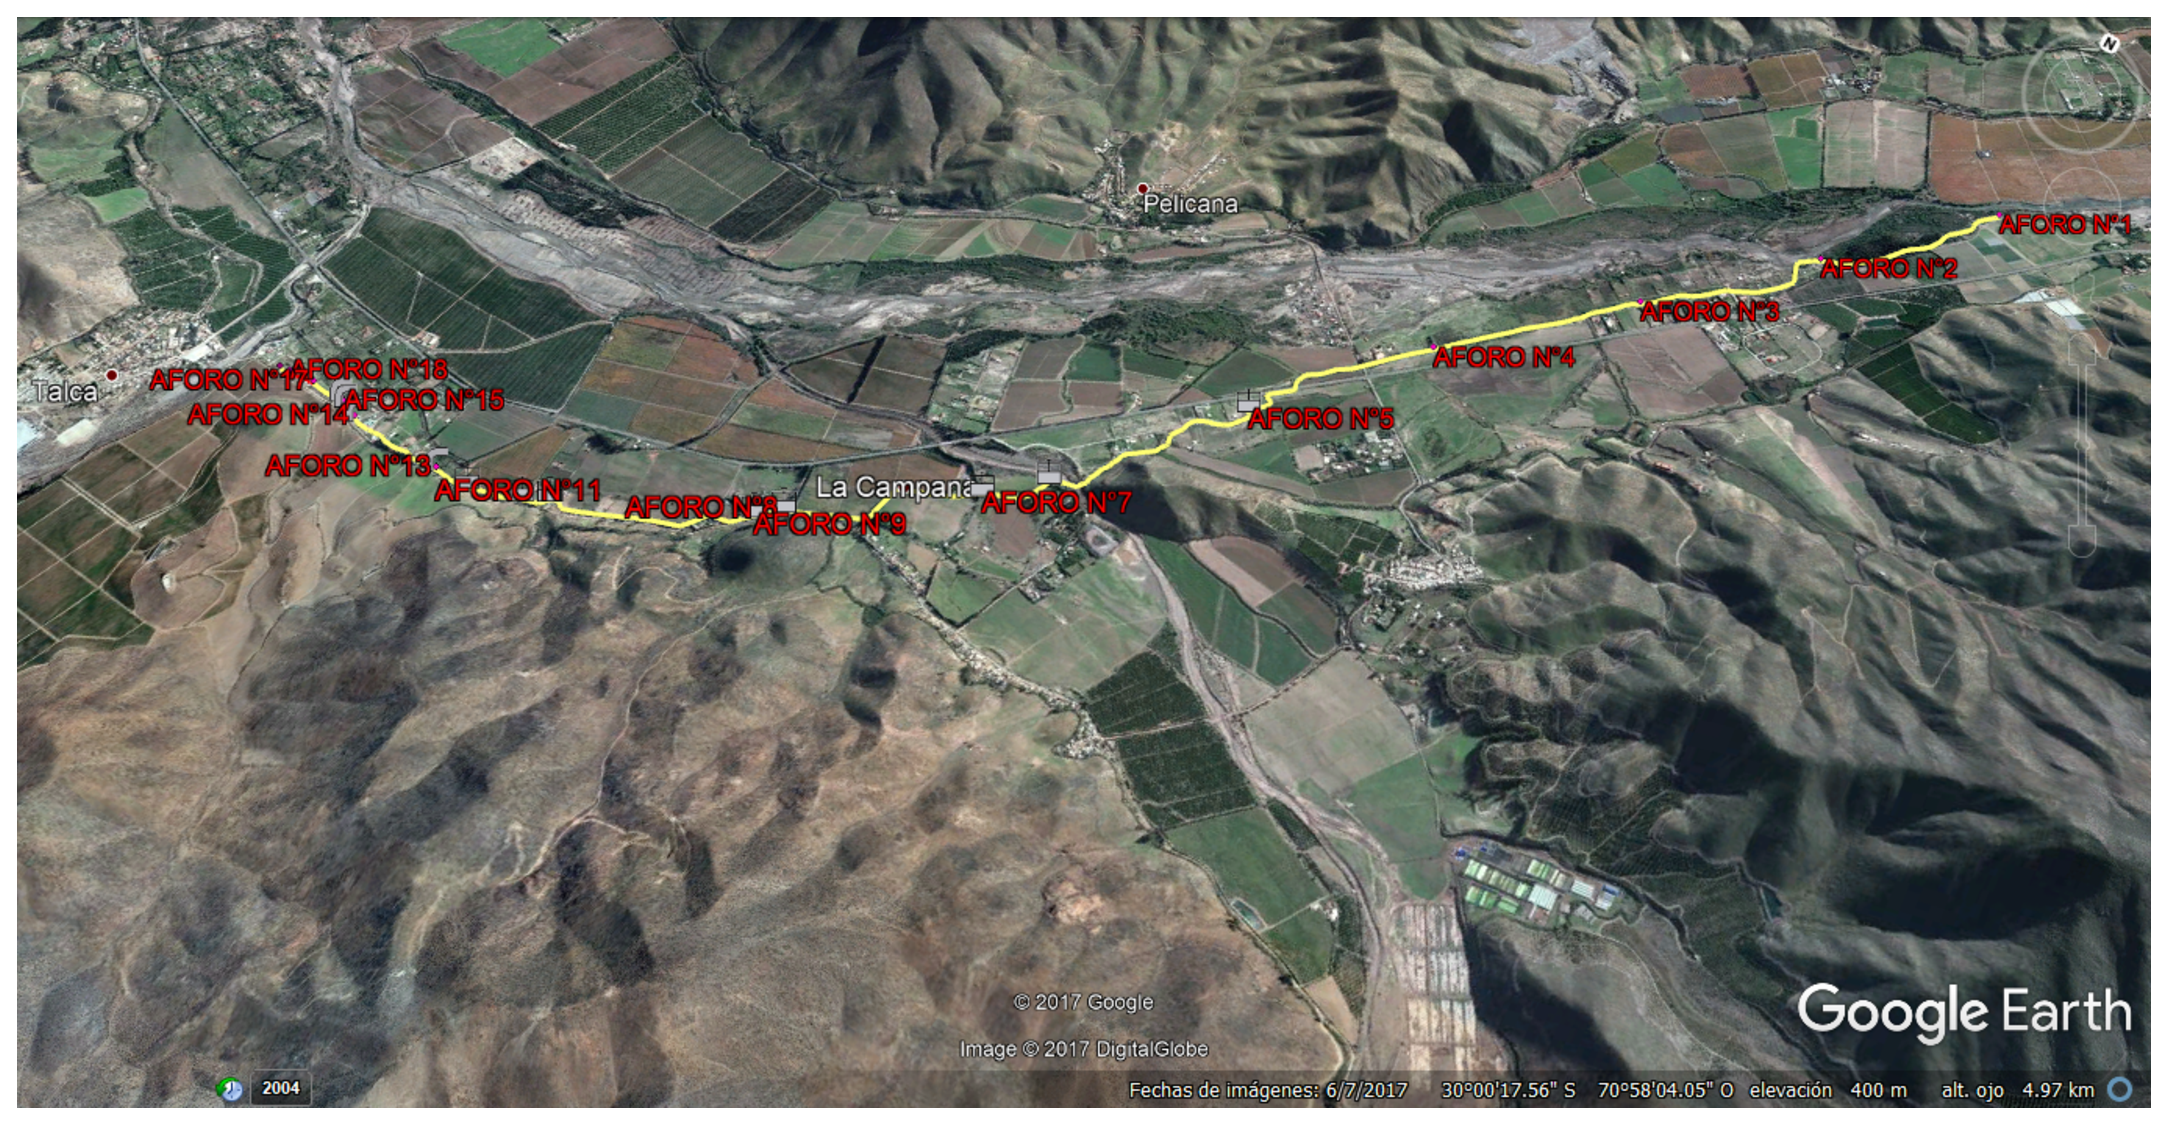
\includegraphics[width=\textwidth]{images/puntos_de_aforo_kml2.eps}
\caption{Archivo.kmz con trazado de canal y puntos de aforo. Ejemplo Canal Titón, JVRE.}
\label{kmz}
\end{figure}

\paragraph{Determinación de tramos:} Con la información de longitud, infraestructura y material de revestimientos presentes, se definen los tramos de aforo del canal. Estos se dividen por tipo de revestimientos, donde además se genera el tramo matriz, el cual se considera hasta la primera entrega. Estos tramos se generan para determinar las pérdidas generales por conducción del canal y/o tramo. Cada tramo consta de un aforo inicial y final, además de los posibles puntos de entregas o aportes que se puedan presentar y/o reglas operacionales del canal (turnos). Para la determinación de tramos, no se consideran cambios de revestimientos a los sectores del trazado que presenten una longitud menor a 0,1 $km$ y que se encuentren de forma intermedia en un mismo revestimiento, debido a que los aforos para la determinación de pérdidas pueden presentar alteraciones debido a la cercanía, y además permite operar de forma más eficiente.

\begin{table}[H]
\centering
\caption{Tramos del canal Titón (Junta de Vigilancia del Río Elqui y sus afluentes).}
\label{tramosE}
\begin{tabular}{|c|c|c|c|c|c|c|c|}
\hline
\textbf{Tramo}                         & \textbf{\begin{tabular}[c]{@{}c@{}}N°\\ aforo \\ inicial\end{tabular}} & \textbf{\begin{tabular}[c]{@{}c@{}}N°\\ aforo\\ final\end{tabular}} & \textbf{\begin{tabular}[c]{@{}c@{}}Km\\ inicial\end{tabular}} & \textbf{\begin{tabular}[c]{@{}c@{}}Km\\ final\end{tabular}} & \textbf{\begin{tabular}[c]{@{}c@{}}Longitud\\ (km)\end{tabular}} & \textbf{Revestimiento}                                     & \textbf{Hitos}                                                                                   \\ \hline
{\color[HTML]{FE0000} \textbf{Matriz}} & {\color[HTML]{FE0000} \textbf{1}}                                      & {\color[HTML]{FE0000} \textbf{5}}                                   & {\color[HTML]{FE0000} \textbf{0}}                             & {\color[HTML]{FE0000} \textbf{3,24}}                        & {\color[HTML]{FE0000} \textbf{3,24}}                             & {\color[HTML]{FE0000} \textbf{Mezcla suelo}}               & {\color[HTML]{FE0000} \textbf{\begin{tabular}[c]{@{}c@{}}Termino sección\\ Matriz\end{tabular}}} \\ \hline
\textbf{2}                             & 5                                                                      & 15                                                                  & 3,24                                                          & 6,91                                                        & 3,67                                                             & Mezcla suelo                                               & \begin{tabular}[c]{@{}c@{}}14 Comp y\\  5 Capt\end{tabular}                                      \\ \hline
\textbf{3}                             & 15                                                                     & 16                                                                  & 6,91                                                          & 6,94                                                        & 0,03                                                             & \begin{tabular}[c]{@{}c@{}}Hormigón - \\ Roca\end{tabular} & 1 Capt                                                                                           \\ \hline
\textbf{4}                             & 16                                                                     & 17                                                                  & 6,94                                                          & 7,07                                                        & 0,14                                                             & Mezcla suelo                                               & -                                                                                                \\ \hline
\textbf{5}                             & 17                                                                     & 18                                                                  & 7,07                                                          & 7,19                                                        & 0,11                                                             & PVC                                                        & -                                                                                                \\ \hline
\textbf{6}                             & 18                                                                     & 19                                                                  & 7,19                                                          & 7,24                                                        & 0,05                                                             & Mezcla suelo                                               & -                                                                                                \\ \hline
\end{tabular}
\end{table}
Una vez determinados los puntos de inicio y final del tramo, debemos realizar los aforos. Para cada punto, debemos seleccionar una sección de aforo, la que dependiendo de sus características, determinará el equipo de aforo que se utilizará.

\paragraph{Procedimiento de aforo con flujómetro:}
Previo a la ejecución del aforo, es necesario seleccionar la sección donde se va realizar la medición. Esta sección debe cumplir con ciertos requisitos técnicos y logísticos para obtener una medición confiable, dentro de lo que destaca la ubicación de esta, la que debe ser en un tramo recto del cauce, donde se aprecien líneas de flujo uniformes y paralelas a los márgenes de la corriente, con una pendiente longitudinal constante (evitar tramos con quiebres fuertes y áreas de aguas muertas, además de contracorrientes o remolinos). La base de la sección debe ser lo más regular posible, con un cauce estable y sin obstáculos o vegetación que interfieran, evitando lechos fangosos. La geología del terreno deberá facilitar, en caso de ser necesario, el acceso para construcción, medición y mantención de obras.\\
\\
Los aforos se realizan siguiendo el método de Área-Velocidad, el que consiste en la determinación del área de la sección transversal y la velocidad media del flujo de esta, obteniendo como producto el caudal pasante. El comienzo de la toma de datos, consiste en la medición del ancho total de la sección conductora, el que se obtiene mediante la medición de la distancia horizontal desde un punto de referencia ubicado en el plano de la sección transversal (espejo de agua). Con este ancho, se determina el número de subsecciones, el que está basado \emph{Manual Auto instructivo de aforo en canales no revestidos -- Ley Nº18.450} de la CNR y que se define por la siguiente fórmula:

\[{L} = \dfrac{T}{n} \]

donde:\\
\(n\): Número de subsecciones.\\
\(T\): Ancho superficial (m).

\begin{table}[H]
 \caption{Valores de \(n\)}
 \centering
 \begin{tabu} to 0.5\linewidth {>{\centering}X>{\centering}X}
 \toprule
 Ancho \(T\) (m) & \(n\)\\
 \midrule
 Menos de 1 m & 4 \\  
    1 - 2 m & 6 \\ 
    2 - 4 m & 10 \\  
    4 - 8 m & 16 \\ 
    8 - 10 m & 20 \\ 
    Más de 10 m & 24 \\ 
    \hline 
 \end{tabu}
\end{table}

Para la recolección de datos, se utiliza la planilla PROMMRA Q-CANAL, donde las subsecciones se determinan de forma automática al ingresar el ancho del canal; procediendo posteriormente a la determinación de la profundidad de cada subsección, lo que se realiza en la parte central de cada una, además de agregar la profundidad de ambos costados del cauce. Con esta información y a partir de la profundidad de las verticales (\(h_{w_s}\)), las mediciones son realizadas al 20\%, 60\% u 80\% de la profundidad de la vertical. Con esta información se genera dos tipos de valores; (1) La primera clasificación corresponde al valor de la altura desde la lámina de agua a la base del canal (del cual deriva el método tradicional de medición) y (2) el valor de altura desde la base a la lámina de agua, cuyo valor es más práctico en terreno.

\begin{table}[H]
 \caption{Alturas consideradas para la determinación de velocidad}
 \centering
 \begin{tabu} {cc}
 \toprule
 $h_{w_s}$ & Medida de velocidad en la subsección\\
 \midrule 
    $h_{w_s} \leq 0,2$ m & $0,6h_{w_s}$ \\ 
    $0,2$ m $< h_{w_s} \leq 0,5$ m  & $0,2h_{w_s}$; $0,6h_{w_s}$\\ 
    $h_{w_s} \geq 0,5$ m & $0,2h_{w_s}$; $0,6h_{w_s}$; $0,8h_{w_s}$\\
    \hline 
 \end{tabu}
\end{table}

Para la determinación del caudal, se utiliza un flujómetro de tipo electromagnético marca HACH modelo FH 950. Las velocidades determinadas por este equipo fueron ingresadas a la planilla de aforo (PROMMRA Q-Canal) con lo cual se obtuvo el caudal de forma inmediata. Además del caudal, la planilla entrega una gráfica con el perfil transversal de la sección aforada, así como la distribución de las velocidades.\\
\\
Finalmente se deberán seguir algunas consideraciones al realizar el aforo, entre las cuales tenemos:

\begin{itemize}
\tightlist
\item El molinete debe quedar completamente sumergido de forma de no incorporar distorsiones en la medida realizada.
\item El molinete debe colocarse de forma perpendicular a la sección de aforo, paralelo al escurrimiento de forma tal que mida la velocidad del punto.
\item Se deben tomar 3 medidas o repeticiones para determinar el valor de la velocidad en cada punto.
\item Es recomendable comenzar tomando las medidas en una vertical desde el fondo del canal.
\item Se debe comenzar el aforo desde el lado izquierdo del canal, observando este desde hacia aguas abajo.
\item La toma de medida en un punto, debe durar al menos 60 segundos, anotándose posteriormente la velocidad obtenida, en la hoja respectiva destinada para el aforo. Se considerará válido el promedio de 3 repeticiones por punto.
\end{itemize}

\paragraph{Procedimiento de aforo con trazador químico:}

La medición de caudal mediante este método está basada en la determinación del grado de dilución en el agua de una sustancia trazadora y como esta modifica la conductividad eléctrica del flujo a medir. Este método permite conocer el caudal a partir de la variación de concentración de una sustancia que es inyectada en el flujo. Este tipo de aforo se recomienda para canales con láminas de agua de poca profundidad (menor a 10 cm), de sección irregular, con flujo turbulento, pendientes importantes, lechos inestables y líneas de flujo desordenadas, donde los métodos tradicionales de aforo no son aplicables.\\
\\
El criterio principal para definir el emplazamiento, donde se lleva a cabo la determinación de caudal mediante el empleo de este método, es que en ese punto se produzca una mezcla homogénea de la solución inyectada en un tramo relativamente corto del canal. La mezcla del trazador con el flujo, se ve potenciada con las rugosidades propias del canal y la presencia de piedras o cantos, los cuales aumentan la turbulencia de la corriente.

\begin{itemize}
\tightlist
\item Como regla general se recomienda comenzar la medición en la variación de la conductividad eléctrica, desde el punto final del tramo a evaluar hacia atrás, es decir devolviéndose por el canal. Con esto se evita que restos de sales de mediciones anteriores pudiesen interferir al momento de una nueva determinación de la conductividad eléctrica y por ende afectar en la determinación del caudal.
\item A modo referencial, la cantidad de trazador a utilizar para determinar caudal se estima en 10 g de trazador por cada l/s de caudal. Para estimar el caudal pasante se puede utilizar el método de aforo con flotador.
\item Se deberá determinar la distancia (L) entre el punto de inyección y el punto de medición, la cual se puede obtener mediante la siguiente expresión:

\[L=0,13*C+\left(\frac{(0.7*C)+6}{g}\right)*\frac{b^2}{d}\]

donde:\\
\(b\): Ancho medio del canal.\\
\(d\): Profundidad media del flujo.\\
\(C\): Coeficiente de Chezy para el tramo $(15<C<50)$.\\
\(g\): Aceleración de gravedad.\\
El coeficiente de Chezy $(C)$, puede determinarse con la siguiente expresión:

\[C=\left(\frac{1}{n}*R^\frac{1}{6}\right)\]

donde:\\
\(n\): Rugosidad del canal (Manning).\\
\(R\): Radio hidráulico de la sección (área/perímetro).\\
En caso de no conocer los valores del coeficiente de Manning (n), así como la pendiente
del tramo a evaluar se recomienda la utilización de la siguiente expresión:

\[L=2*v*\frac{b^2}{d}\]

donde:\\
\(L\): Distancia para la dilución del trazador ($m$).\\
\(v\): Velocidad media ($m/s$).\\
\(b\): Ancho medio del canal ($m$).\\
\(d\): Profundidad media del flujo ($m$).\\
\item Se debe medir la conductividad eléctrica inicial del flujo ($C_0$), registrar dicha información.
\item Medición de la temperatura del flujo y registro de su valor. Se registra esta información para efectuar el ajuste necesario de la CE (a 20°$C$) de manera de poder comparar mediciones, realizadas bajo distintas condiciones de temperatura.
\item Este procedimiento se debe repetir 3 veces por punto de medición, para obtener una lectura confiable.
\end{itemize}

\paragraph{Planilla PROMMRA Q- Canal:} La planilla de cálculo de caudal (Figura \ref{q_canal}), se utiliza para recolectar los datos del aforo con flujómetro. Presenta dos secciones, la primera (sector superior) describe la planilla en términos generales y presenta celdas para ingresar información general; mientras que la segunda sección (sector inferior), posee las celdas para el ingreso de los datos de aforo y además presenta los resultados de cálculo.

%insertar figura de planilla q-canal.
\begin{figure}[H]
\centering
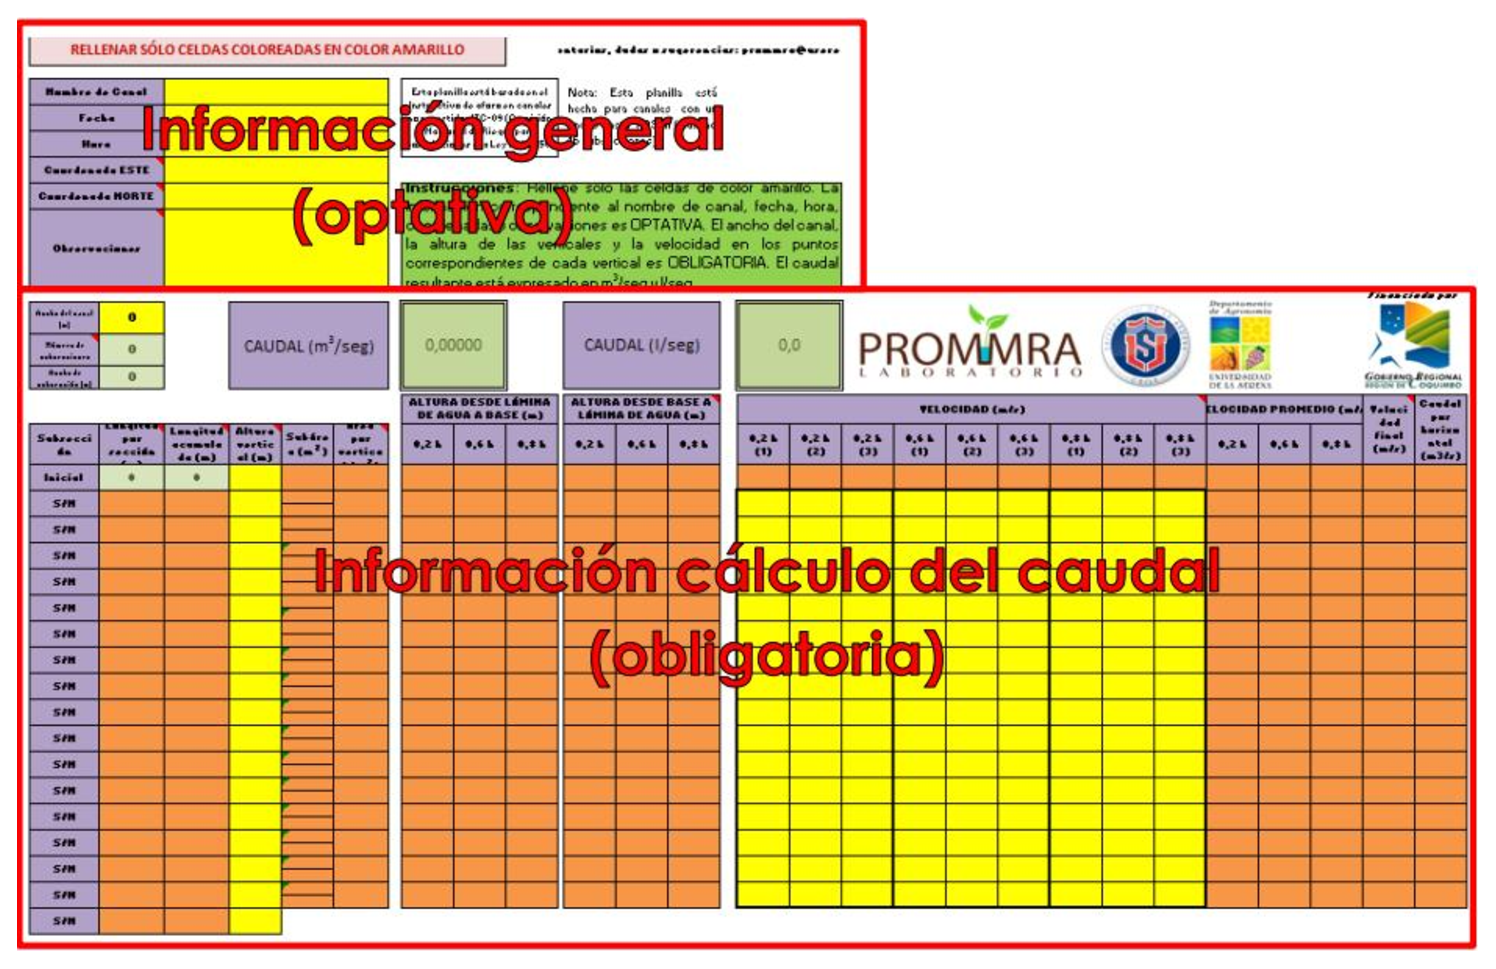
\includegraphics[width=0.7\textwidth]{images/planilla_qcanal.eps}
\caption{Vista general planilla de aforo (Q-Canal).}
\label{q_canal}
\end{figure}

\subparagraph{Información general:}
En esta sección se informa al usuario de las instrucciones y potencialidades de la planilla (Figura \ref{info_general}). También existe la posibilidad de ingresar los datos generales del punto de aforo, como nombre del canal, fecha, hora, ubicación (coordenadas) y observaciones. Es recomendable completar dicha información para la caracterización del punto de aforo además de tener un respaldo para el seguimiento de dicho punto.

%insertar figura informacion general.
\begin{figure}[H]
\centering
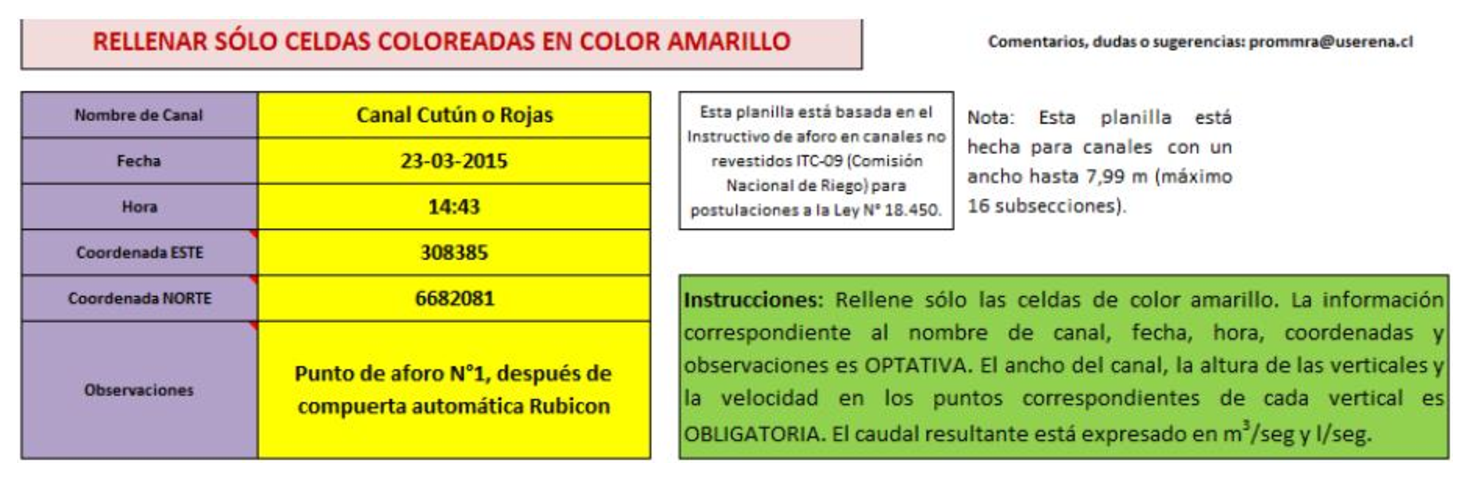
\includegraphics[width=0.7\textwidth]{images/info_general.eps}
\caption{Sección información general, planilla Q-Canal.}
\label{info_general}
\end{figure}

\subparagraph{Sección información cálculo de caudal.}
El primer dato que se debe ingresar en esta sección es el ancho del canal (en metros). Una vez realizada esta acción, automáticamente se calculara el número de subsecciones y el ancho de cada subsección. Además, se completaran las columnas de “Longitud por sección (m) y “longitud acumulada (m)” (Figura \ref{casilla}).

%insertar figura numero subsecciones.
\begin{figure}[H]
\centering
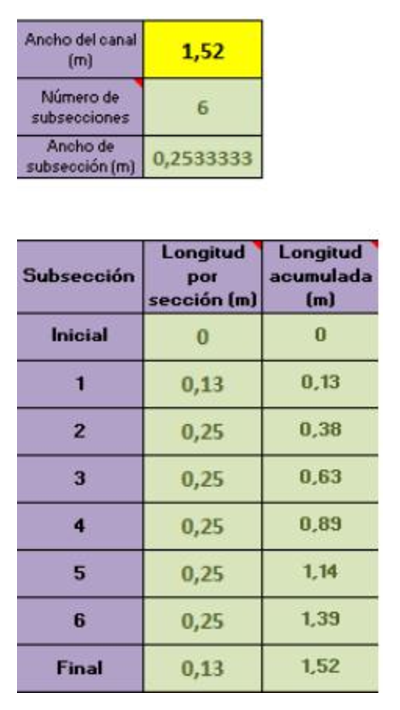
\includegraphics[width=0.2\textwidth]{images/n_subsecciones.eps}
\caption{Número de subsecciones y ubicación dentro de la sección de aforo. Ejemplo: ancho sección de aforo 1,52 m (casilla amarilla).}
\label{casilla}
\end{figure}

Luego es necesario ingresar el valor de profundidad vertical en cada subsección. Este dato es utilizado para determinar el número de puntos por vertical para determinar velocidad (figura \ref{pto_vert}). Además se presentan los valores de profundidad en la cual se debe medir cada una de estas velocidades. Este valor de profundidad se presenta en dos formatos, el primero es el que se utiliza convencionalmente para el cálculo de dichos puntos, el cual va desde la lámina de agua hacia la base o fondo, mientras que el segundo utiliza el cálculo realizado con el primer formato pero los valores se expresan desde la base del canal a la lámina de agua. Este último valor es más práctico a la hora de determinar los puntos en terreno. Finalmente, el valor de la altura por vertical, en conjunto con los determinados anteriormente, permite el cálculo del área por vertical (dato usado para la determinación de caudal por subsección). 

%insertar figura puntos vertical.
\begin{figure}[H]
\centering
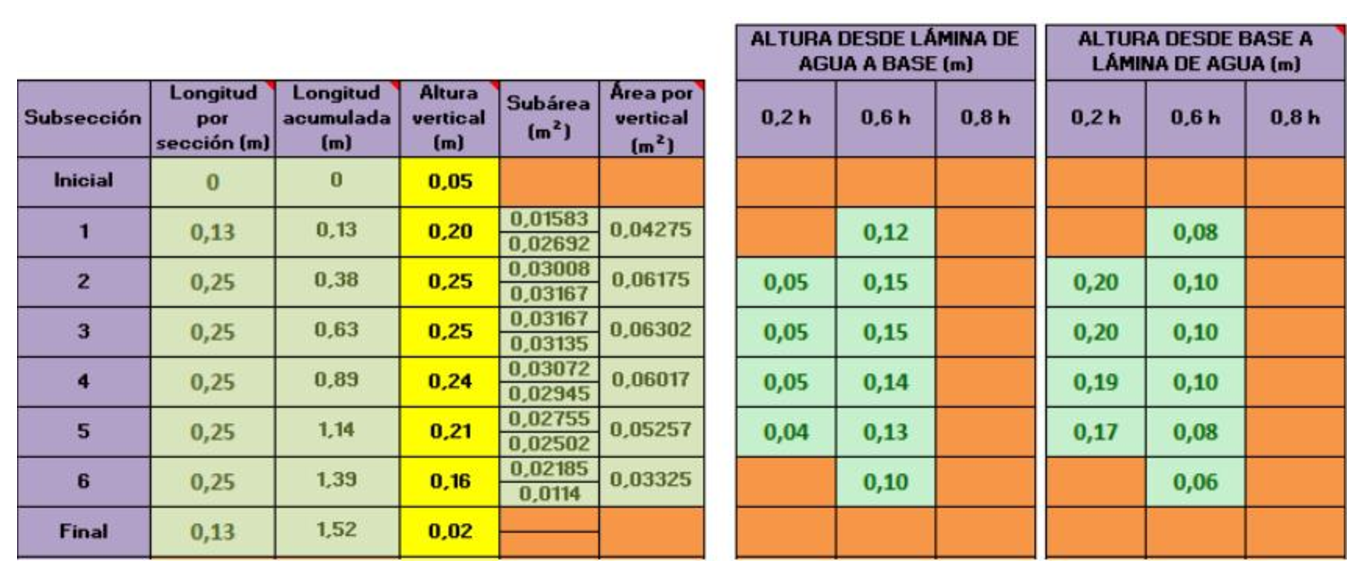
\includegraphics[width=0.7\textwidth]{images/puntos_vertical.eps}
\caption{numero de mediciones de velocidad por vertical, en función de la profundidad de cada una de estas.}
\label{pto_vert}
\end{figure}

La planilla entrega la posibilidad de ingresar 3 valores de velocidad diferentes por cada punto de medición por vertical (Figura \ref{ing_veloc}). Estos valores se promedian para ser utilizados en el cálculo de la velocidad final por subsección.

%Insertar figura velocidad vertical
 \begin{figure}[H]
\centering
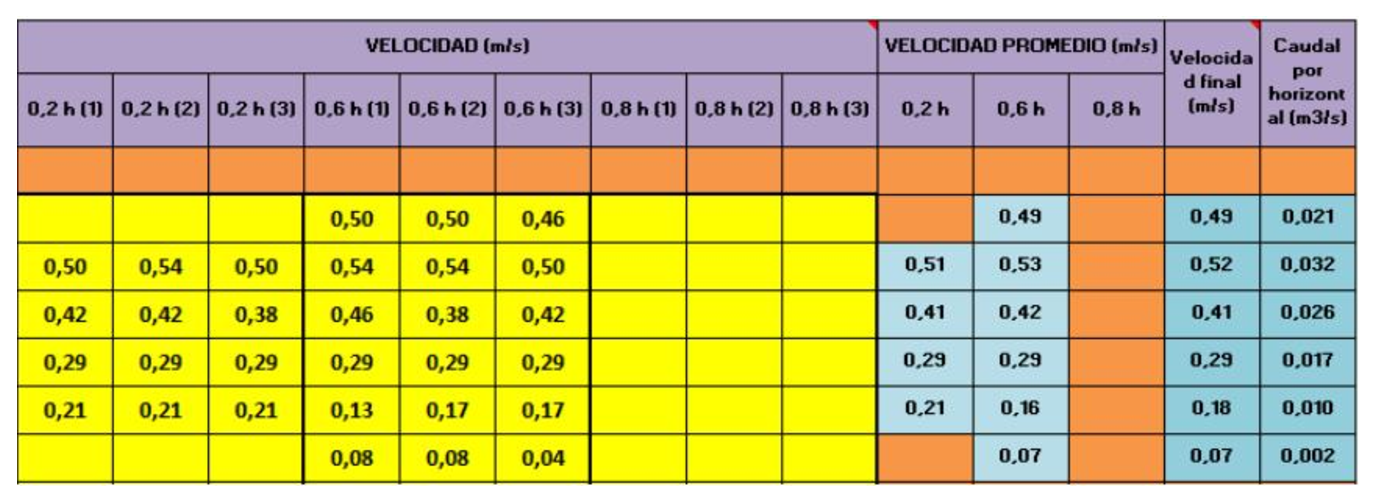
\includegraphics[width=0.7\textwidth]{images/ingreso_veloc.eps}
\caption{Ingreso de velocidad por punto de aforo en la vertical.}
\label{ing_veloc}
\end{figure}

La velocidad por subsección se calcula utilizando los algoritmos presentados en el instructivo ITC-09 de la Comisión Nacional de Riego. Esta velocidad es multiplicada por el área de la subsección para determinar el caudal en esta. La sumatoria de los caudales en las diferentes subsecciones determina el caudal final del punto de aforo. Este caudal se expresa en $m^3$/s y l/s (Figura \ref{res_q}).\\

%insertar figura de caudal
\begin{figure}[H]
\centering
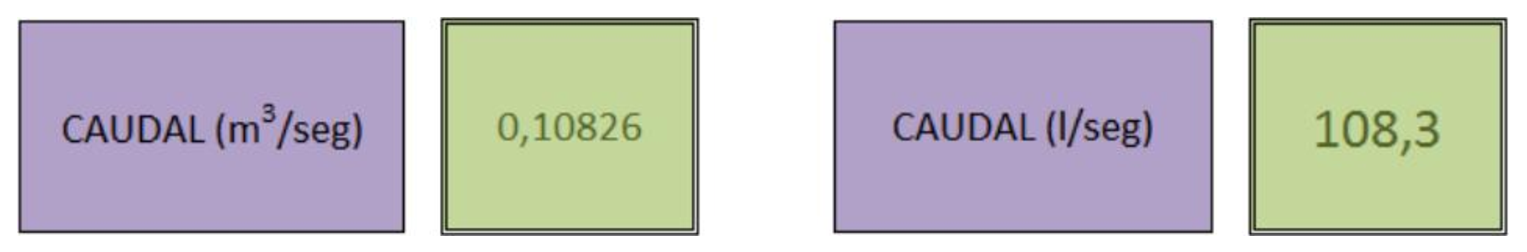
\includegraphics[width=0.7\textwidth]{images/caudal.eps}
\caption{Resultados de caudal, expresados en dos unidades de medición.}
\label{res_q}
\end{figure}

Se debe recordar que la planilla Q-Canal, solo utiliza los valores de las celdas indicadas para el cálculo de velocidad y en caso de que falte algún dato de velocidad, se indicara el mensaje “FALTAN DATOS” (Figura \ref{faltan_d}). Esto asegura el uso correcto de los valores ingresados en la planilla y alerta al usuario de falla en el ingreso de datos.\\

%insertar figura faltan datos
\begin{figure}[H]
\centering
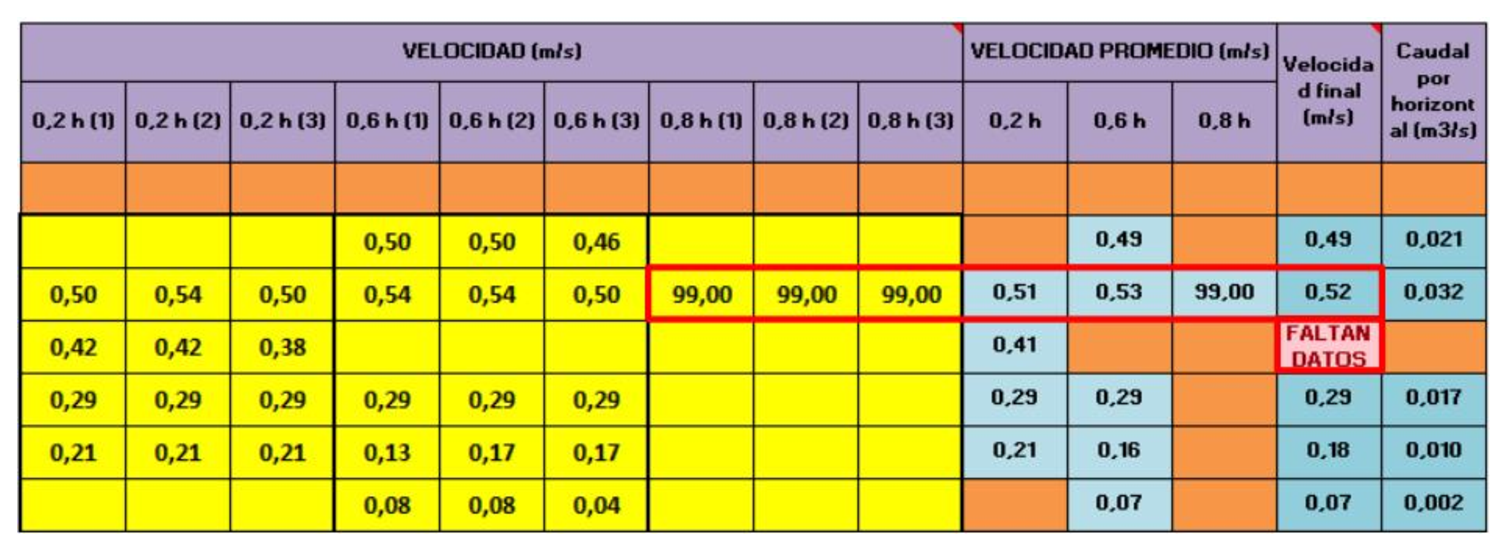
\includegraphics[width=0.7\textwidth]{images/faltan_datos.eps}
\caption{Ejemplo del comportamiento de la planilla por ingreso erróneo o falta de datos.}
\label{faltan_d}
\end{figure}

Además se incorporó una sección que mediante colores representa las velocidades a lo ancho el canal (Figura \ref{dist_veloc}). El objetivo de este cuadro es identificar el comportamiento del flujo en el perfil transversal del punto de aforo. El resultado representado en el cuadro permite corroborar si la sección de foro se encuentra emplazada correctamente. 

%insertar figura velocidad perfil transversal
\begin{figure}[H]
\centering
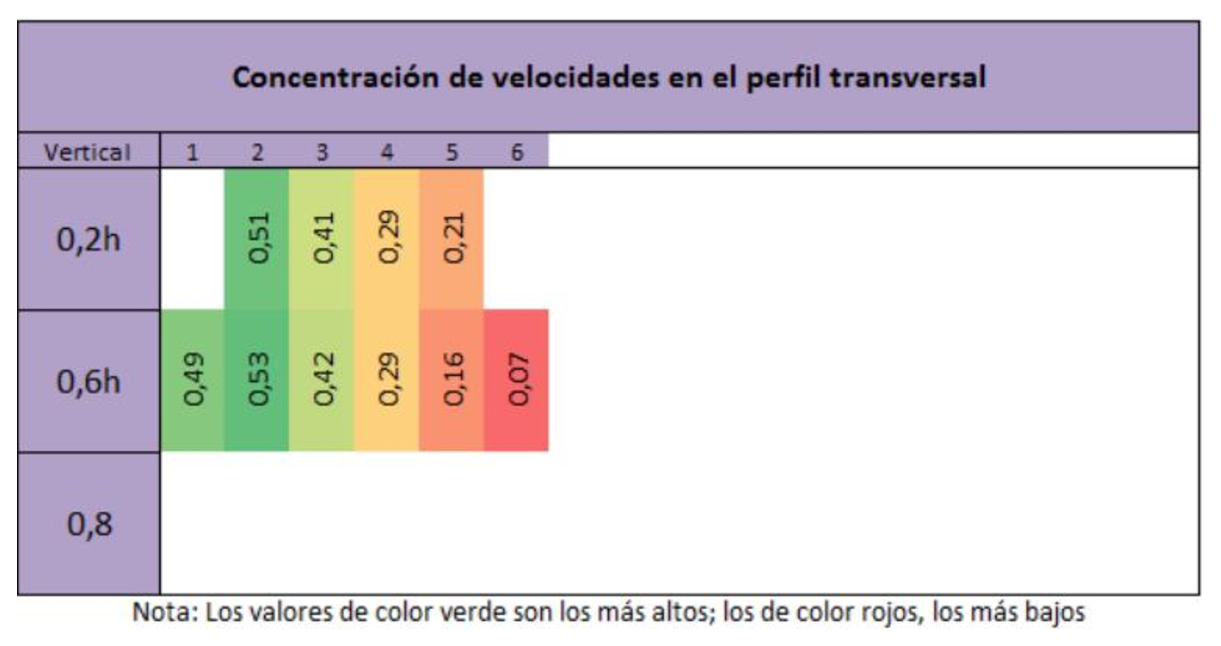
\includegraphics[width=0.7\textwidth]{images/perfil_tran.eps}
\caption{Distribución de velocidades en el perfil transversal.}
\label{dist_veloc}
\end{figure}

Otra de las opciones que incorpora esta planilla corresponde  a una hoja de cálculo denominada “Gráfico Perfil Canal”. En ella se gráfica automáticamente el perfil transversal del canal, a partir de los valores de ancho del canal y altura de cada vertical (Figura \ref{graf_esq}). Dicho gráfico tiene como objetivo dar a conocer a quien afora de las irregularidades en el fondo del canal.

%insertar figura grafico perfil transversal canal
\begin{figure}[H]
\centering
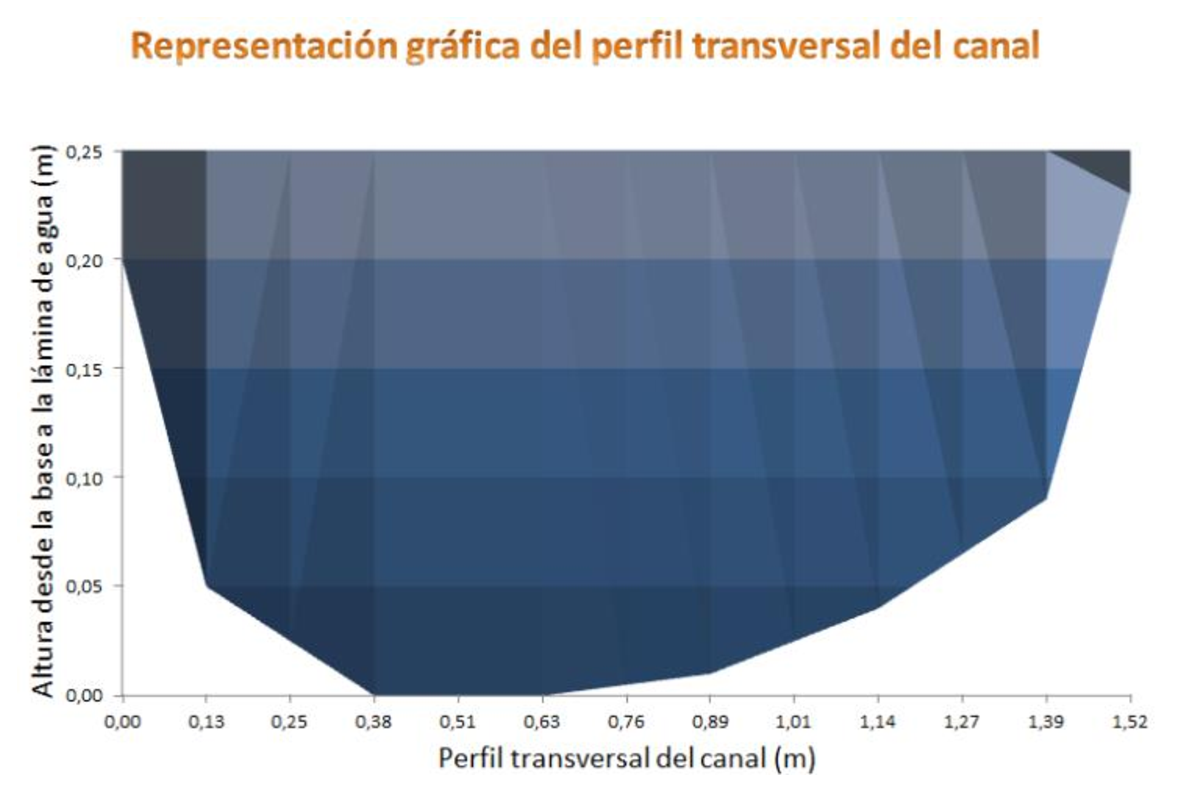
\includegraphics[width=0.7\textwidth]{images/grafico_esquematico.eps}
\caption{Gráfico esquemático del perfil transversal del canal.}
\label{graf_esq}
\end{figure}

\paragraph{Determinación de pérdidas por conducción en tramos y canales:} Existen dos instancias donde se determinan pérdidas, dependiendo del elemento que se esté evaluando, vale decir tramos (a nivel individual) o canales (como sumatoria de los tramos que lo componen). Cada uno de estos elementos es evaluado en instancias diferentes, siendo los tramos evaluados en terreno mientras se ejecutan las labores de aforo. En el caso de la evaluación general de pérdidas del canal esta labor es efectuada en gabinete, y con la totalidad de información de cada uno de los tramos que lo componen.\\
\\
La evaluación de terreno se realiza por cada tramo, para el cual se utiliza la capa KMZ (Figura \ref{kmz}) más la información asociada con el detalle de cada uno de los puntos y tramos para evaluación de pérdidas (Cuadro \ref{tramosE}). Se realizan los aforos inicial y final del tramo, junto con las posibles entregas o aportes que se encuentren en ese momento. Las entregas o aportes encontrados en el tramo pueden ser determinadas directamente o indirectamente. La determinación directa, consiste en el aforo directo en la compuerta predial de existir las condiciones hidráulicas. La determinación indirecta consiste en la medición del caudal antes y después de la compuerta de entrega o aporte, la diferencia entre ambas mediciones corresponderá al agua entrante o saliente al canal. Cuando existen salidas o aportes en el tramo, el caudal final se considera como teórico, el que considera las entregas o aportes dentro del tramo, por lo cual, este caudal representa el volumen de agua que debiese conducir el tramo del canal en una situación sin salidas o aportes, permitiendo comprar de mejor forma el caudal inicial del tramo con el evaluado en la parte final, para lo cual se utiliza la siguiente ecuación:

\begin{equation}
Q Teorico (l/s) = Q Real + \sum{Caudal Entregas Prediales o Aportes}
\end{equation}

En función de la diferencia entre el caudal inicial y final, se decidirá subdividir el tramo evaluado para una nueva determinación de pérdidas.  Si la diferencia entre ambos caudales es superior al 20$\%$, y además este tramo es de una extensión superior a 1 km, será necesario subdividir el tramo en partes iguales, generándose los sub-tramos. Siguiendo el procedimiento se aforará en el punto medio, si la diferencia entre este caudal y los definidos  anteriormente (inicial o final, en función del tramo analizado) es superior al 20$\%$, se deberá hacer una nueva subdivisión siempre y cuando la extensión del sub-tramo evaluado supere la longitud de 1 km, de caso contrario la evaluación queda circunscrita al sub-tramo original. Para definir las pérdidas en terreno del tramo analizado, se utiliza la siguiente fórmula:

\begin{equation}
Perdidas Tramo (\%)=\frac{(Q_i - Q_f)}{(Q_i)}*100
\end{equation}

donde:\\
$Q_i$: Caudal inicial (l/s)\\
$Q_f$: Caudal final (l/s)\\

Para comprender de mejor manera la subdivisión de tramos, a continuación se presenta un ejemplo y el procedimiento en cada caso. El tramo presenta una longitud de 3,2 km y un caudal inicial de 100 l/s.\\

\textbf{Situación 1.} Perdidas del tramo general menor al 20\%. En este caso las pérdidas corresponden al 12\%, por lo cual no se hace necesaria una nueva división del tramo (Figura \ref{sit_1}).

%insertar figura situacion 1 
\begin{figure}[H]
\centering
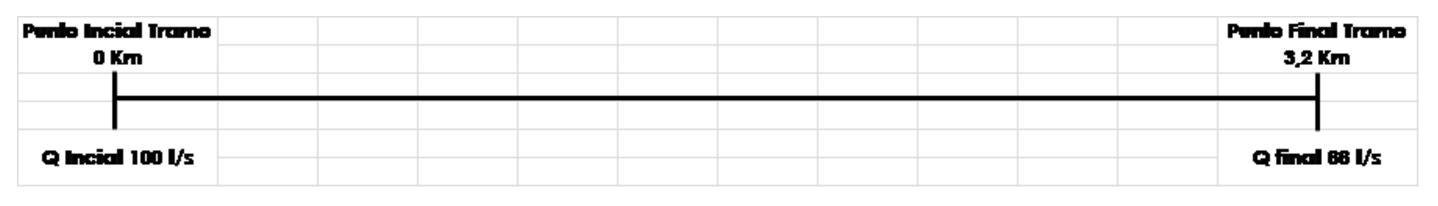
\includegraphics[width=0.7\textwidth]{images/sit_1.eps}
\caption{Tramo con pérdidas menores al 20\%}
\label{sit_1}
\end{figure}

\textbf{Situación 2.} Pérdidas tramo general superiores al 20\%. En este caso las pérdidas corresponden al 25\%, lo cual significa que se debiese subdividir el tramo original, además la extensión del tramo aforado es de 3,2 km (Figura \ref{sit_2}), por lo cual se cumplen las dos condiciones que justifican la subdivisión de un tramo. De esta manera el tramo original se divide en partes iguales, vale decir a los 1,6 km (Figura \ref{sit_2_1}).

\begin{figure}[H]
\centering
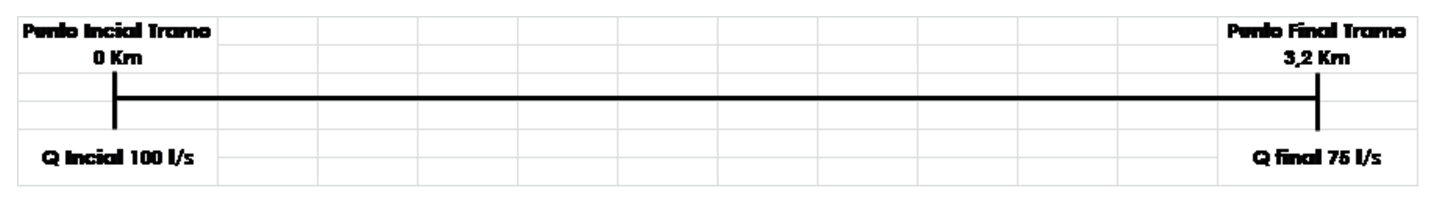
\includegraphics[width=0.7\textwidth]{images/sit_2.eps}
\caption{Tramo con pérdidas mayores al 20\%}
\label{sit_2}
\end{figure}

\begin{figure}[H]
\centering
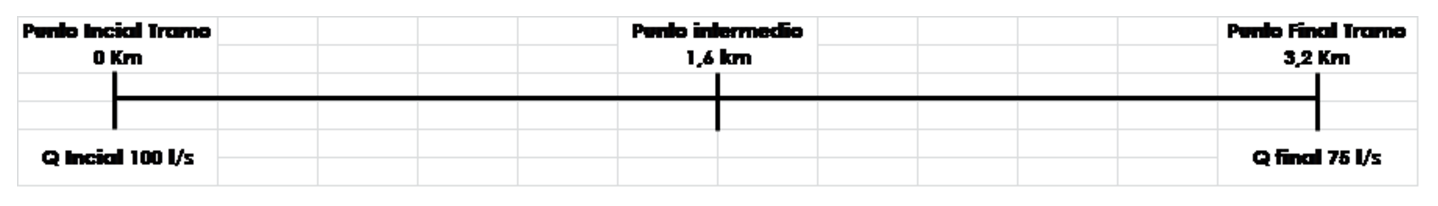
\includegraphics[width=0.7\textwidth]{images/sit_2_1.eps}
\caption{Tramo con pérdidas mayores al 20\% y subdivisión a los 1,6 km.}
\label{sit_2_1}
\end{figure}

\textbf{Situación 3.} La división del tramo original y aforo correspondiente, arrojan pérdidas en los nuevos sub-tramos inferiores al 20\% (Figura \ref{sit_3}). De esta manera al no registrar pérdidas superiores al límite establecido, no se continúa dividiendo el tramo original.\\

\begin{figure}[H]
\centering
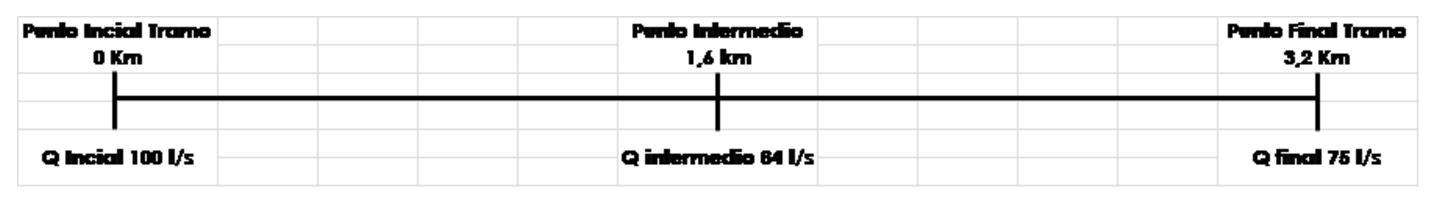
\includegraphics[width=0.7\textwidth]{images/sit_3.eps}
\caption{Subdivisión tramo general y caudal punto intermedio.}
\label{sit_3}
\end{figure}

Como podemos apreciar en la Figura \ref{sit_3}, se crean 2 nuevos tramos, el primero que va desde el kilómetro 0 a 1,6 presenta caudales de 100 l/s y 84 l/s, por lo tanto pérdidas del 16\%, no requiere nueva subdivisión (Figura \ref{sit_3_1}). El segundo tramo va desde el kilómetro 1,6 al 3,2, presentando caudales de 84 l/s y 75 l/s, por lo tanto pérdidas del 11\% (Figura \ref{sit_3_2}), de igual manera este tramo no se continúa subdividiendo.\\

\begin{figure}[H]
\centering
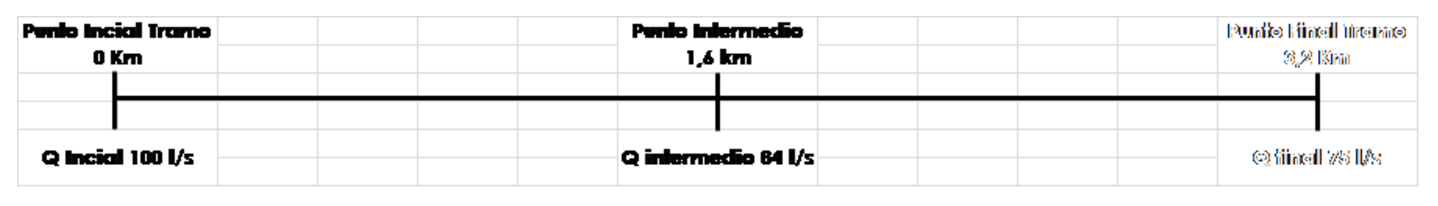
\includegraphics[width=0.7\textwidth]{images/sit_3_1.eps}
\caption{Caudal inicial y final, tramo km 0 - 1,6.}
\label{sit_3_1}
\end{figure}

\begin{figure}[H]
\centering
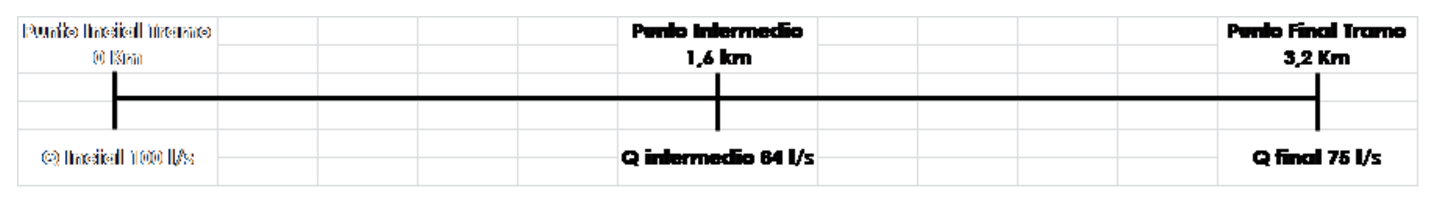
\includegraphics[width=0.7\textwidth]{images/sit_3_2.eps}
\caption{Caudal inicial y final, tramo km 1,6 - 3,2.}
\label{sit_3_2}
\end{figure}

\textbf{Situación 4.} La división del tramo general original y aforo correspondiente indican que las pérdidas en uno de los nuevos tramos es superior al 20\% (Figura \ref{sit_4}). En este caso el tramo comprendido entre los 1,6 km y 3,2 presenta caudales que varían entre 96 l/s y 75 l/s.\\

\begin{figure}[H]
\centering
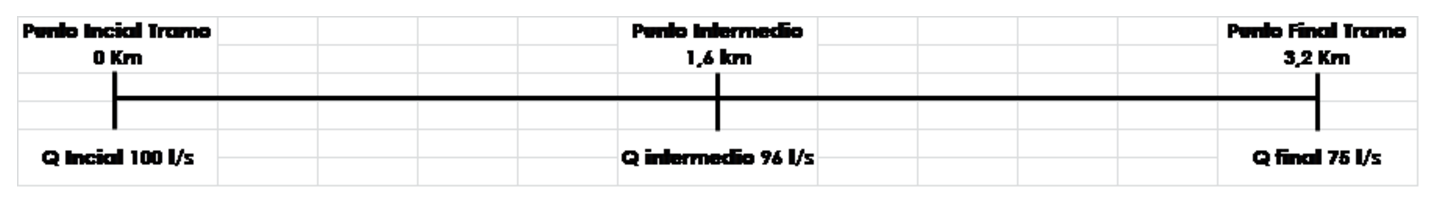
\includegraphics[width=0.7\textwidth]{images/sit_4.eps}
\caption{Tramo subdividido, genera subtramos (2), donde uno de los dos presenta pérdidas mayores al 20\%.}
\label{sit_4}
\end{figure}

De esta manera el tramo entre el kilómetro 1,6 y 3,2 presentan una perdida equivalente al 21,9\%, por lo cual este tramo debería ser nuevamente dividido ya que su longitud supera 1 km (Figura \ref{sit_4_1}).\\

\begin{figure}[H]
\centering
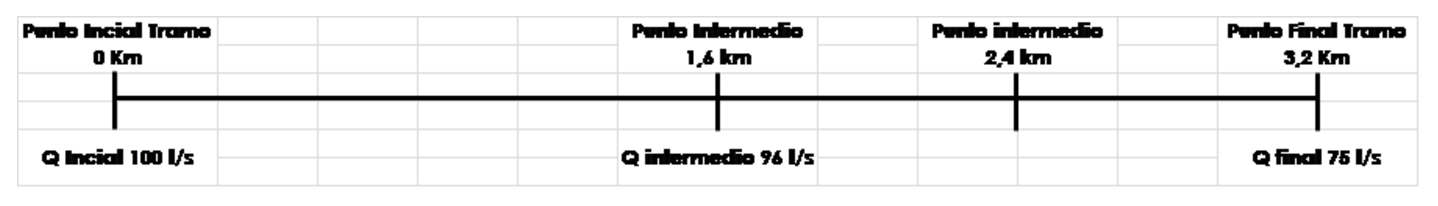
\includegraphics[width=0.7\textwidth]{images/sit_4_1.eps}
\caption{Subtramo dividido nuevamente, por pérdidas superiores al 20\%.}
\label{sit_4_1}
\end{figure}

\textbf{Situación 5}. Sub-tramo (situación 4) presenta pérdidas mayores al 20\%. Por tratarse de una división de un sub-tramo de 1,6 kilómetros, esta nueva segmentación genera tramos de 0,8 km de longitud, por lo cual solo hasta ese punto se subdivide el tramo original, y se da por finalizado el proceso de aforo de este tramo originalmente de 3,2 km (Figura \ref{sit_5}) .\\

\begin{figure}[H]
\centering
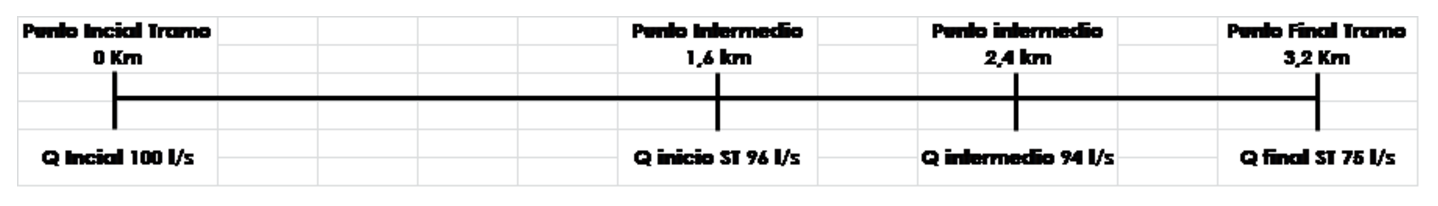
\includegraphics[width=0.7\textwidth]{images/sit_5.eps}
\caption{Subtramo (situación 4), presenta una diferencia de entre caudal inicial y final superior al 20\%.}
\label{sit_5}
\end{figure}

Una vez determinadas las pérdidas de todos los tramos, en el trabajo de gabinete, se procede a tabular los datos de caudales iniciales, entregas o aportes y finales aforados en los tramos y subtramos en que fue dividido el canal, junto con la longitud definida. Las pérdidas determinadas se expresan en litros por segundo ($l/s$), en porcentaje del volumen ($\%$), pérdidas en litros por kilómetro ($l/km$) y pérdidas en porcentaje por kilómetro ($\%/km$) para cada tramo.

\begin{equation}
Perdidas (l/s) = Q Inicial Tramo - Q Final Teorico Tramo 
\end{equation}

\begin{equation}
Perdidas (\%) = \frac{Q Inicial Tramo (l/s)}{ Q Final Teorico Tramo (l/s)} * 100
\end{equation}

\begin{equation}
Perdidas (l/km) = \frac{Perdidas (l/s)}{Longitud Del Tramo (km)}
\end{equation}

\begin{equation}
Perdidas (\%/km) = \frac{Perdidas (l/s)}{Longitud Del Tramo (km)}
\end{equation}

Una vez tabulados los datos de pérdidas por tramo, se procede a determinar la pérdida general del canal, aplicando el porcentaje de pérdidas correspondiente de cada tramo o subtramo al caudal de inicio del canal. El caudal incial ($QInicial$) es sometido a todos los porcentajes de pérdidas correspondientes a cada tramo de dicho canal. Al aplicar el primer porcentaje de pérdidas, el caudal resultante ($QFinaltramo \textup{ n }$), se considera como caudal final para aplicar el próximo porcentaje de pérdidas. Una vez aplicados todos los porcentajes de pérdidas de los tramos o subtramos del canal, el resultado es transformado en porcentaje obteniendo la pérdida general del canal.

\begin{equation}
 \begin{split}
	Perdidas generales(\%) & = 100-[[Q Incial (l/s) - [Q Inicial (l/s) * Perdidas Tramo \textup{ 1 } (\%)/100]\\
	&\quad - Q Final Tramo \textup{ 1 } (l/s) * Perdidas Tramo \textup{ 2 } (\%)/100\\
	&\quad - Q Final Tramo \textup{ 2 } (l/s) * Perdidas Tramo \textup{ n } (\%)/100 \\
	&\quad - Q Final Tramo \textup{ n } (l/s) * Perdidas Tramo \textup{ n+1 } (\%)/100]\\
	&\quad * 100 / Q Inicial (l/s)]
 \end{split}
\end{equation}

La información obtenida en la Determinación de pérdidas en conjunto con la recopilada en el S.I.G., nos permite generar las variables de volumen recuperado por temporada y Volumen recuperado por temporada en función de longitud de mejoramiento.

\begin{itemize}
\item \textbf{Volumen recuperado por canal} ($m^3/temporada$ y $m^3/m^2$)
\end{itemize}

Con la información obtenida en las etapas anteriores, se procedió a desarrollar una matriz de análisis para la determinación de la recuperación general ($m^3/temporada$) y recuperación por valor unitario de revestimiento ($m^3/m^2 de revestido$) por temporada para cada uno de los tramos con revestimiento no permanente de los canales. Las variables incluidas son las siguientes:

\begin{itemize}
\item Pérdidas generales: corresponde a la diferencia entre el caudal de inicio y caudal final registrado en el canal. Dicho valor solo considerará los tramos sin revestimiento permanente. La determinación de esta variable requiere la reconstrucción de caudal, en caso de que los aforos que permitieron estimar las pérdidas del canal fuesen hechos en distintas fechas o se registraran entregas y/o aportes. Las pérdidas de caudal serán expresadas en ($l/s$).
\item Longitud general afecta a mejoramiento ($m$): corresponde a la extensión del canal que no presenta revestimiento permanente, y que por ende está en condiciones de entrar en el proceso de priorización.
\item Dimensiones a revestir: corresponde al ancho y alto de la sección transversal del canal que se utiliza como base para revestimientos, es decir, condiciones de revestimiento rectangular. Las dimensiones se expresan en ($m$).
\item Recuperación general canal: corresponde al volumen generado producto de un mejoramiento de la totalidad del trazado del canal (considera solo segmentos sin revestimiento permanente). Esta variable será expresada $m^3/temporada$. Para la determinación de esta variable se utiliza la siguiente expresión:

\begin{equation}
Recuperacion general(m^3/temporada)= \frac{Perdidas generales (l/s) * 60 seg. * 60 min. * 24 hrs. * 365 dias} {1000}  
\end{equation}

\item Superficie a revestir canal general: como su nombre lo indica corresponde al área afecta a revestimiento y que considera el ancho y alto de las paredes del canal, además de la longitud de los tramos a mejorar. Esta variable será expresada en $m^2derevestido$ y será determinada utilizando la siguiente expresión:

\begin{equation}
\begin{split}
	Superficie a revestir (m^2)& = Ancho (m) * Longitud a revestir (m)\\
	&\quad + 2 * Alto (m) * Longitud a revestir (m)  
\end{split}
\end{equation}

Recuperación general por unidad revestida ($m^3/m^2 de revestido$): corresponde al volumen recuperado por metro cuadrado de mejoramiento (considera solo segmentos sin revestimiento permanente) por temporada. La determinación de esta variable se hará con la siguiente expresión:

\begin{equation}
m^3/m^2 de revestido = \frac{m^3/temporada} {m^2 de revestido}  
\end{equation}

\end{itemize}
Una vez recopilada toda la información de las diferentes etapas, se procede a realizar la priorización de canales y/o tramos bajo la siguiente metodología.

\subsubsection{Priorización de canales y/o tramos.}

Las variables requeridas e insumos para generar variables, necesarios en la aplicación del Protocolo de priorización de inversiones en mejoramiento de la eficiencia de conducción hídrica, se seleccionaron a través de un análisis de correlación PEARSON realizado a la sistematización o matriz inicial de análisis con toda la información recabada de la red hídrica perteneciente a la OUA's, en relación a la variable pérdidas generales por conducción ($l/s$), debido a que el plan de priorización tiene como objetivo aumentar la eficiencia de conducción hídrica. Se aplica el análisis de correlación PEARSON, en un software como Statgraphics, Statsoft, Minitab, R, SSPS o similares, donde se determina que las variables requeridas e insumos para generar variables, se correlacionaban en más de un 80$\%$.\\
\\
La ejecución del Protocolo de priorización de inversiones en mejoramiento de la eficiencia de conducción hídrica, se realiza a través de una sistematización de la información o matriz de análisis, de la cual se excluyen bocatomas que no corresponde a canales como las captaciones, además de canales con información incompleta, canales con pérdidas generales igual a 0\% o con recuperaciones de agua y los canales revestidos en su totalidad. El protocolo de priorización está orientado solo a aquellos tramos de canales que no presentan revestimientos de tipo permanente, es decir, sin revestimientos (mezcla de suelo) y revestidos con geomembrana (temporal), los cuales pueden ser postulados a fondos de la ley de Riego principalmente.\\
\\
Una vez determinadas estas variables e insumos,se ejecuta un análisis de árbol de decisión (clasificación), con el fin de conformar grupos de canales que sean similares y puedan competir entre sí. La matriz se compone de las siguientes variables e insumos:

\begin{itemize}
\item \textbf{Longitud total del canal en uso ($km$):} Dice relación la longitud actual del canal que efectivamente se está utilizando y que no necesariamente corresponde a la longitud del trazado original del canal. Este factor es esencial para determinar la superficie afecta a mejoramiento del canal ($m^2$ a revestir).
\item \textbf{Longitud tramo matriz ($km$):} Corresponde a la distancia entre la compuerta que da origen al canal y la primera entrega predial. Es imprescindible contar con esta información, ya que, permite estimar superficie de este tramo afecta a mejoramiento. Cabe recordar que cualquier mejora en este tramo, beneficia a la totalidad de los usuarios del canal.
\item \textbf{Longitud tramo matriz a revestir ($km$)}: corresponde a la extensión del canal compuesta desde la compuerta que da origen al canal y la primera entrega predial que se encuentra sin revestimiento de tipo permanente.
\item \textbf{Longitud afecta a revestimiento ($km$):} corresponde a la extensión del canal que no presenta revestimiento permanente y por ende está en condiciones de ser sometida a mejoramiento.
\item \textbf{Dimensiones de la sección afecta a revestimiento:} Se relaciona a factores tales como ancho y alto de los tramos que se pretenden mejorar, con esta información se puede determinar un valor estimativo de $m^2$ de revestimiento necesarios para el mejoramiento.
\item \textbf{Pérdidas generales por conducción ($l/s$):} El agua que se utiliza para el riego, llega a los cultivos después de recorrer un conjunto de canalizaciones desde la fuente de abastecimiento. Durante ese recorrido se producen pérdidas que hacen que la cantidad de agua que realmente llega hasta el predio sea muy inferior a la disponible en la iniciación del sistema de irrigación.
\item \textbf{Pérdidas tramo matriz ($l/s$):} corresponde a la diferencia de caudal entre el volumen determinado en la compuerta que da origen al canal y la primera entrega predial.
\item \textbf{Pérdidas tramo distribución ($l/s$):} corresponde a la diferencia de caudal existente entre el volumen medido en la primera y última entrega predial del canal.
\item \textbf{Área y longitud a revestir:} Conocer el área y longitud de un canal, es de vital importancia al momento de generar una mejora en su sistema de conducción, ya que en función de estos dos parámetros se puede calcular el costo de inversión de la obra de mejoramiento.
\end{itemize}

Una vez determinados los grupos de canales, se procede a realizar una verificación de la clasificación, para la cual se utiliza un análisis de tipo discriminante que permite asignar o clasificar nuevos individuos u observaciones dentro de grupos o segmentos previamente definidos. Con los grupos conformados y ratificados, se procede a realizar ordenamiento decreciente de las variables requeridas, informadas en el inicio de la revisión, esto nos entregará un orden para cada una, las que se promediarán, obteniendo la jerarquización final de los canales y/o tramos.

\subsubsection{Diagnóstico y propuesta de fortalecimiento}

El protocolo de priorización de inversiones en mejoramiento de la eficiencia de conducción hídrica generado en SIMCA-ELQUI, según el diagnóstico efectuado, estableció que la base o fundamentos para la priorización son parámetros del ámbito técnico principalmente, por lo que la incorporación de nuevos parámetros, y fuentes de información, permitirá un fortalecimiento de esta herramienta con el fin de establecer un desarrollo equitativo y sustentable de la cuenca. Además se evidenció la falta de información a nivel de Comunidades de aguas, los principales entendidos del trazado y área de influencia asociada a ésta, y uno de los beneficiarios directos de la generación del Plan de priorización.\\
\\
Para potenciar esta herramienta, se crea una propuesta de fortalecimiento que incluye un nuevo nivel de recopilación de información, específicamente a las Comunidades de aguas, desarrollo de nueva metodología de recolección de la variable superficie regada, inclusión de parámetros del ámbito social, como determinación del área de influencia de la Comunidad de aguas y la Modelación hidrológica de la cuenca.\\
\\
Las Comunidades de aguas, son las encargadas de administrar el recurso hídrico y además son los principales entendidos en el área de influencia de ésta, por lo que resulta fundamental incorporar información de estas. Para recopilar esta información se realizará una entrevista a un representante, con el fin de conocer detalladamente el trazado y singularidades del canal, junto con generar una línea base del área de influencia ligado a este. Los antecedentes propuestos para realizar la entrevista son los siguientes:

\begin{itemize}
\item Número de acciones y litros/segundo
\item Número de usuarios
\item Longitud canal ($km$)
\item Número de entregas
\item Número de ramales
\item Capacidad de porteo canal ($l/s$)
\item Manejo operacional (secciones)
\item Tipos y porcentajes de revestimientos
\item Superficie regada por há
\item Principales cultivos
\item Sistemas de riego empleados ($\%$)
\item Descarga final al río
\end{itemize}

Junto con estos antecedentes, es necesario individualizar la Comunidad de aguas, Nombre representante y su cargo, además de registrar contactos y fecha de entrevista.\\
\\
La nueva metodología de recopilación de antecedentes de la superficie regada, será a través de un levantamiento en terreno con el fin de actualizar esta información. La inclusión de nuevas variables se enfocará en el ámbito social, con lo cual se busca fomentar la permanencia de la población en el sector, crear o potenciar polos productivos y mejorar la calidad de vida a través de la creación de nuevos empleos. Se realiza en primera instancia a través del área de influencia de las Comunidades de aguas, la que estará ligada a la superficie bajo riego y potencial, y posteriormente mediante una modelación hidrológica de la cuenca, con el objetivo de evitar efectos negativos en la disponibilidad de recursos de otras zonas. El detalle de la inclusión de estás variables se presenta en los siguientes apartados.\\
\\
Dentro de la priorización, esta se realizará en primera instancia solo a los canales, para posteriormente realizar una priorización de los tramos que lo componen. La priorización a nivel de canales contempla la inclusión de las variables de ordenamiento de superficie bajo riego y potencial, además de la variable modelamiento hidrológico. La priorización de los tramos dentro del canal se realizará a través de las variables de volumen recuperado por temporada y por unidad, junto con la superficie bajo riego y potencial asociada a este.\\
\\
El fortalecimiento de esta herramienta dará origen al nuevo Protocolo técnico-social de inversión en mejoramiento de la eficiencia de conducción hídrica.

\subsection{Componente 1. Actividad 1.2. Definición parámetros y generación de los protocolos de variable superficie bajo riego y potencial.}

Como parámetros de superficie ligados al recurso hídrico, se establecen la superficie bajo riego y potencial. La primera corresponde a la que se encuentra cultivada en el período del proyecto, y la segunda, a la totalidad de la superficie cultiva o no cultivada al momento del proyecto. Para el levantamiento de esta información se generó el siguiente protocolo.

\subsubsection{Protocolo de las variables superficie bajo riego y superficie potencial.}

La superficie de cada variable se obtiene del Proyecto FIC-R Coquimbo 2015 \textit{``Generación e implementación de un programa de seguimiento y monitoreo de suelo agrícola para el ordenamiento del territorio"} (PROMUS), con algunas modificaciones en los polígonos representantes de superficie agrícola, entendiendo el constante seguimiento y actualización del dinamismo del uso agrícola en la región.\\
\\
La variable superficie bajo riego o cultivada corresponde al resultado de la clasificación de uso de suelo agrícola generada por PROMUS, donde cada uno de estos polígonos representa una clase de cultivo mediante clasificación de imágenes satelitales (frutales caducos, frutales persistentes, cultivos de ciclo corto, praderas, cultivos bajo plástico y la clase sin cultivo). Esta metodología de generación de esta variable se diferencia de la superficie cultivada obtenida en SIMCA-ELQUI, ya que aquella se obtuvo a través de recopilación de información.\\
\\
La variable superficie potencial se define como toda la superficie que haya sido o esta actualmente cultivada, esta superficie se obtuvo realizando polígonos que representan cuarteles o superficie de suelo erosionada mediante agricultura, que a través de imágenes satelitales fue posible detectar.\\
\\
Para conocer la superficie asociada a cada canal que será sometido a la priorización. En primera instancia, durante el trabajo de gabinete, con la capa de canales obtenidas de la CNR, a través del recorrido de estos, se asigno los polígonos que se encuentran mas próximos al trazado de este, los que se encuentran bajo cota del canal, en el caso de existir polígonos sobre canales este queda sujeto al trazado del canal más próximo.

\begin{figure}[H]
\centering
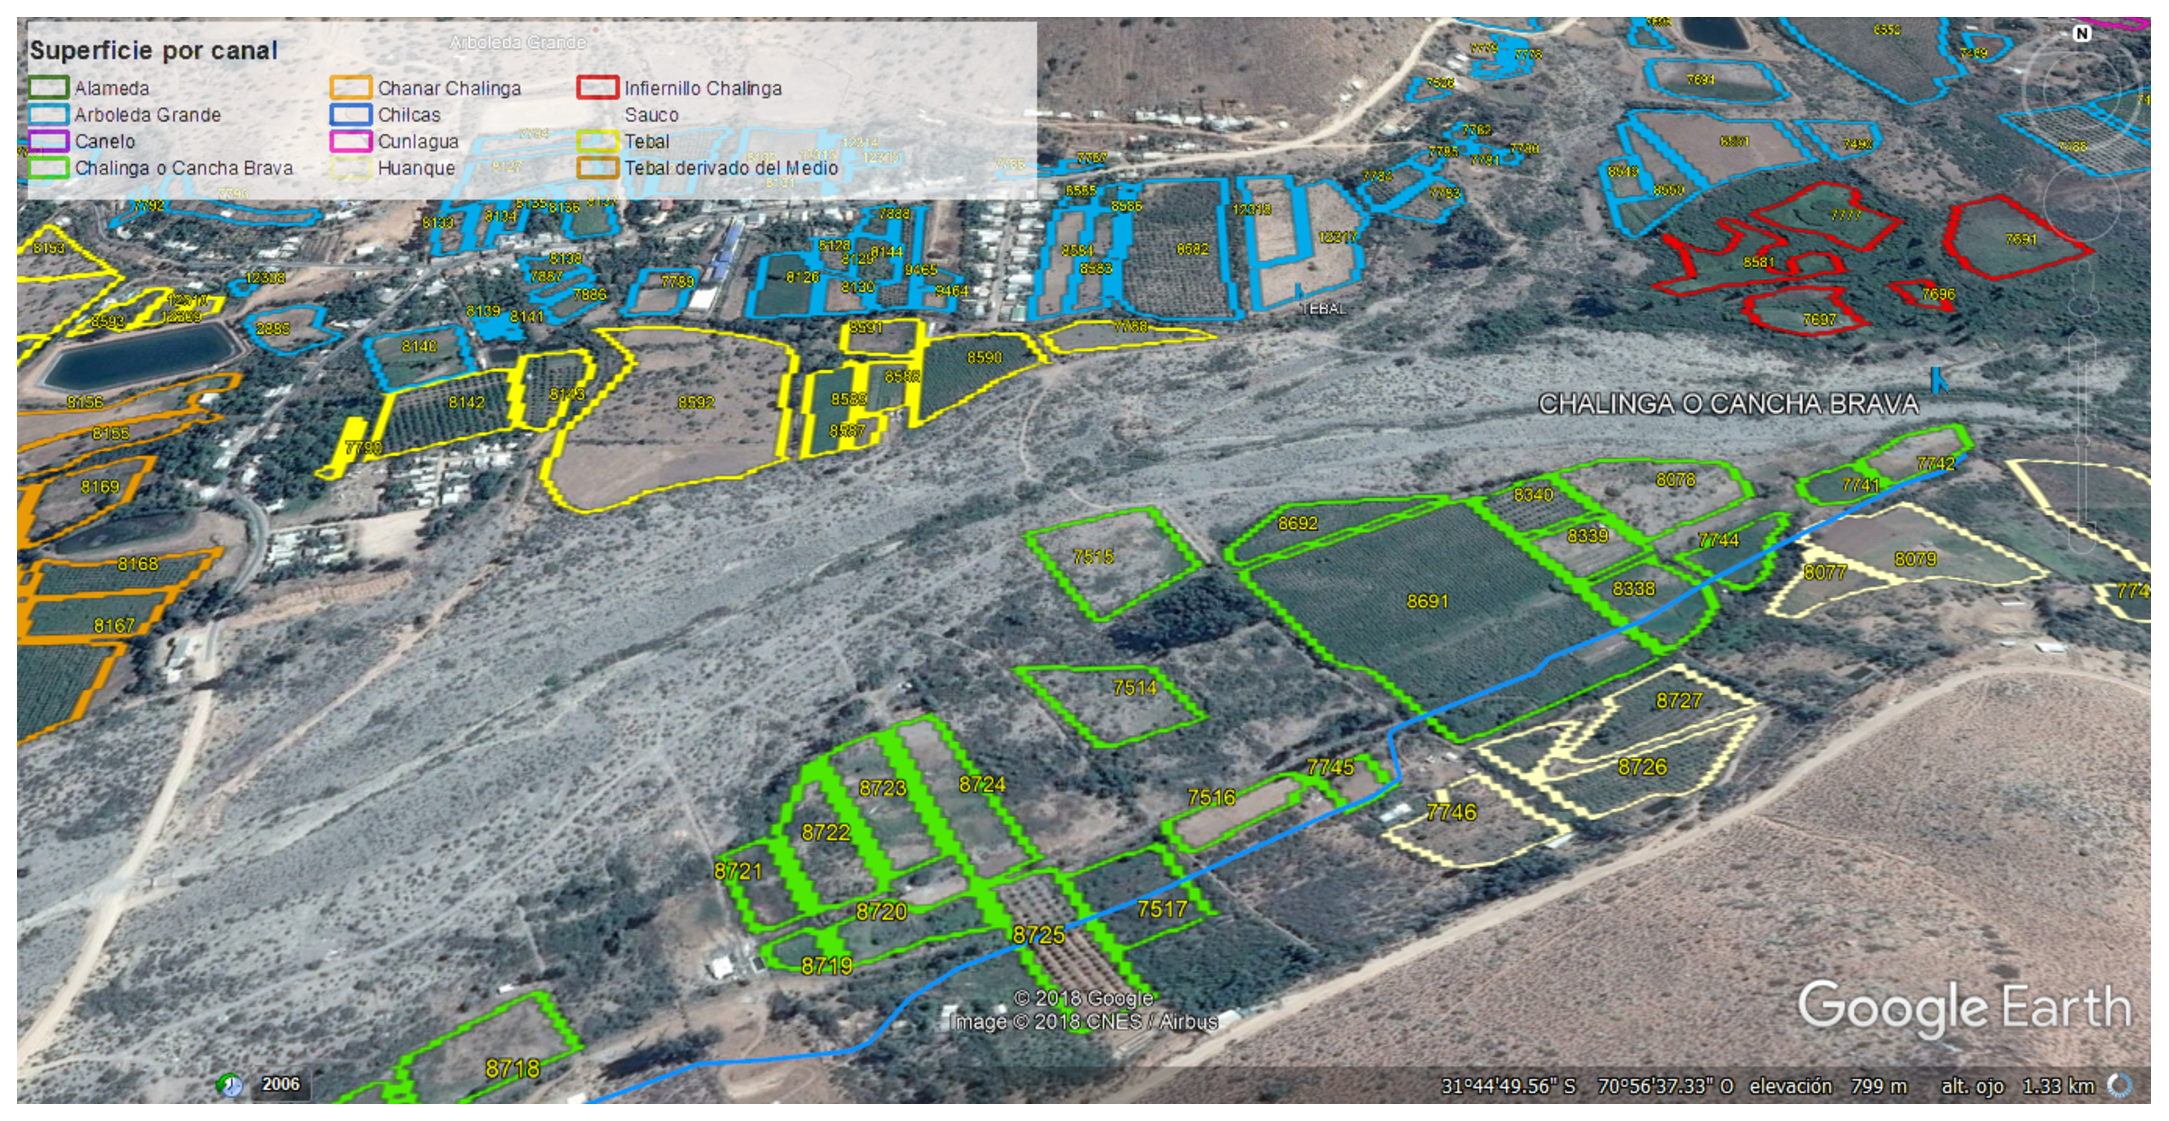
\includegraphics[width=\textwidth]{images/capa_kmz_area.eps}
\caption{Capa.kmz con polígonos y trazado de canal. Ejemplo trazado canal Cancha brava (línea celeste) y polígonos asociados a su recorrido (polígonos verdes)}
\label{poligonos}
\end{figure}

Una vez asignados los polígonos que representan la superficie de cada canal, durante las campañas de terreno, se procede a realizar entrevistas con representantes de cada canal, con el fin de acotar la superficie ligada a cada canal, además de realizar el levantamiento de información de cada polígono asociado al trazado de cada canal, la que se realiza mediante observación y registro en planillas con los polígonos asignados. La información recolectada es la siguiente:

\begin{itemize}
	\item \textbf{Superficie bajo riego}
	\begin{itemize}	
		\item Número ID
		\item Cultivo
		\item Especie
		\item Variedad
		\item Sistema de riego
		\item Observaciones
	\end{itemize}
	\item \textbf{Superficie potencial}
	\begin{itemize}	
		\item Número ID
		\item Sin Cultivo
		\item Observación
	\end{itemize}
\end{itemize}

Esta es la información básica para las variables superfice bajo riego y superficie potencial. La superficie asociada a cada variable se integra al protocolo mediante generación de nuevos ordenamientos que serán promediados junto a las variables requeridas. Además esta información nos permitirá ajustar la variable modelación hidrológica, a través de la determinación de demandas de cada zona o cultivo.

\subsection{Componente 1. Actividad 1.3. Definición de parámetros y generación de los protocolos para la variable modelamiento hidrológico.}

A partir de la modelación de escenarios de revestimiento zonificados en las distintas organizaciones de regantes, se establecieron 5 parámetros que el modelo WEAP entrega a partir de sus resultados, para evaluar los efectos hidrológicos en la cuenca. Tales parámetros se detallan a continuación.

\begin{enumerate}

\item \textit{Volumen almacenado en los embalses}. Se evaluará la condición de los volúmenes almacenados a lo largo de la serie temporal, a partir del escenario base con su condición histórica. A partir de este parámetro, se considerará como efecto negativo la disminución del volumen almacenado en la serie temporal, producto de una menor disponibilidad en la asignación para las siguientes temporadas, y viceversa.

El indicador es el porcentaje de disminución o aumento del volumen almacenado 	como promedio de la serie modelada en el escenario con revestimiento, respecto 	al escenario base.


\item \textit{Volumen almacenado en los acuíferos de la zona de influencia}. Se evaluará la dinámica de los volúmenes almacenados en los acuíferos que se encuentren en el área de influencia de los canales, considerando como efecto negativo, una disminución en su almacenamiento a lo largo de la serie temporal, y viceversa. Esto, debido a la menor disponibilidad hídrica para demandas que se abastecen de esta fuente de agua, sobretodo en periodos de escasez hídrica.

El indicador es el porcentaje de disminución o aumento del volumen almacenado 	como promedio de la serie modelada en el escenario con revestimiento, respecto 	al escenario base.

\item \textit{Caudales superficiales}. Se evaluará el comportamiento de los cauces naturales en puntos establecidos de la cuenca, con el fin de evidenciar la dinámica a lo largo de la serie temporal. Se considerará como efecto negativo, la disminución de los caudales a lo largo de la serie, debido a la disminución de la oferta hídrica en la asignación de la temporada, y viceversa.
	
El indicador es el porcentaje de disminución o aumento del caudal superficial como promedio de la serie modelada en el escenario con revestimiento, respecto al escenario base.


\item \textit{Satisfacción de la demanda agrícola}.Se evaluará el porcentaje de la cobertura de la demanda agrícola, tanto de los cultivos frutales, como cultivos anuales. En ambos casos, se considerará como efecto positivo, el aumento de la satisfacción de la demanda a lo largo de la serie temporal, y viceversa.

El indicador es el porcentaje de disminución o aumento de la cobertura de la 	demanda en el escenario con revestimiento, respecto al escenario base.


\item \textit{Seguridad de la cobertura de la demanda agrícola}.Se evaluará el porcentaje de la cobertura de la demanda agrícola, tanto de los cultivos frutales, como cultivos anuales. En ambos casos, se considerará como efecto positivo, el aumento de la satisfacción de la demanda a lo largo de la serie temporal, y viceversa.

El indicador es el porcentaje de disminución o aumento de la cobertura de la 	demanda en el escenario con revestimiento, respecto al escenario base.

\end{enumerate}

El protocolo de la variable modelación hidrológica, consiste en evaluar los parámetros ya establecidos bajo escenarios de revestimiento de canales zonificados en las tres áreas de influencia de cada organización, Junta de Vigilancia del río Chalinga y sus Afluentes; Junta de Vigilancia del río Choapa y sus Afluentes; y Junta de Vigilancia del río Illapel y sus Afluentes. Cada escenario de revestimiento será contrastado con un escenario base, el cual cuenta con una serie temporal entre 1990 – 2016, y detalla la situación histórica ocurrida en la cuenca.

Para la generación de estos escenarios de revestimiento, se debe disponer de información de cada comunidad, que permita contrastar la información utilizada en el modelo para su verificación. A continuación, se mencionan la información necesaria a verificar y el proceso de actualización.

\begin{itemize}

\item \textbf{\textit{Diagrama unifilar de los canales de cada organización}:} Dicha información permitirá verificar la zonificación de los canales y su correspondiente agrupación dentro del modelo respecto a: área de influencia de riego, ubicación y distribución dentro de la cuenca.

En el modeo WEAP de la cuenca del río Choapa, es posible verificar la agrupación de canales establecidas en la topología, estás son flechas de color naranjo llamadas \textit{“Diversion”}. En la figura \ref{etiqueta_figura3}, se observa la topología establecida para la modelación de la cuenca.


\begin{figure}[H]
\begin{center}
\fbox{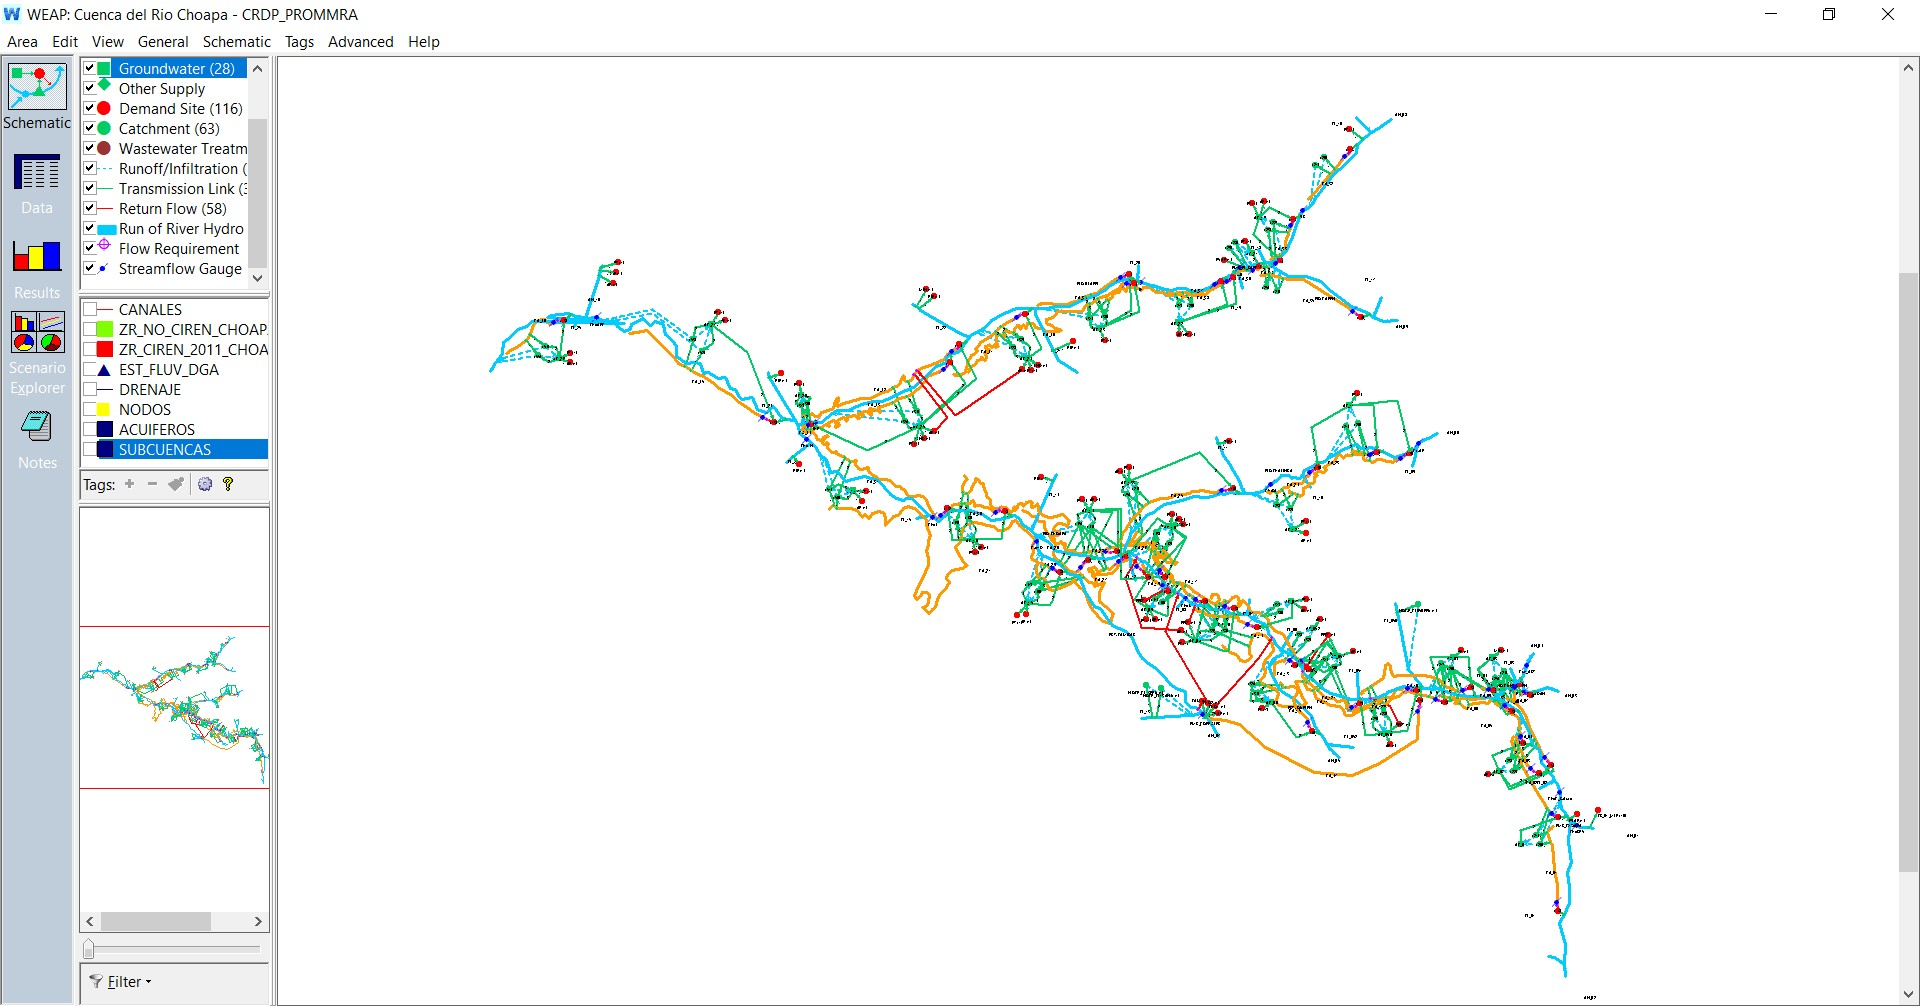
\includegraphics[width=\textwidth]{Logo/WEAPTopologia}}
\caption{Topología Modelo WEAP: Cuenca del río Choapa CRDP - PROMMRA}
\label{etiqueta_figura3}
\end{center}
\end{figure}

En el siguiente cuadro \ref{etiqueta_cuadro1} , se presenta la configuración topológica inicial del modelo Cuenca del río Choapa para sus distintos canales y, la fuente de cada uno de ellos. Además de los nombres de los canales, correspondiente a su respectiva agrupación. 

\begin{longtable}[c]{|l|l|l|}
\caption{Nomenclatura y composición de las agrupaciones de canales del modelo.}
\label{etiqueta_cuadro1}\\
\hline
\multicolumn{1}{|c|}{\textbf{\begin{tabular}[c]{@{}c@{}}Nomenclatura \\ WEAP\end{tabular}}} & \multicolumn{1}{c|}{\textbf{Nombre}} & \multicolumn{1}{c|}{\textbf{Fuente}} \\ \hline
\endfirsthead
%
\endhead
%
CA-01 & \begin{tabular}[c]{@{}l@{}}Los Morros, Cabecita de León, Eusebio,\\ Huinganal, Los Blancos, El Valle\end{tabular} & Río Valle \\ \hline
CA-02 & Piedrino & Río Choapa \\ \hline
CA-03 & Batuco, Manzano Derecho, Manzano Izquierdo & Río Choapa \\ \hline
CA-04 & Rodadero o Manzano & Río Choapa \\ \hline
CA-05 & Pangue o Inquilinos & Río Choapa \\ \hline
CA-06 & Molino de Tranquilla & Río Choapa \\ \hline
CA-07 & \begin{tabular}[c]{@{}l@{}}Molino de Tencadán, Tencadán Derecho,\\ Tencadán Izquierdo, Codicia o Las Pampitas, \\ Tencadán Cortadera Derecho, \\ Tencadán Aletón Izquierdo\end{tabular} & Río Tencadan \\ \hline
CA-08 & \begin{tabular}[c]{@{}l@{}}Buitrón, El Bosque, Los Loros o Los\\ Arriendos\end{tabular} & Río Cuncumén \\ \hline
CA-09 & Tiralarga & Río Cuncumén \\ \hline
CA-10 & Araya, Barraco Grande, Los Ranchos Choapa & Río Choapa \\ \hline
CA-11 & Silvano & Río Choapa \\ \hline
CA-120 & Barraco Chico, Del Sauco & Río Choapa \\ \hline
CA-121 & Aguas Claras de Chillepín, El Pavo & Río Choapa \\ \hline
CA-13 & El Molino de Quelén & Río Choapa \\ \hline
CA-14 & Breas o Molino de Llimpo & Río Choapa \\ \hline
CA-15 & De La Higuera, Potrero El Buey, Maitén & Est. Quelén \\ \hline
CA-16 & Panguecillo Uno o Del Medio, Panguecillo Dos & Río Choapa \\ \hline
CA-17 & Higueral & Río Choapa \\ \hline
CA-18 & Pardo & Río Choapa \\ \hline
CA-19 & El Queñe, Aguas Claras & Río Choapa \\ \hline
CA-20 & Población & Río Choapa \\ \hline
CA-21 & Buzeta & Río Choapa \\ \hline
CA-22 & Molino de Zapallar & Río Chalinga \\ \hline
CA-23 & Batuco de Chalinga & Río Chalinga \\ \hline
CA-24 & \begin{tabular}[c]{@{}l@{}}Alameda, Maravillal o La Viña, Palquial o\\ Molino de San Agustín, Valentino y Canelo\end{tabular} & Río Chalinga \\ \hline
CA-25 & \begin{tabular}[c]{@{}l@{}}Vert. Los Guindos, Vert. San Francisco,\\ Vert. Las Casas, Chañar Chalinga, Cunlagua, Huanque, \\ Arboleda Grande, Chalinga o Cancha Brava, \\ Chilcas, Tebal\end{tabular} & Río Chalinga \\ \hline
CA-26 & Tahuincano, Las Viudas & Río Choapa \\ \hline
CA-27 & Caracha & Río Choapa \\ \hline
CA-28 & El Boldo o Chuchiñí & Río Choapa \\ \hline
CA-29 & Jote, Camisas o Batito & Est. Camisas \\ \hline
CA-30 & \begin{tabular}[c]{@{}l@{}}El Molino de Peralillo, Las Chacras, Los\\ Loros o Del Medio\end{tabular} & Río Choapa \\ \hline
CA-31 & Pintacura Norte, Pintacura Sur o Alto & Río Choapa \\ \hline
CA-32 & \begin{tabular}[c]{@{}l@{}}Los Gonzalez, Salinas, Las Burras Bajas, El\\ Durazno Illapel, Los Perales Illapel, Las Burras Altas\end{tabular} & Río Illapel \\ \hline
CA-33 & \begin{tabular}[c]{@{}l@{}}Llano Alto, Llano Bajo, Covachas, Los Manque, \\ Alcantarilla, Pichicaven, Calderón,Mala Ladera, \\ El Agüita, Los Sauces, La Montaña,Rodado, \\ El Bajo, El Macal Illapel\end{tabular} & Río Illapel \\ \hline
CA-34 & Santa Margot & Río Illapel \\ \hline
CA-35 & \begin{tabular}[c]{@{}l@{}}Molino de Carén Illapel, Santa Ana, San\\ Arturo, Carrizo Carén, San Isidro Carén, \\ El Buitre Carén, Tizón\end{tabular} & Río Caren \\ \hline
CA-36 & Santa Margarita, El Palqui Illapel & Río Illapel \\ \hline
CA-37 & El Peumo, San Jorge, Santa Isabel, San Javier & Río Illapel \\ \hline
CA-38 & La Turbina & Río Illapel \\ \hline
CA-39 & \begin{tabular}[c]{@{}l@{}}Santa Olga, Los Pelados, San Isidro, El\\ Silo, San Patricio, Camarote, Escorial Illapel, \\ Plantación\end{tabular} & Río Illapel \\ \hline
CA-40 & La Higuera, Cocinera & Río Illapel \\ \hline
CA-41 & \begin{tabular}[c]{@{}l@{}}Vert. Luna, Hospital, Molino de Cárcamo,\\   Potrero Nuevo\end{tabular} & Río Illapel \\ \hline
CA-42 & \begin{tabular}[c]{@{}l@{}}Zepedino, Cuz Cuz, Población Los Guindos,\\   San Juan de Dios\end{tabular} & Río Illapel \\ \hline
CA-43 & \begin{tabular}[c]{@{}l@{}}Inquilinos o Del Bajo, Molino El Peral,\\   Bellavista o Del Alto, Del Medio o Bellavista Bajo\end{tabular} & Río Illapel \\ \hline
CA-44 & Junta El Maitén & Río Illapel \\ \hline
CA-45 & \begin{tabular}[c]{@{}l@{}}Coyuntagua Norte, Coyuntagua Sur Uno,\\ Coyuntagua Sur Dos, San Francisco, San Pedro,\\ Doña Juana, Mincha Norte,\\ Mincha Sur Arriba, Mincha Sur Abajo, \\ Matriz de Mincha, Tunga Norte Bajo\end{tabular} & Río Choapa \\ \hline
CA-46 & \begin{tabular}[c]{@{}l@{}}Salinero, Millahue Uno o Lílenes, Millahue\\ Dos o Los Patos, Los Rulos, San Antonio, \\ Molino de Choapa\end{tabular} & Río Choapa \\ \hline
CA-47 & Canal Alimentador Corrales & Río Choapa \\ \hline
\end{longtable}

\item \textbf{ \textit{Actualización de las acciones y capacidad de porteo}:} En el modelo WEAP de la cuenca del río Choapa, existe una sección llamada datos, en ella, podemos observar todos los \textit{inputs} que componen los nodos del modelo: \textit{Key Assumptions}, \textit{Demand Sites and Catchments}, \textit{Hydrology, Supply and Resources}, y \textit{Other Assumptions} (Figura \ref{etiqueta_figura4}).

\begin{figure}[H]
\begin{center}
\fbox{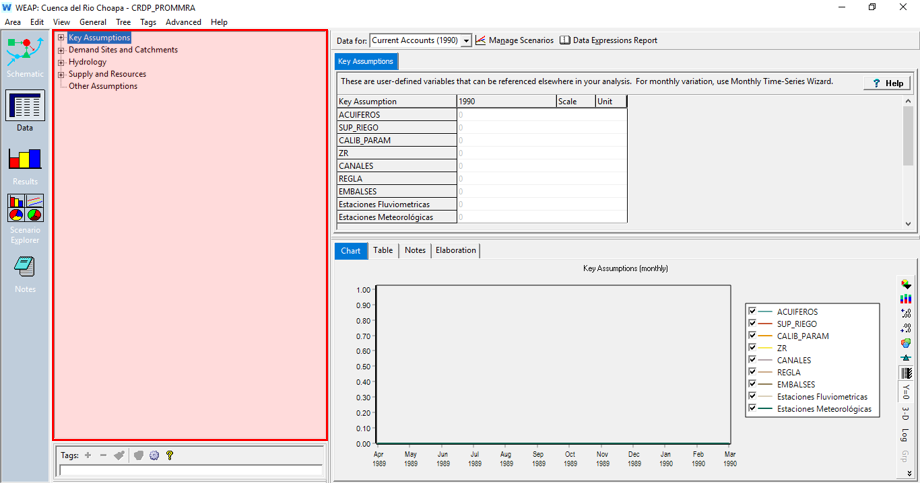
\includegraphics[width=\textwidth]{Logo/WEAP1}}
\caption{Herramientas del Modelo WEAP.}
\label{etiqueta_figura4}
\end{center}
\end{figure}


En la sección Key Assumptions, se especifican los datos que forman parte de la demanda u oferta del sistema, o datos matemáticos dentro del modelo, que permiten establecer algoritmos de cálculo o lógica. En esta sección, existen variables que permiten ir actualizando al modelo de acuerdo a la disponibilidad de datos y a la configuración establecida. En la sección CANALES, se observa que posee las variables ACCIONES, CAPACIDADES y PERDIDAS para las 3 organizaciones de la cuenca respectivamente (Figura \ref{etiqueta_figura5}).

\begin{figure}[H]
\begin{center}
\fbox{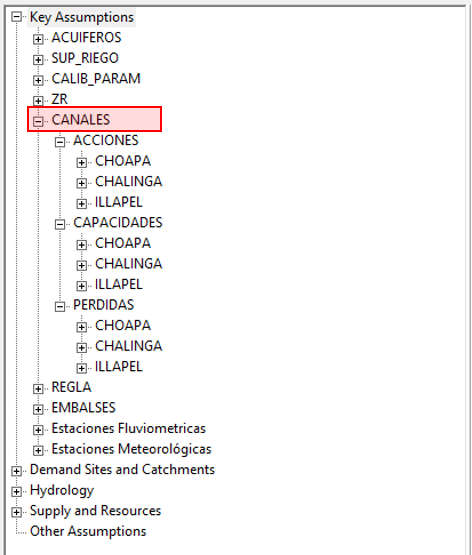
\includegraphics[width=\textwidth]{Logo/WEAP2}}
\caption{\textit{Key Assumptions del modelo}.}
\label{etiqueta_figura5}
\end{center}
\end{figure}





En la sección \textbf{ACCIONES}, es posible configurar el número de los derechos nominales que cada comunidad presenta de las tres Juntas de Vigilancia, en función de los litros/segundo que poseen sobre el río.

De igual manera, es posible configurar la capacidad de porteo ($L/s$) que cada canal posee, de acuerdo a cada organización. Esta variable se actualiza en la sección \textbf{CAPACIDADES}.

\item \textbf{\textit{Generación de escenarios de revestimiento}:} Para la generación de escenarios de revestimiento de canales, se procederá mejorando la eficiencia de conducción por cada agrupación, comparando los efectos frente al escenario base y, además a los grupos de canales dentro de su misma área de influencia de cada Junta de Vigilancia.

Para crear estos escenarios, se debe ingresar a la sección \textit{Data} del modelo y luego a \textit{Manage Scenarios}, tal como se observa en la figura \ref{etiqueta_figura6}.

\begin{figure}[H]
\begin{center}
\fbox{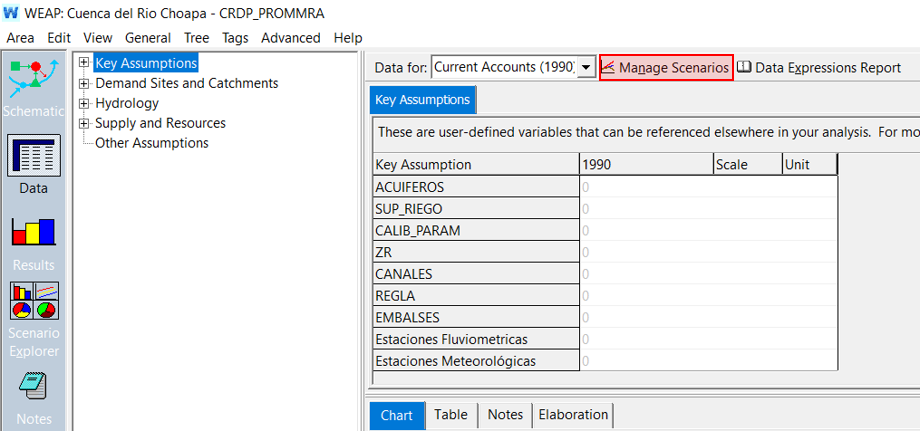
\includegraphics[width=\textwidth]{Logo/WEAP3}}
\caption{\textit{Manage Scenarios}.}
\label{etiqueta_figura6}
\end{center}
\end{figure}

En esta sección se crean los escenarios, en función de los cambios que se deseen realizar. En este caso, se desarrollan escenarios de mejoramiento en la eficiencia de conducción de los canales, basados en la conformación por grupos en el modelo. Se configurará como pérdida por conducción, de 0\%; esto representará el revestimiento de los canales en su totalidad.

Para ello, a partir del escenario base, se crea un nuevo escenario correspondiente al revestimiento de canales. En la pantalla Data, se creará automáticamente el escenario para su posterior configuración, (Figura \ref{etiqueta_figura7}).

En dicha pantalla y, en la sección de \textit{Key Assumptions}, se modifica en \textbf{PERDIDAS}, los valores del \% de pérdidas de los canales a revestir en el escenario. Posterior a ello se “corre” el modelo en la sección \textit{Results}, para la visualización de resultados de los distintos parámetros a evaluar. 

\begin{figure}[H]
\begin{center}
\fbox{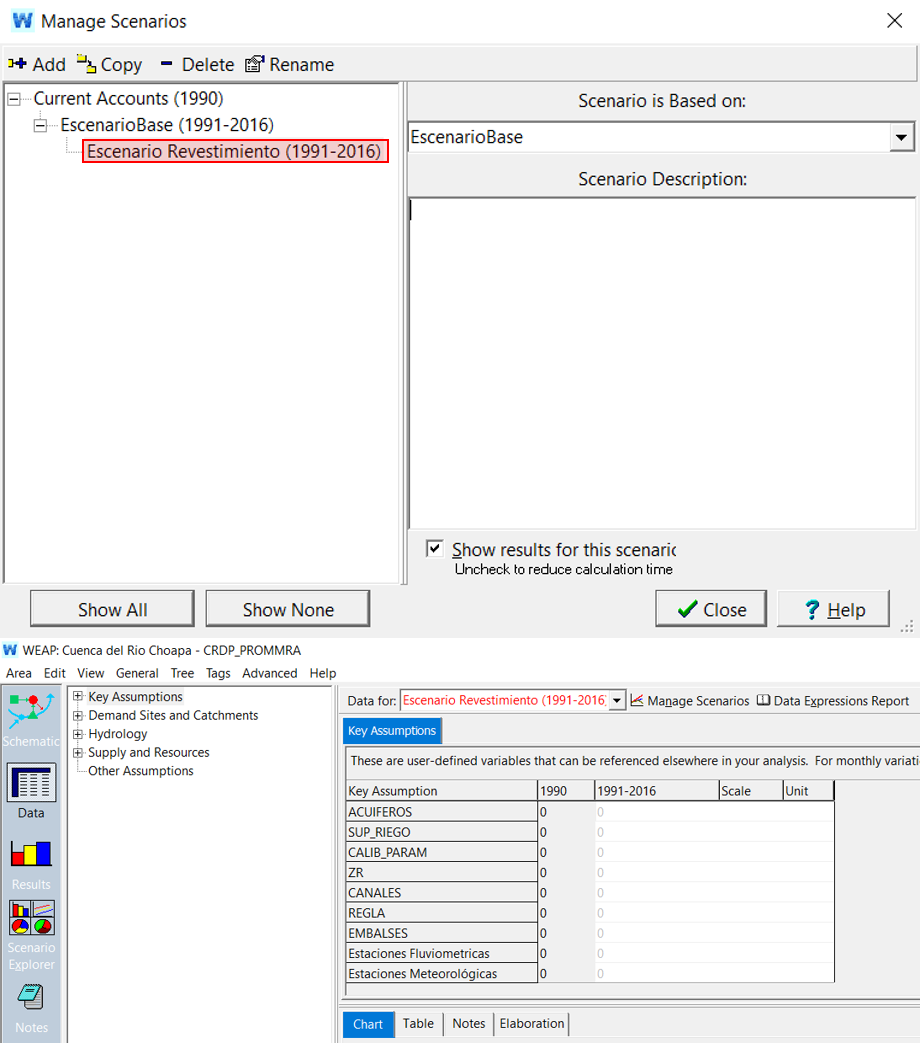
\includegraphics[width=\textwidth]{Logo/WEAP4}}
\caption{Creación de un nuevo escenario.}
\label{etiqueta_figura7}
\end{center}
\end{figure}

Cada parámetro a evaluar, se analiza en el campo de los resultados, configurando la visualización de la manera más óptima para su comprensión. Es decir, WEAP permite ajustar la visualización en función de la serie temporal, unidades de medida, tipos de gráficos, parámetros a comparar, entre otros. Cada resultado se puede descargar en formato \textit{.XLSX} o \textit{.CSV} para su análisis externo.\\
\\
El resultado de la modelación hidrológica nos permitirá establecer que agrupación de canales genera beneficios o efectos negativos sobre una zona en particular de la cuenca.

\end{itemize}

\subsection{Componente 1. Actividad 1.4. Validación del protocolo técnico-social de inversión en mejoramiento de la eficiencia de conducción hídrica.}

Se seleccionaron tres Comunidades de aguas, denominadas Chalinga o Cancha Brava, Arboleda Grande y Huanque, las que se encuentran bajo la jurisdicción de la Junta de Vigilancia del Río Chalinga y sus Afluentes, en la cuenca del río Chalinga. Se enfocará en esta cuenca con el fin de avanzar en la creación del primer Plan de priorización para la OUA's comprometido.

\subsubsection{Recopilación de información.}

\begin{itemize}
	\item[$-$] \textbf{Recopilación bibliográfica cuenca río Chalinga}
\end{itemize}

Como primera información, se recopiló la ficha de registros de bocatomas, generada por la Dirección General de Aguas, junto con la información geoespacial denominada Canales de riego a nivel matrices hasta 2do derivado de la Comisión Nacional de Riego. Además estos antecedentes no permitirán apoyarnos en el levantamiento del S.I.G. y determinación de superficies bajo riego y superficie potencial.

\begin{itemize}
	\item[$-$] \textbf{Información Junta de Vigilancia Río Chalinga y sus Afluentes}
\end{itemize}

A través de mesas de trabajo conformadas por el equipo del proyecto y la organización, se recopiló la siguiente información:

\begin{itemize}	
	\item Diagrama unifilar: Recopilación de archivos en formato pdf.
	\item Ubicación geográfica bocatomas: Apoyo para ubicación de bocatomas con el Sr. Wenceslao Layana, Asesor Técnico.
	\item Número de acciones totales: Revisión de archivos, recopilado mediante digitalización.
	\item Número de acciones por comunidad de aguas: Revisión de archivos, recopilado mediante digitalización.
	\item Dotaciones o desmarques: Revisión de archivos, recopilado mediante digitalización.
	\item Capacidad de porteo de cada canal: Información no disponible, se estableció un 10\% extra de la entrega total en $l/s$.
	\item Número de usuarios comunidad de aguas: Recopilación de archivos actualizados por el programa de fortalecimiento de la CNR en ejecución en la organización.
	\item Superficie regada por comunidad de aguas: Revisión de archivos, recopilado mediante digitalización.
	\item Contacto celadores: Se realiza en forma constante con el Sr. Wenceslao Layana, Asesor Técnico de la OUA's.
\end{itemize}
\clearpage
\begin{itemize}
	\item[$-$] \textbf{Información Comunidad de Aguas Chalinga o Cancha Brava}
\end{itemize}

Se realizó la entrevista a un representante de la Comunidad de aguas, los antecedentes recolectados se presentan a continuación:

\begin{figure} [H]
	\fbox{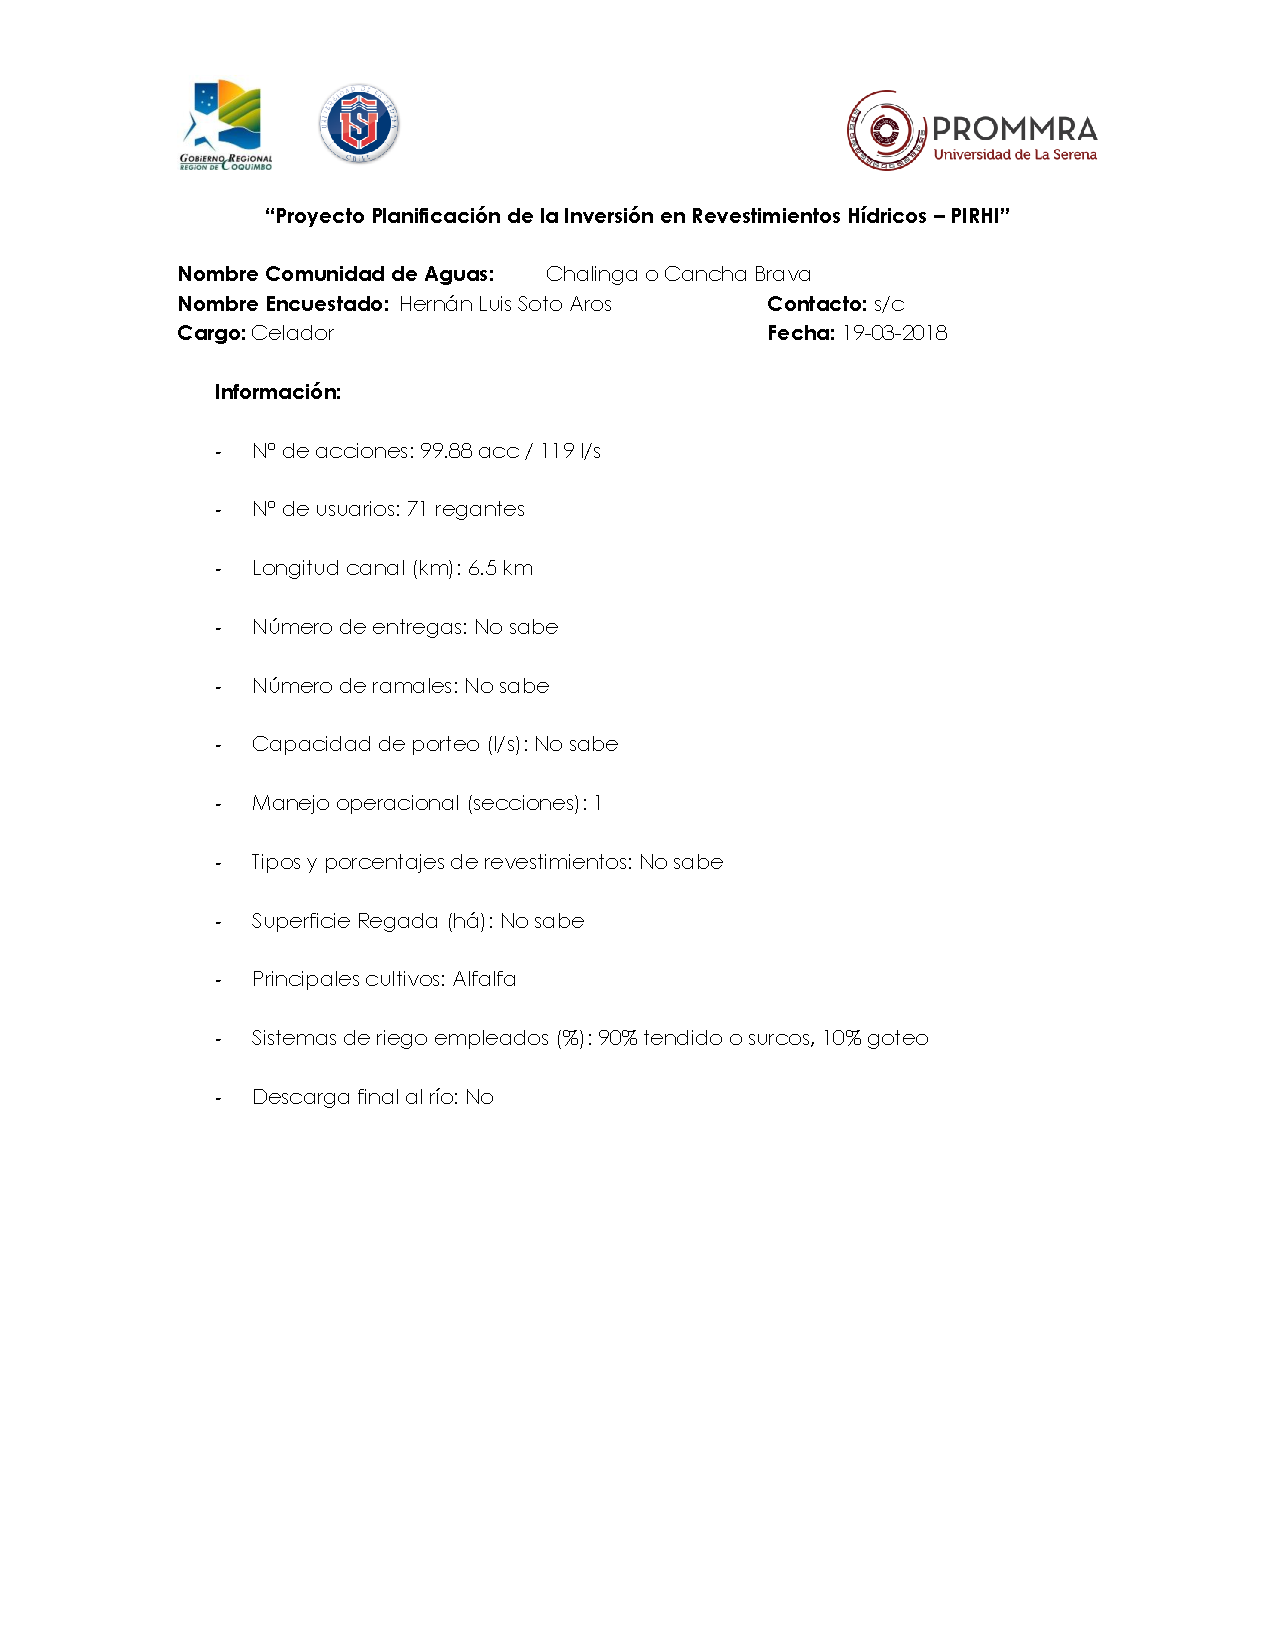
\includegraphics[height=19cm]{EntrevistasCA/Chalinga.pdf}}
	\caption{Entrevista Comunidad de aguas Chalinga o Cancha Brava.}
\end{figure}
\clearpage
\begin{itemize}
	\item[$-$] \textbf{Información Comunidad de Aguas Arboleda Grande}
\end{itemize}

Se realizó la entrevista a un representante de la Comunidad de aguas, los antecedentes recolectados se presentan a continuación:

\begin{figure} [H]
  \fbox{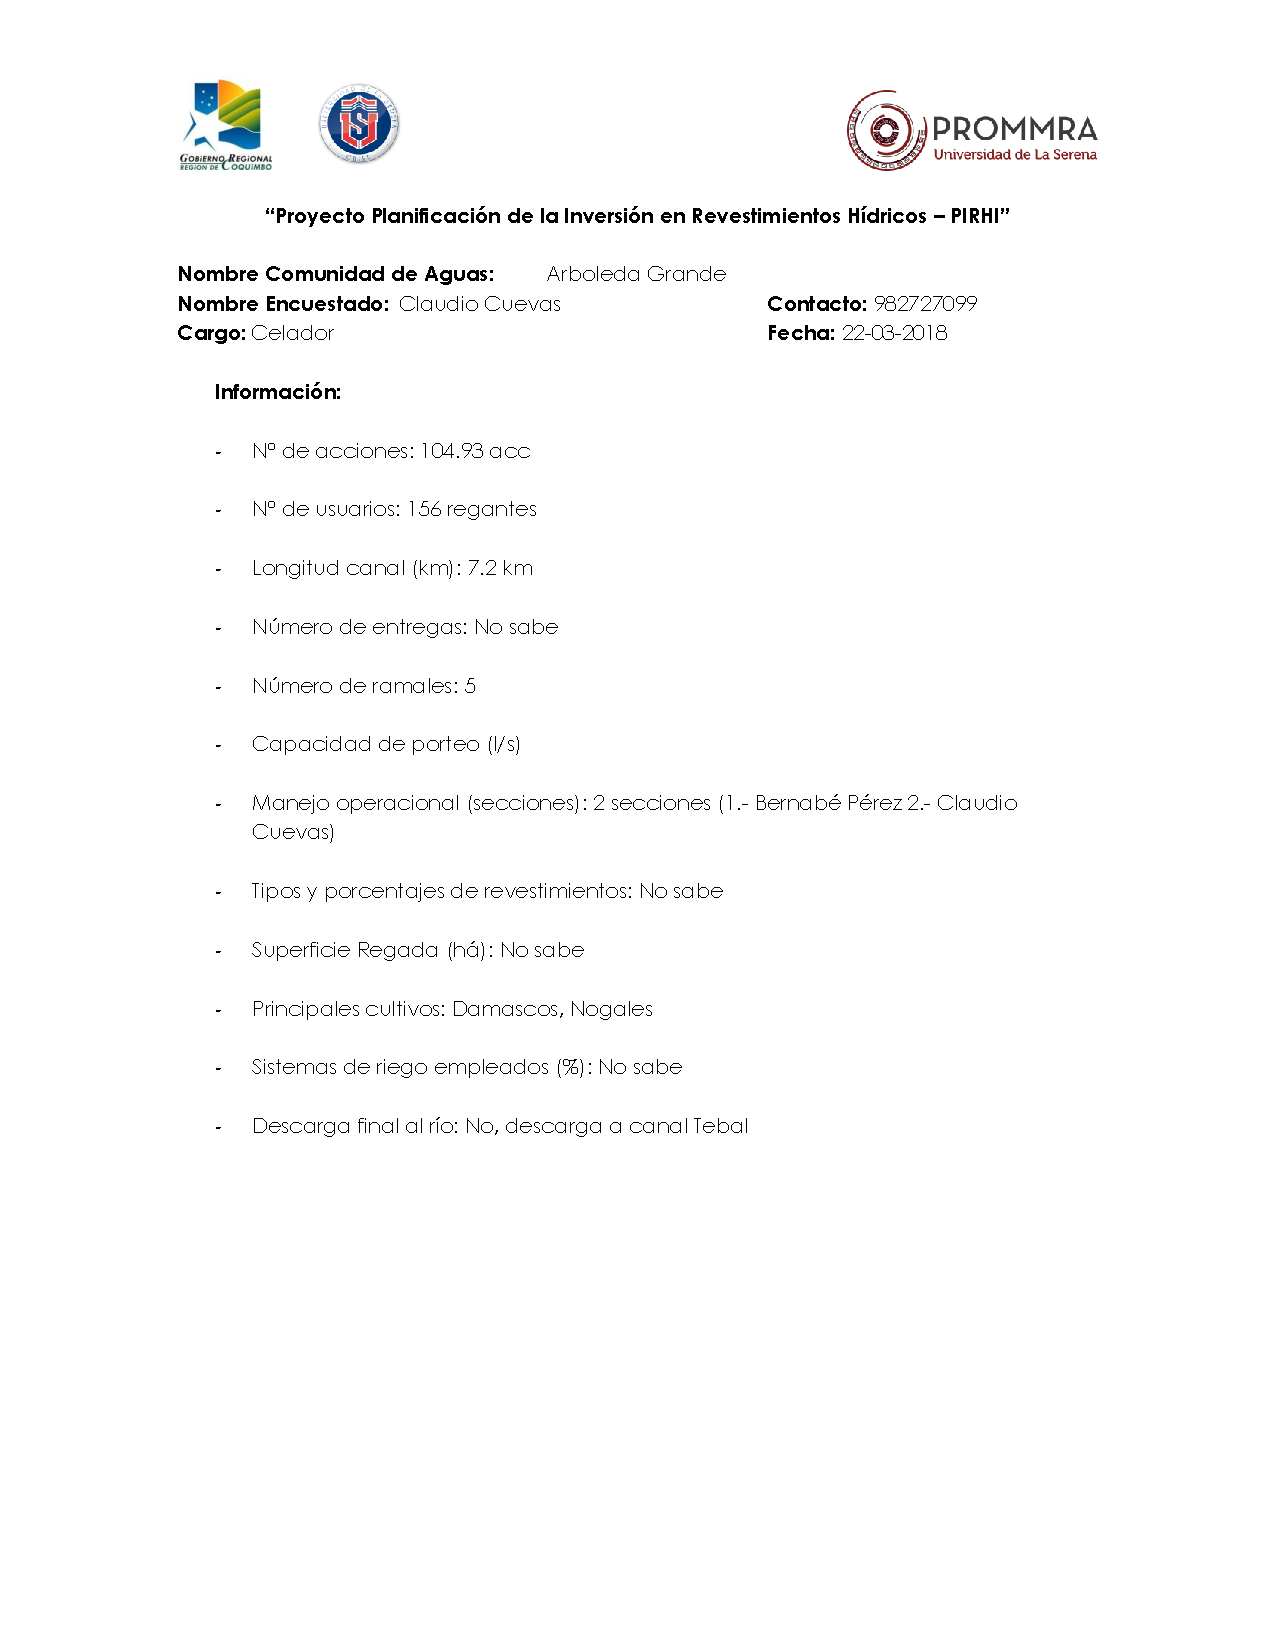
\includegraphics[height=19cm]{EntrevistasCA/Arboleda_grande.pdf}}
	\caption{Entrevista Comunidad de aguas Arboleda grande.}
\end{figure}
\clearpage
\begin{itemize}
	\item[$-$] \textbf{Información Comunidad de Aguas Huanque}
\end{itemize}

Se realizó la entrevista a un representante de la Comunidad de aguas, los antecedentes recolectados se presentan a continuación:

\begin{figure} [H]
  \fbox{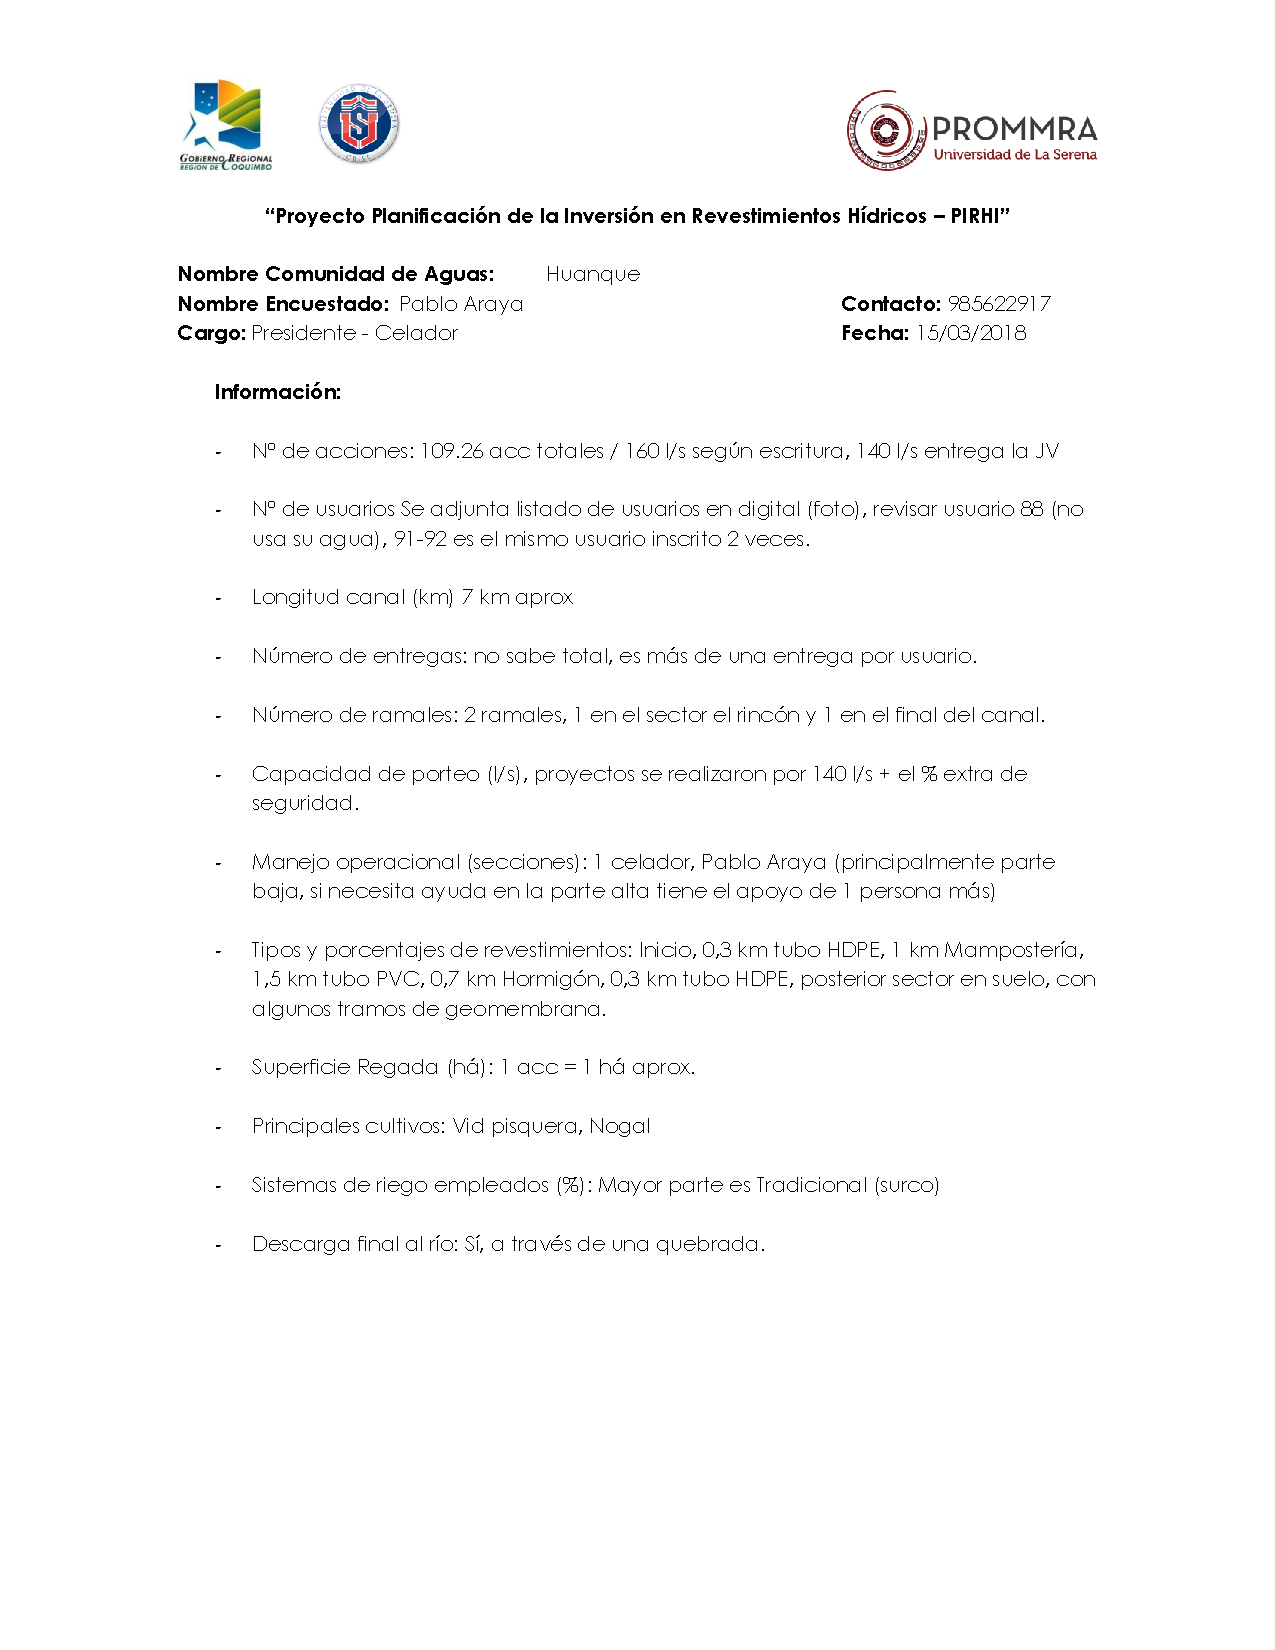
\includegraphics[height=19cm]{EntrevistasCA/Huanque.pdf}}
	\caption{Entrevista Comunidad de aguas Huanque.}
\end{figure}
\clearpage
Como resultado de la recopilación de información a nivel de cuenca, OUA's y Comunidades de aguas, se pudo obtener la siguientes información:

\begin{table}[H]
\caption{Variables obtenidas de la recopilación de Información}
\begin{tabular}{l|c|c|c|}
\cline{2-4}
  & \multicolumn{3}{c|}{\textbf{Comunidades de Aguas o canal}                                                          } \\ \hline
\multicolumn{1}{|c|}{\textbf{\begin{tabular}[c]{@{}c@{}}Variable \\\end{tabular}}} & \textbf{Arboleda Grande} & \textbf{Chalinga o Cancha Brava} & \textbf{Huanque}         \\ \hline
\multicolumn{1}{|l|}{\textbf{Número de acciones}}       & 98,78 & 104,93 & 109,26\\
\multicolumn{1}{|l|}{\textbf{Capacidad de porteo ($l/s$)}}        &   129,9   &     165     &  154 \\
\multicolumn{1}{|l|}{\textbf{Número de beneficiarios}}        & 85 & 160 & 97\\ \hline
\end{tabular}
\end{table}

\subsubsection{Sistema de Información Geográfica (S.I.G.).}

En una primera campaña de terreno, realizada en el mes de Marzo, se realizaron por completo la georeferenciación de 3 canales correspondiente al área de la Junta de Vigilancia del Río Chalinga y sus Afluentes. Se llevo a cabo en 3 canales de la segunda sección del río Chalinga, la cual posee la mayor longitud en la red de canales con 41,62 km (según capa canales CNR), por la operatividad y disponibilidad de personal de las comunidades de agua que conforman el área de Chalinga, las comunidades de aguas Arboleda Grande, Chalinga o Cancha Brava y Huanque, representan el 12,5\%, 8,8\% y 16,7\% de la longitud total de la red de la segunda sección del río respectivamente según los datos obtenidos de CNR.\\
\\
Mediante GPS diferencial y el diccionario incorporado a estos, se logró georeferenciar y describir cada uno de las obras a levantar en el recorrido de los canales. A modo de resumen se presenta la información recabada en las bocatoma de estos canales.

\begin{table}[H]
\caption{Descripción Bocatomas}
\label{my-label}
\begin{tabular}{l|c|c|c|}
\cline{2-4}
                                                                                              & \multicolumn{3}{c|}{\textbf{Canales}                                                          } \\ \hline
\multicolumn{1}{|c|}{\textbf{\begin{tabular}[c]{@{}c@{}}Componente \\ Bocatoma\end{tabular}}} & \textbf{Arboleda Grande} & \textbf{Chalinga o Cancha Brava} & \textbf{Huanque}         \\ \hline
\multicolumn{1}{|l|}{\textbf{Obra desviación}}                                               & Barrera lateral          & Compuerta hoja metálica          & Barrera lateral          \\
\multicolumn{1}{|l|}{\textbf{Canal aducción}}                                                 & 867,45 m                 & 568,18 m                         & 184,73 m                 \\
\multicolumn{1}{|l|}{\textbf{Compuerta Carga}}                                                & Compuerta manual & Compuerta manual         & Compuerta manual \\
\multicolumn{1}{|l|}{\textbf{Sección Control}}                                                & Aforador Parshall        & Aforador Parshall                & Aforador Parshall        \\ \hline
\end{tabular}
\end{table}

La caracterización realizada a nivel de canal presenta información como longitud y tipos de revestimientos, estructuras de distribución y puntos críticos. Además esta información nos permitirá definir los tramos para evaluación de pérdidas por conducción, proporcionar las dimensiones de la sección afecta a revestimiento, validar o ajustar el trazado del canal que en primera instancia se obtuvo de la capa de la CNR, y así rectificar las superficies asociadas a cada canal, las cuales fueron asignadas en base la capa CNR.\\
\\ 
Para la definición de la longitud que utiliza el protocolo, se recolectó las coordenadas, revestimiento (número de paredes del canal revestida), tipo de revestimiento (permanente o temporal) y material de revestimiento en cada cambio de revestimiento, lo que permite dar cumplimiento para la definición de estas longitudes.\\
\\
A continuación se presenta un resumen de longitudes que presentan los 3 canales validados.

\begin{table}[H]
\centering
\caption{Longitudes por canal}
\label{my-label}
\resizebox{\textwidth}{!}{%
\begin{tabular}{|l|c|c|c|}
\hline
\textbf{Canal}           & \textbf{Canal aducción ($km$)} & \textbf{Canal conducción y distribución ($km$)} & \textbf{Total General ($km$)} \\ \hline
\textbf{Arboleda Grande} & 0,87  & 5,03 & 5,90   \\ \hline
\textbf{Cancha Brava}    & 0,57  & 3,84 & 4,41 \\ \hline
\textbf{Huanque}        & 0,18  & 7,01   & 7,19 \\ \hline
\end{tabular}%
}
\end{table}

Para las estructuras de distribución mediante la captura de sus coordenadas y caracterización del tipo de obra, se obtiene el requerimiento que permitirá definir tramo matriz y puntos de entrega tomándose en cuenta para la evaluación de pérdidas. \\
\\
En la validación se obtiene que los canales presentan los siguientes estructuras de distribución.

\begin{table}[H]
\centering
\caption{Estructuras de distribución}
\label{my-label}
\begin{tabular}{l|c|c|c|c}
\cline{2-4}
                                                       & \multicolumn{3}{c|}{\textbf{Estructura distribución}} & \multicolumn{1}{l}{}                        \\ \hline
\multicolumn{1}{|l|}{\textbf{Canal}}                   & \textbf{Entrega}  & \textbf{Gestión} & \textbf{Ramal} & \multicolumn{1}{c|}{\textbf{Total general}} \\ \hline
\multicolumn{1}{|l|}{\textbf{Arboleda Grande}}         & 88                & 32               & 7              & \multicolumn{1}{c|}{127}                    \\ \hline
\multicolumn{1}{|l|}{\textbf{Chalinga o Cancha Brava}} & 68                & 53               & 5              & \multicolumn{1}{c|}{126}                    \\ \hline
\multicolumn{1}{|l|}{\textbf{Huanque}}                 & 100               & 56               & 3              & \multicolumn{1}{c|}{159}                    \\ \hline
\end{tabular}
\end{table}

Dentro de las estructuras de distribución se agrega la función de ramal, la cual no se consideraba para el protocolo del proyecto SIMCA-Elqui, esta función busca conocer donde nacen los derivados y estimar superficie irrigada por el ramal, ajustando la asignación de la superficie a los canales si se encuentra más de un canal cercano en el territorio.\\
\\
En el recorrido de canal se obtuvieron coordenadas de inicio, fin y algunos puntos críticos que se presenten en el canal, como filtraciones, quebradas, desbordes, entre otros, que puedan afectar la conducción y distribución normal del recurso, por lo cual dependiendo del tipo de observación y longitud de este hito se definirá si es necesario realizar un subtramo adicional para evaluación de pérdidas los cuales son definidos por los cambios de revestimientos.\\
\\
Los resultados obtenidos para la validación de variables que contemple el protocolo como insumos para priorización con se presentan a continuación: 

% Please add the following required packages to your document preamble:
% \usepackage{graphicx}
\begin{table}[H]
\caption{Resultados variables longitudes y dimensiones}
\begin{tabular}{|l|ccc|}
\hline
\textbf{Variables}  & \textbf{Arboleda Grande} & \textbf{Chalinga o} & \textbf{Huanque} \\
 & & \textbf{Cancha Brava} &  \\ \hline                          
\textbf{Longitud total de canal en uso ($km$)}   & 5.902    & 4.406    & 7.190  \\
\textbf{Longitud tramo matriz ($km$)}  & 0.046    & 0.045    & 0.071    \\
\textbf{Longitud Tramo conducción ($km$)}  & 4.989  & 3.792  & 6.934   \\
\textbf{Longitud afecta a mejoramiento ($km$)}   & 2.149     & 2.306   & 2.472  \\
\textbf{*Dimensiones a revestir  (ancho; alto) ($m$)} & 0,6; 0,5 & 0,9; 0,7 & 0,5; 0,4\\ 
\hline
\end{tabular}
\small{*Sección rectangular revestida en hormigón}\\
\end{table}

\subsubsection{Determinación general de pérdidas.}

La información del S.I.G. nos permite generar los tramos de aforo para la determinación de pérdidas, basado en la primera entrega para definir el tramo matriz (se presentan los datos en color rojo) y tipos de revestimientos presentes. A continuación se presentan los tramos generados para cada Comunidad de aguas.

\begin{itemize}
	\item[$-$] \textbf{Comunidad de Aguas Chalinga o Cancha Brava}
\end{itemize}

\begin{table}[H]
\centering
\caption{Tramos del canal Chalinga o Cancha Brava.}
\label{matriz}
\begin{tabular}{|c|c|c|c|c|c|c|c|}
\hline
\textbf{Tramo} & \textbf{\begin{tabular}[c]{@{}c@{}}N°\\ aforo \\ inicial\end{tabular}} & \textbf{\begin{tabular}[c]{@{}c@{}}N°\\ aforo\\ final\end{tabular}} & \textbf{\begin{tabular}[c]{@{}c@{}}Km\\ inicial\end{tabular}} & \textbf{\begin{tabular}[c]{@{}c@{}}Km\\ final\end{tabular}} & \textbf{\begin{tabular}[c]{@{}c@{}}Longitud\\ ($km$)\end{tabular}} & \textbf{Revestimiento}   & \textbf{Hitos} \\ \hline                                                                                   
{\color[HTML]{FE0000} \textbf{1}} & {\color[HTML]{FE0000} \textbf{1}} & {\color[HTML]{FE0000} \textbf{2}} & {\color[HTML]{FE0000} \textbf{0,00}}& {\color[HTML]{FE0000} \textbf{0,04}} & {\color[HTML]{FE0000} \textbf{0,04}} & {\color[HTML]{FE0000} \textbf{Hormigón}} & {\color[HTML]{FE0000} \textbf{Sección Matriz}} \\ \hline
\textbf{2} & 2 & 20 & 0,04 & 1,37 & 1,33 & Hormigón & - \\ \hline
\textbf{3} & 20 & 23 & 1,37 & 1,70 & 0,33 & Geomembrana & - \\ \hline
\textbf{4} & 23 & 26 & 1,70 & 1,80 & 0,10 & \begin{tabular}[c]{@{}c@{}}Hormigón - \\ Loseta\end{tabular} & - \\ \hline                                                                                             
\textbf{5} & 26 & 73 & 1,80 & 3,84 & 2,04 & Geomembrana & - \\ \hline                                                                                      
\end{tabular}
\end{table}

El trazado del canal Chalinga o Cancha Brava se encuentra revestido en su totalidad, donde se presentan revestimientos de tipo permanente y temporal. Este se dividió en 5 tramos, los que se desglosan en el tramo matriz y 4 tramos de distribución. El tramo matriz o 1, junto a los tramos de distribución 2 y 4, presentan revestimientos de tipo permanente, cuyo material principal es hormigón. Los tramos 3 y 5, corresponde a geomembrana, la cual es de tipo temporal y poseen en conjunto una longitud de 2,37 $km$.

\begin{itemize}
	\item[$-$] \textbf{Comunidad de Aguas Arboleda Grande.}
\end{itemize}

\begin{table}[H]
\centering
\caption{Tramos del canal Arboleda Grande.}
\label{matriz}
\begin{tabular}{|c|c|c|c|c|c|c|c|}
\hline
\textbf{Tramo} & \textbf{\begin{tabular}[c]{@{}c@{}}N°\\ aforo \\ inicial\end{tabular}} & \textbf{\begin{tabular}[c]{@{}c@{}}N°\\ aforo\\ final\end{tabular}} & \textbf{\begin{tabular}[c]{@{}c@{}}Km\\ inicial\end{tabular}} & \textbf{\begin{tabular}[c]{@{}c@{}}Km\\ final\end{tabular}} & \textbf{\begin{tabular}[c]{@{}c@{}}Longitud\\ ($km$)\end{tabular}} & \textbf{Revestimiento}   & \textbf{Hitos} \\ \hline                                                                                   
{\color[HTML]{FE0000} \textbf{1}} & {\color[HTML]{FE0000} \textbf{1}} & {\color[HTML]{FE0000} \textbf{2}} & {\color[HTML]{FE0000} \textbf{0,00}}& {\color[HTML]{FE0000} \textbf{0,05}} & {\color[HTML]{FE0000} \textbf{0,05}} & {\color[HTML]{FE0000} \textbf{Mezcla suelo}} & {\color[HTML]{FE0000} \textbf{Sección Matriz}} \\ \hline
\textbf{2} & 2 & 7 & 0,05 & 0,34 & 0,29 & Mezcla suelo & - \\ \hline
\textbf{3} & 7 & 21 & 0,34 & 0,94 & 0,60 & Geomembrana & - \\ \hline
\textbf{4} & 21 & 45 & 0,94 & 2,18 & 1,24 & Loseta & - \\ \hline                                                                                             
\textbf{5} & 46 & 48 & 2,18 & 2,37 & 0,19 & \begin{tabular}[c]{@{}c@{}}Tubo PVC - \\ Tubo metálico\end{tabular} & - \\ \hline                                                                                      
\textbf{6} & 48 & 66 & 2,37 & 3,20 & 0,84 & Loseta & - \\ \hline
\textbf{7} & 66 & 79 & 3,20 & 3,77 & 0,57 & Hormigón & - \\ \hline                                                                                                                                                                            
\textbf{8} & 79 & 104 & 3,77 & 4,99 & 1,21 & Mezcla suelo & - \\ \hline                                                                                      
\textbf{9} & 104 & 105 & 4,99 & 5,03 & 0,05 & Tubo PVC & - \\ \hline                                                                                      
\end{tabular}
\end{table}

El trazado del canal se dividió en 9 tramos. La longitud total de los tramos a evaluar es de 5,03 $km$, de los cuales los primeros 0,6 $km$ corresponden a sin revestimiento o revestimiento temporal. Los siguientes 2,84 $km$, corresponden a revestimiento de tipo permanente, del cual se destaca el material de tipo loseta. La parte final del trazado se encuentra sin revestimiento en su mayoría, solo los últimos 0,05 $km$ se encuentran en tubo de PVC.
\clearpage
\begin{itemize}
	\item[$-$] \textbf{Comunidad de Aguas Huanque.}
\end{itemize}

\begin{table}[H]
\centering
\caption{Tramos del canal Huanque.}
\label{matriz}
\begin{tabular}{|c|c|c|c|c|c|c|c|}
\hline
\textbf{Tramo} & \textbf{\begin{tabular}[c]{@{}c@{}}N°\\ aforo \\ inicial\end{tabular}} & \textbf{\begin{tabular}[c]{@{}c@{}}N°\\ aforo\\ final\end{tabular}} & \textbf{\begin{tabular}[c]{@{}c@{}}Km\\ inicial\end{tabular}} & \textbf{\begin{tabular}[c]{@{}c@{}}Km\\ final\end{tabular}} & \textbf{\begin{tabular}[c]{@{}c@{}}Longitud\\ ($km$)\end{tabular}} & \textbf{Revestimiento}   & \textbf{Hitos} \\ \hline                                                                                   
{\color[HTML]{FE0000} \textbf{1}} & {\color[HTML]{FE0000} \textbf{1}} & {\color[HTML]{FE0000} \textbf{2}} & {\color[HTML]{FE0000} \textbf{0,00}}& {\color[HTML]{FE0000} \textbf{0,02}} & {\color[HTML]{FE0000} \textbf{0,02}} & {\color[HTML]{FE0000} \textbf{Hormigón Roca}} & {\color[HTML]{FE0000} \textbf{Sección Matriz}} \\ \hline
{\color[HTML]{FE0000} \textbf{2}} & {\color[HTML]{FE0000} \textbf{2}} & {\color[HTML]{FE0000} \textbf{3}} & {\color[HTML]{FE0000} \textbf{0,02}}& {\color[HTML]{FE0000} \textbf{0,07}} & {\color[HTML]{FE0000} \textbf{0,05}} & {\color[HTML]{FE0000} \textbf{Tubo HDPE}} & {\color[HTML]{FE0000} \textbf{\begin{tabular}[c]{@{}c@{}}Término sección\\ Matriz\end{tabular}}} \\ \hline
\textbf{3} & 3 & 5 & 0,07 & 0,46 & 0,39 & Tubo HDPE & - \\ \hline
\textbf{4} & 5 & 19 & 0,46 & 1,49 & 1,03 & Hormigón Roca & - \\ \hline                                                                                             
\textbf{5} & 19 & 52 & 1,49 & 3,40 & 1,91 & Tubo PVC & - \\ \hline                                                                                      
\textbf{6} & 52 & 56 & 3,40 & 4,04 & 4,53 & Hormigón & - \\ \hline
\textbf{7} & 56 & 64 & 4,04 & 4,53 & 0,50 & Tubo HDPE & - \\ \hline                                                                                                                                                                            
\textbf{8} & 64 & 71 & 4,53 & 4,76 & 0,22 & Mezcla suelo & - \\ \hline                                                                                      
\textbf{9} & 71 & 96 & 4,76 & 5,70 & 0,95 & Geomembrana & - \\ \hline                                                                                      
\textbf{10} & 96 & 110 & 5,70 & 6,14 & 0,44 & Mezcla suelo & - \\ \hline
\textbf{11} & 110& 113 & 6,14 & 6,83 & 0,68 & Geomembrana & - \\ \hline
\textbf{12} & 113 & 119 & 6,83 & 7,01 & 0,18 & Mezcla suelo & - \\ \hline
\end{tabular}
\end{table}

Para el canal Huanque se generó un total de 12 tramos, de los cuales los 2 primeros corresponden a canal matriz, debido al cambio de revestimiento presente. Hasta el 4,53 $km$ de recorrido se presentan revestimientos de tipo permanente, mientras que los 2,48 $km$ restantes no presentan revestimiento o corresponde a tipo temporal.

La campaña de aforos se desarrollo en el mes de Abril. Al realizar los aforos de inicio y fin de cada tramo, se procedió a realizar la evaluación de pérdidas para una posible subdivisión. Los resultados se presentan a continuación.

\clearpage
\begin{landscape}
\begin{itemize}
	\item[$-$] \textbf{Comunidad de Aguas Chalinga o Cancha Brava.}
\end{itemize}

\begin{table}[H]
\centering
\caption{Tramos aforados del canal Chalinga o Cancha Brava.}
\label{matriz}
\resizebox{23cm}{!} {
\begin{tabular}{|c|c|c|c|c|c|c|c|c|c|c|c|c|c|}
\hline
\textbf{Tramo} & \textbf{\begin{tabular}[c]{@{}c@{}}N°\\ aforo \\ inicial\end{tabular}} & \textbf{\begin{tabular}[c]{@{}c@{}}N°\\ aforo\\ final\end{tabular}} & \textbf{\begin{tabular}[c]{@{}c@{}}Km\\ inicial\end{tabular}} & \textbf{\begin{tabular}[c]{@{}c@{}}Km\\ final\end{tabular}} & \textbf{\begin{tabular}[c]{@{}c@{}}Longitud\\ ($km$)\end{tabular}} & \textbf{\begin{tabular}[c]{@{}c@{}}Q Inicial\\ ($l/s$)\end{tabular}}   & \textbf{\begin{tabular}[c]{@{}c@{}}Q Final\\ Real ($l/s$)\end{tabular}} & \textbf{\begin{tabular}[c]{@{}c@{}}Q Antes\\ Entrega o\\ Aporte ($l/s$)\end{tabular}} & \textbf{\begin{tabular}[c]{@{}c@{}}Q Después\\ Entrega o\\ Aporte ($l/s$)\end{tabular}} & \textbf{\begin{tabular}[c]{@{}c@{}}Q  Entrega o\\ Aporte ($l/s$)\end{tabular}} & \textbf{\begin{tabular}[c]{@{}c@{}}Q  Final\\ Teórico ($l/s$)\end{tabular}} & \textbf{\begin{tabular}[c]{@{}c@{}}Pérdidas\\ ($l/s$)\end{tabular}} & \textbf{\begin{tabular}[c]{@{}c@{}}Pérdidas\\ ($\%$)\end{tabular}} \\ \hline                                                                                   
{\color[HTML]{FE0000} \textbf{1}} & {\color[HTML]{FE0000} \textbf{1}} & {\color[HTML]{FE0000} \textbf{2}} & {\color[HTML]{FE0000} \textbf{0,00}}& {\color[HTML]{FE0000} \textbf{0,04}} & {\color[HTML]{FE0000} \textbf{0,04}} & {\color[HTML]{FE0000} \textbf{54,07}} & {\color[HTML]{FE0000} \textbf{54,07}} & & & & {\color[HTML]{FE0000} \textbf{54,07}} & {\color[HTML]{FE0000} \textbf{0,00}} & {\color[HTML]{FE0000} \textbf{0,00}} \\ \hline
\textbf{2} & 2 & 20 & 0,04 & 1,37 & 1,33 & 54,07 & 51,30 & & & & 51,30 & 2,77 & 5,12 \\ \hline
\textbf{3} & 20 & 23 & 1,37 & 1,70 & 0,33 & 51,30 & 35,35 & & & & 35,35 & 15,95 & 31,09 \\ \hline
\textbf{4} & 23 & 26 & 1,70 & 1,80 & 0,10 & 35,35 & 35,35 & & & & 35,35 & 0,00 & 0,00 \\ \hline                                                                                             
\textbf{5.1} & 26 & 46 & 1,80 & 2,89 & 1,09 & 35,35 & 34,22 & & & & 34,22 & 1,13 & 3,20 \\ \hline                                                                                      
\textbf{5.2} & 46 & 73 & 2,89 & 3,84 & 0,94 & 34,22 & 22,41 & & & & 22,41 & 11,81 & 34,51 \\ \hline                                                                                      
\end{tabular}
}
\end{table}

La determinación de pérdidas por tramos del canal Chalinga o Cancha Brava, muestra que la mayor pérdida por conducción se produce en los tramos 3 y 5, en donde este último generó 2 subtramos debido a su alta pérdida. El tramo 3 presenta un 31,09$\%$ de pérdidas, donde se puedo apreciar el mal estado de la geomembrana presente y una alta concentración de vegetación. El subtramo 5.2, correspondiente al trazado final del canal, presenta una pérdida del 34,51$\%$, con un revestimiento de tipo temporal, convirtiéndose en el sector con mayores pérdidas, lo que puede deberse a la mala instalación de la geomembrana en algunos sectores. Los tramos restantes presentan pérdidas menores al 6$\%$. 

\begin{table}[H]
\centering
\caption{Pérdidas generales del canal Chalinga o Cancha Brava.}
\label{matriz}
\resizebox{23cm}{!} {
\begin{tabular}{|c|c|c|c|c|c|c|c|c|c|c|}
\hline
\textbf{Tramo} & \textbf{\begin{tabular}[c]{@{}c@{}}Q Inicial\\ ($l/s$)\end{tabular}}   & \textbf{\begin{tabular}[c]{@{}c@{}}Q Final\\ Real ($l/s$)\end{tabular}} & \textbf{\begin{tabular}[c]{@{}c@{}}Q Antes\\ Entrega o\\ Aporte ($l/s$)\end{tabular}} & \textbf{\begin{tabular}[c]{@{}c@{}}Q Después\\ Entrega o\\ Aporte ($l/s$)\end{tabular}} & \textbf{\begin{tabular}[c]{@{}c@{}}Q  Entrega o\\ Aporte ($l/s$)\end{tabular}} & \textbf{\begin{tabular}[c]{@{}c@{}}Q  Final\\ Teórico ($l/s$)\end{tabular}} & \textbf{\begin{tabular}[c]{@{}c@{}}Pérdidas\\ ($l/s$)\end{tabular}} & \textbf{\begin{tabular}[c]{@{}c@{}}Pérdidas\\ ($\%$)\end{tabular}} & \textbf{\begin{tabular}[c]{@{}c@{}}Pérdidas\\ ($l/km$)\end{tabular}} & \textbf{\begin{tabular}[c]{@{}c@{}}Pérdidas\\ ($\%/km$)\end{tabular}} \\ \hline                                                                                   
{\color[HTML]{FE0000} \textbf{1}} & {\color[HTML]{FE0000} \textbf{54,07}} & {\color[HTML]{FE0000} \textbf{54,07}} & & & & {\color[HTML]{FE0000} \textbf{54,07}} & {\color[HTML]{FE0000} \textbf{0,00}} & {\color[HTML]{FE0000} \textbf{0,00}} & {\color[HTML]{FE0000} \textbf{0,00}}  &  {\color[HTML]{FE0000} \textbf{0,00}}  \\ \hline
\textbf{2} & 54,07 & 51,30 & & & & 51,30 & 2,77 & 5,12 & 2,09 & 3,86  \\ \hline
\textbf{3} & 51,30 & 35,35 & & & & 35,35 & 15,95 & 31,09 & 48,48 & 94,51  \\ \hline
\textbf{4} & 35,35 & 35,35 & & & & 35,35 & 0,00 & 0,00 & 0,00 & 0,00   \\ \hline
\textbf{5.1} & 35,35 & 34,22 & & & & 34,22 & 1,13 & 3,20 & 1,03 & 2,92  \\ \hline
\textbf{5.2} & 34,22 & 22,41 & & & & 22,41 & 11,81 & 34,51 & 12,51 & 36,55 \\ \hline     
\end{tabular}
}
\end{table}

Al analizar la pérdida general del tramo 3 en $\%/km$, se lográ establecer una pérdida de 94,51$\%/km$, por lo que este tramo permitiría una gran recuperación de ser mejorado. 

\clearpage
\begin{itemize}
	\item[$-$] \textbf{Comunidad de Aguas Arboleda Grande.}
\end{itemize}

\begin{table}[H]
\centering
\caption{Tramos del canal Arboleda Grande.}
\label{matriz}
\resizebox{23cm}{!} {
\begin{tabular}{|c|c|c|c|c|c|c|c|c|c|c|c|c|c|}
\hline
\textbf{Tramo} & \textbf{\begin{tabular}[c]{@{}c@{}}N°\\ aforo \\ inicial\end{tabular}} & \textbf{\begin{tabular}[c]{@{}c@{}}N°\\ aforo\\ final\end{tabular}} & \textbf{\begin{tabular}[c]{@{}c@{}}Km\\ inicial\end{tabular}} & \textbf{\begin{tabular}[c]{@{}c@{}}Km\\ final\end{tabular}} & \textbf{\begin{tabular}[c]{@{}c@{}}Longitud\\ ($km$)\end{tabular}} & \textbf{\begin{tabular}[c]{@{}c@{}}Q Inicial\\ ($l/s$)\end{tabular}}   & \textbf{\begin{tabular}[c]{@{}c@{}}Q Final\\ Real ($l/s$)\end{tabular}} & \textbf{\begin{tabular}[c]{@{}c@{}}Q Antes\\ Entrega o\\ Aporte ($l/s$)\end{tabular}} & \textbf{\begin{tabular}[c]{@{}c@{}}Q Después\\ Entrega o\\ Aporte ($l/s$)\end{tabular}} & \textbf{\begin{tabular}[c]{@{}c@{}}Q  Entrega o\\ Aporte ($l/s$)\end{tabular}} & \textbf{\begin{tabular}[c]{@{}c@{}}Q  Final\\ Teórico ($l/s$)\end{tabular}} & \textbf{\begin{tabular}[c]{@{}c@{}}Pérdidas\\ ($l/s$)\end{tabular}} & \textbf{\begin{tabular}[c]{@{}c@{}}Pérdidas\\ ($\%$)\end{tabular}} \\ \hline 
{\color[HTML]{FE0000} \textbf{1}} & {\color[HTML]{FE0000} \textbf{1}} & {\color[HTML]{FE0000} \textbf{2}} & {\color[HTML]{FE0000} \textbf{0,00}}& {\color[HTML]{FE0000} \textbf{0,05}} & {\color[HTML]{FE0000} \textbf{0,05}} & {\color[HTML]{FE0000} \textbf{58,20}} & {\color[HTML]{FE0000} \textbf{58,20}} & & & & {\color[HTML]{FE0000} \textbf{58,20}} & {\color[HTML]{FE0000} \textbf{0,00}} & {\color[HTML]{FE0000} \textbf{0,00}} \\ \hline
\textbf{2} & 2 & 7 & 0,05 & 0,34 & 0,29 & 58,20 & 44,70 & & & & 44,70 & 13,50 & 23,20 \\ \hline
\textbf{3} & 7 & 21 & 0,34 & 0,94 & 0,60 & 44,70 & 16,00 & 42,90 & 18,3 & 24,60 & 40,60 & 4,10 & 9,17 \\ \hline
\textbf{4} & 21 & 45 & 0,94 & 2,18 & 1,24 & 16,00 & 15,00 & & & & 15,00 & 1,00 & 6,25 \\ \hline                                                                                             
\textbf{5} & 46 & 48 & 2,18 & 2,37 & 0,19 & 45,40 & 45,40 & & & & 45,40 & 0,00 & 0,00 \\ \hline                                                                                      
\textbf{6} & 48 & 66 & 2,37 & 3,20 & 0,84 & 45,40 & 44,60 & & & & 44,60 & 0,80 & 1,76 \\ \hline
\textbf{7} & 66 & 79 & 3,20 & 3,77 & 0,57 & 44,60 & 43,60 & & & & 43,60 & 1,00 & 2,24 \\ \hline                                                                                                                                                                            
\textbf{8.1} & 79 & 95 & 3,77 & 4,45 & 0,67 & 43,60 & 32,80 & & & & 32,80 & 10,80 & 24,77 \\ \hline                                                                                      
\textbf{8.2} & 95 & 104 & 4,45 & 4,99 & 0,54 & 32,80 & 17,80 & & & & 17,80 & 15,00 & 45,73 \\ \hline
\textbf{9} & 104 & 105 & 4,99 & 5,03 & 0,05 & 17,80 & 17,80 & & & & 17,80 & 0,00 & 0,00 \\ \hline
\end{tabular}
}
\end{table}

Las pérdidas del canal Arboleda Grande, se presentan en su mayoría en el tramo 2, con un 23,20$\%$ y en los subtramos 8.1 y 8.2, con 24,77$\%$ y 45,73$\%$, respectivamente. Estas pérdidas se deben principalmente a que estos tramos no presentan ningún tipo de revestimiento, además del primero encontrarse en la caja de río y el segundo emplazado en un ladera compuesta principalmente por granito. Los tramos restantes presentan pérdidas menores a un 10$\%$.

\begin{table}[H]
\centering
\caption{Pérdidas generales del canal Arboleda Grande.}
\label{matriz}
\resizebox{23cm}{!} {
\begin{tabular}{|c|c|c|c|c|c|c|c|c|c|c|}
\hline
\textbf{Tramo} & \textbf{\begin{tabular}[c]{@{}c@{}}Q Inicial\\ ($l/s$)\end{tabular}}   & \textbf{\begin{tabular}[c]{@{}c@{}}Q Final\\ Real ($l/s$)\end{tabular}} & \textbf{\begin{tabular}[c]{@{}c@{}}Q Antes\\ Entrega o\\ Aporte ($l/s$)\end{tabular}} & \textbf{\begin{tabular}[c]{@{}c@{}}Q Después\\ Entrega o\\ Aporte ($l/s$)\end{tabular}} & \textbf{\begin{tabular}[c]{@{}c@{}}Q  Entrega o\\ Aporte ($l/s$)\end{tabular}} & \textbf{\begin{tabular}[c]{@{}c@{}}Q  Final\\ Teórico ($l/s$)\end{tabular}} & \textbf{\begin{tabular}[c]{@{}c@{}}Pérdidas\\ ($l/s$)\end{tabular}} & \textbf{\begin{tabular}[c]{@{}c@{}}Pérdidas\\ ($\%$)\end{tabular}} & \textbf{\begin{tabular}[c]{@{}c@{}}Pérdidas\\ ($l/km$)\end{tabular}} & \textbf{\begin{tabular}[c]{@{}c@{}}Pérdidas\\ ($\%/km$)\end{tabular}} \\ \hline                                                                                   
{\color[HTML]{FE0000} \textbf{1}} & {\color[HTML]{FE0000} \textbf{58,20}} & {\color[HTML]{FE0000} \textbf{58,20}} & & & & {\color[HTML]{FE0000} \textbf{58,20}} & {\color[HTML]{FE0000} \textbf{0,00}} & {\color[HTML]{FE0000} \textbf{0,00}} & {\color[HTML]{FE0000} \textbf{0,00}}  &  {\color[HTML]{FE0000} \textbf{0,00}} \\ \hline
\textbf{2} & 58,20 & 44,70 & & & & 44,70 & 13,50 & 23,20 & 45,94 & 78,94  \\ \hline
\textbf{3} & 44,70 & 16,00 & 42,90 & 18,3 & 24,60 & 40,60 & 4,10 & 9,17 & 6,87 & 15,36  \\ \hline
\textbf{4} & 16,00 & 15,00 & & & & 15,00 & 1,00 & 6,25 & 0,81 & 5,03  \\ \hline
\textbf{5} & 45,40 & 45,40 & & & & 45,40 & 0,00 & 0,00 & 0,00 & 0,00 \\ \hline
\textbf{6} & 45,40 & 44,60 & & & & 44,60 & 0,80 & 1,76 & 0,96 & 2,11  \\ \hline
\textbf{7} & 44,60 & 43,60 & & & & 43,60 & 1,00 & 2,24 & 1,75 & 3,93  \\ \hline
\textbf{8.1} & 43,60 & 32,80 & & & & 32,80 & 10,80 & 24,77 & 16,02 & 36,74  \\ \hline
\textbf{8.2} & 32,80 & 17,80 & & & & 17,80 & 15,00 & 45,73 & 27,89 & 85,02  \\ \hline
\textbf{9} & 17,80 & 17,80 & & & & 17,80 & 0,00 & 0,00 & 0,00 & 0,00  \\ \hline 
\end{tabular}
}
\end{table}

Los sectores con mayores pérdidas son el tramo 2 y subtramo 8.2, estableciendo valores de $\%/km$ que alcanzan el 78,94$\%/km$ y 85,02$\%/km$ respectivamente.


\begin{itemize}
	\item[$-$] \textbf{Comunidad de Aguas Huanque.}
\end{itemize}

\begin{table}[H]
\centering
\caption{Tramos del canal Huanque.}
\label{matriz}
\resizebox{23cm}{!} {
\begin{tabular}{|c|c|c|c|c|c|c|c|c|c|c|c|c|c|}
\hline
\textbf{Tramo} & \textbf{\begin{tabular}[c]{@{}c@{}}N°\\ aforo \\ inicial\end{tabular}} & \textbf{\begin{tabular}[c]{@{}c@{}}N°\\ aforo\\ final\end{tabular}} & \textbf{\begin{tabular}[c]{@{}c@{}}Km\\ inicial\end{tabular}} & \textbf{\begin{tabular}[c]{@{}c@{}}Km\\ final\end{tabular}} & \textbf{\begin{tabular}[c]{@{}c@{}}Longitud\\ ($km$)\end{tabular}} & \textbf{\begin{tabular}[c]{@{}c@{}}Q Inicial\\ ($l/s$)\end{tabular}}   & \textbf{\begin{tabular}[c]{@{}c@{}}Q Final\\ Real ($l/s$)\end{tabular}} & \textbf{\begin{tabular}[c]{@{}c@{}}Q Antes\\ Entrega o\\ Aporte ($l/s$)\end{tabular}} & \textbf{\begin{tabular}[c]{@{}c@{}}Q Después\\ Entrega o\\ Aporte ($l/s$)\end{tabular}} & \textbf{\begin{tabular}[c]{@{}c@{}}Q  Entrega o\\ Aporte ($l/s$)\end{tabular}} & \textbf{\begin{tabular}[c]{@{}c@{}}Q  Final\\ Teórico ($l/s$)\end{tabular}} & \textbf{\begin{tabular}[c]{@{}c@{}}Pérdidas\\ ($l/s$)\end{tabular}} & \textbf{\begin{tabular}[c]{@{}c@{}}Pérdidas\\ ($\%$)\end{tabular}} \\ \hline
{\color[HTML]{FE0000} \textbf{1}} & {\color[HTML]{FE0000} \textbf{1}} & {\color[HTML]{FE0000} \textbf{2}} & {\color[HTML]{FE0000} \textbf{0,00}}& {\color[HTML]{FE0000} \textbf{0,02}} & {\color[HTML]{FE0000} \textbf{0,02}} & {\color[HTML]{FE0000} \textbf{46,70}} & {\color[HTML]{FE0000} \textbf{46,70}} & & & & {\color[HTML]{FE0000} \textbf{46,70}} & {\color[HTML]{FE0000} \textbf{0,00}} & {\color[HTML]{FE0000} \textbf{0,00}} \\ \hline
{\color[HTML]{FE0000} \textbf{2}} & {\color[HTML]{FE0000} \textbf{2}} & {\color[HTML]{FE0000} \textbf{3}} & {\color[HTML]{FE0000} \textbf{0,02}}& {\color[HTML]{FE0000} \textbf{0,07}} & {\color[HTML]{FE0000} \textbf{0,05}} & {\color[HTML]{FE0000} \textbf{46,70}} & {\color[HTML]{FE0000} \textbf{46,70}} & & & & {\color[HTML]{FE0000} \textbf{46,70}} & {\color[HTML]{FE0000} \textbf{0,00}} & {\color[HTML]{FE0000} \textbf{0,00}} \\ \hline
\textbf{3} & 3 & 5 & 0,07 & 0,46 & 0,39 & 46,70 & 41,00 & & & & 41,00 & 5,70 & 12,21 \\ \hline
\textbf{4} & 5 & 19 & 0,46 & 1,49 & 1,03 & 41,00 & 35,30 & & & & 35,30 & 5,70 & 13,90 \\ \hline
\textbf{5} & 19 & 52 & 1,49 & 3,40 & 1,91 & 35,30 & 32,30 & & & & 32,30 & 3,00 & 8,50 \\ \hline                                                                                    
\textbf{6} & 52 & 56 & 3,40 & 4,04 & 4,53 & 32,30 & 31,10 & & & & 32,10 & 0,20 & 0,62 \\ \hline
\textbf{7} & 56 & 64 & 4,04 & 4,53 & 0,50 & 32,10 & 31,80 & & & & 31,80 & 0,30 & 0,93 \\ \hline
\textbf{8} & 64 & 71 & 4,53 & 4,76 & 0,22 & 31,80 & 31,00 & & & & 31,00 & 0,80 & 2,52 \\ \hline
\textbf{9} & 71 & 96 & 4,76 & 5,70 & 0,95 & 31,00 & 21,50 & & & & 21,50 & 9,50 & 30,65 \\ \hline                                                                                   
\textbf{10} & 96 & 110 & 5,70 & 6,14 & 0,44 & 21,50 & 17,70 & & & & 17,70 & 3,80 & 17,67 \\ \hline
\textbf{11} & 110& 113 & 6,14 & 6,83 & 0,68 & 17,70 & 17,70 & & & & 17,70 & 0,00 & 0,00 \\ \hline
\textbf{12} & 113 & 119 & 6,83 & 7,01 & 0,18 & 17,70 & 15,80 & & & & 15,80 & 1,90 & 10,73 \\ \hline
\end{tabular}
}
\end{table}

\begin{table}[H]
\centering
\caption{Pérdidas generales del canal Arboleda Grande.}
\label{matriz}
\resizebox{23cm}{!} {
\begin{tabular}{|c|c|c|c|c|c|c|c|c|c|c|c|}
\hline
\textbf{Tramo} & \textbf{\begin{tabular}[c]{@{}c@{}}Q Inicial\\ ($l/s$)\end{tabular}}   & \textbf{\begin{tabular}[c]{@{}c@{}}Q Final\\ Real ($l/s$)\end{tabular}} & \textbf{\begin{tabular}[c]{@{}c@{}}Q Antes\\ Entrega o\\ Aporte ($l/s$)\end{tabular}} & \textbf{\begin{tabular}[c]{@{}c@{}}Q Después\\ Entrega o\\ Aporte ($l/s$)\end{tabular}} & \textbf{\begin{tabular}[c]{@{}c@{}}Q  Entrega o\\ Aporte ($l/s$)\end{tabular}} & \textbf{\begin{tabular}[c]{@{}c@{}}Q  Final\\ Teórico ($l/s$)\end{tabular}} & \textbf{\begin{tabular}[c]{@{}c@{}}Pérdidas\\ ($l/s$)\end{tabular}} & \textbf{\begin{tabular}[c]{@{}c@{}}Pérdidas\\ ($\%$)\end{tabular}} & \textbf{\begin{tabular}[c]{@{}c@{}}Pérdidas\\ ($l/km$)\end{tabular}} & \textbf{\begin{tabular}[c]{@{}c@{}}Pérdidas\\ ($\%/km$)\end{tabular}}  \\ \hline                                                                                   
{\color[HTML]{FE0000} \textbf{1}} & {\color[HTML]{FE0000} \textbf{46,70}} & {\color[HTML]{FE0000} \textbf{46,70}} & & & & {\color[HTML]{FE0000} \textbf{46,70}} & {\color[HTML]{FE0000} \textbf{0,00}} & {\color[HTML]{FE0000} \textbf{0,00}} & {\color[HTML]{FE0000} \textbf{0,00}}  &  {\color[HTML]{FE0000} \textbf{0,00}} \\ \hline 
{\color[HTML]{FE0000} \textbf{2}} & {\color[HTML]{FE0000} \textbf{46,70}} & {\color[HTML]{FE0000} \textbf{46,70}} & & & & {\color[HTML]{FE0000} \textbf{46,70}} & {\color[HTML]{FE0000} \textbf{0,00}} & {\color[HTML]{FE0000} \textbf{0,00}} & {\color[HTML]{FE0000} \textbf{0,00}}  &  {\color[HTML]{FE0000} \textbf{0,00}}  \\ \hline 
\textbf{3} & 46,70 & 41,00 & & & & 41,00 & 5,70 & 12,21 & 14,48 & 31,00  \\ \hline
\textbf{4} & 41,00 & 35,30 & & & & 35,30 & 5,70 & 13,90 & 5,56 & 13,56  \\ \hline
\textbf{5} & 35,30 & 32,30 & & & & 32,30 & 3,00 & 8,50 & 1,57 & 4,44  \\ \hline
\textbf{6} & 32,30 & 31,10 & & & & 32,10 & 0,20 & 0,62 & 0,32 & 0,98  \\ \hline
\textbf{7} & 32,10 & 31,80 & & & & 31,80 & 0,30 & 0,93 & 0,60 & 1,88  \\ \hline
\textbf{8} & 31,80 & 31,00 & & & & 31,00 & 0,80 & 2,52 & 3,58 & 11,27  \\ \hline
\textbf{9} & 31,00 & 21,50 & & & & 21,50 & 9,50 & 30,65 & 10,02 & 32,33  \\ \hline
\textbf{10} & 21,50 & 17,70 & & & & 17,70 & 3,80 & 17,67 & 8,62 & 10,10  \\ \hline
\textbf{11} & 17,70 & 17,70 & & & & 17,70 & 0,00 & 0,00 & 0,00 & 0,00  \\ \hline
\textbf{12} & 17,70 & 15,80 & & & & 15,80 & 1,90 & 10,73 & 10,82 & 61,12  \\ \hline
\end{tabular}
}
\end{table}
\end{landscape}
Las principales pérdidas por conducción del canal Huanque se presentan en el tramo 9 y 10, con valores de un 30,65$\%$ y 17,67$\%$, los cuales se encuentran revestidos con geomembrana en mal estado y sin revestimiento. Al detallar las pérdidas por tramo en $\%/km$, podemos observar que el tramo 12 adquiere mayor importancia con un 61,12$\%/km$, debido principalmente a su longitud.

\subsubsection{Superficie bajo riego y superficie potencial.}

Previo al levantamiento de información desde terreno, se generó información base del trazado de canales (CNR) y polígonos que representan uso de suelo agrícola del territorio (PROMUS), cada uno de estos polígonos fue identificado  con un ID y asignado a un canal, según el trazado de este.\\
\\
Desde terreno se fue validando los polígonos que irrigan cada canal, mediante entrevistas con los representantes, además en el recorrido de caracterización del canal se fueron levantando estas entidades y verificando si corresponde el polígono al canal asignado y uso del suelo de cada polígono. En esta labor se fue identificando zonas que están cultivadas y que no se presentaba en la capa de uso de suelo.\\
\\
En la campaña de levantamiento y validación de la superficie asignada a cada canal, bajo los insumos de capa de canales (CNR) y capa uso de suelo, se asignó cuarteles correspondiente a cada canal según su trazado, con lo que se obtenía número de cuarteles y superficie.

\begin{table}[H]
\centering
\caption{Superficie potencial por canal, asignada desde gabinete}
\label{my-label}
\begin{tabular}{|l|c|c|}
\hline
\multicolumn{1}{|c|}{\textbf{Canal}} & \textbf{N° entidades (cuarteles)} & \textbf{Superficie ($ha$)} \\ \hline
\textbf{Arboleda Grande}             & 128                               & 46.32                    \\ \hline
\textbf{Chalinga o Cancha Brava}     & 96                                & 42.25                    \\ \hline
\textbf{Huanque}                     & 102                               & 56.22                    \\ \hline
\end{tabular}
\end{table}

En la campaña de terreno, junto a usuarios de cada canal se validó la superficie bajo riego de cada uno, junto con esto en el recorrido de caracterización, fue levantando y contrarrestado los polígonos asignados a cada canal. Con esto se pudo validar o rectificar la superficie asignada en una primera instancia a cada canal, en el siguiente cuadro se presenta los resultados obtenido desde terreno, correspondiente a la superficie por canal.

\begin{table}[H]
\centering
\caption{superficie potencial por canal, validada desde terreno}
\label{my-label}
\begin{tabular}{|l|c|c|c|}
\hline
\multicolumn{1}{|c|}{\textbf{Canal}} & \textbf{N° entidades (cuarteles)} & \textbf{Superficie potencial ($ha$)} & \textbf{Superficie bajo riego ($ha$)} \\ \hline
\textbf{Arboleda Grande}             & 131                               & 46,76            &     17,71   \\ \hline
\textbf{Chalinga o Cancha Brava}     & 92                                & 40,00                &  13,07     \\ \hline
\textbf{Huanque}                     & 103                               & 56,71             &    11,80   \\ \hline
\end{tabular}
\end{table}

Los resultados obtenidos de las superficie por canal, se puede ver que no existe una gran diferencia entre los polígonos asignados desde gabinete los que posteriormente fueron rectificados desde terreno.

\subsubsection{Modelación hidrológica.}

A partir del diagrama unifilar (Figura \ref{etiqueta_figura8}), se puede constatar que los canales a validar, pertenecen a la segunda sección y corresponden en el modelo WEAP al canal CA-25, el cual contiene todos los canales pertenecientes a esta sección.

\begin{figure}[H]
\begin{center}
\fbox{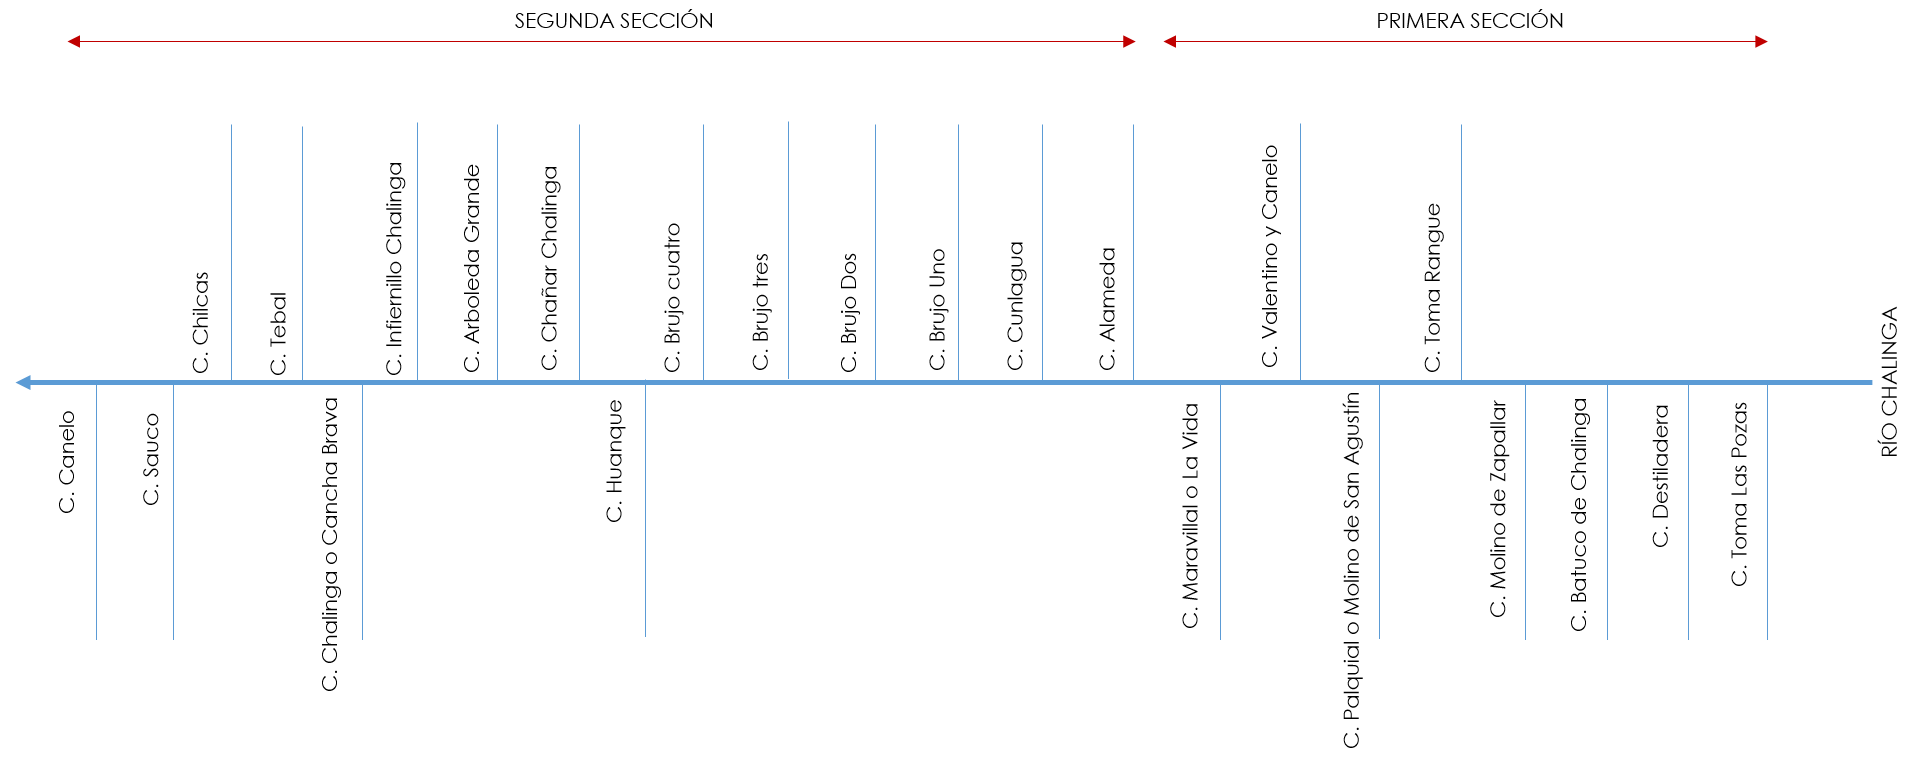
\includegraphics[width=\textwidth]{Logo/DiagramaChalinga}}
\caption{Diagrama Unifilar Junta de Vigilancia del Río Chalinga y sus Afluentes.}
\label{etiqueta_figura8}
\end{center}
\end{figure}

Se actualizaron los datos de acciones y capacidad de porteo a partir de la información levantada a la organización correspondiente (Junta de Vigilancia del Río Chalinga y sus Afluentes), de los canales:
\begin{itemize}

\item \textbf{Arboleda Grande}, con 98,76 acciones, equivalentes a 119 $l/s$.
\item \textbf{Chalinga o Cancha Brava}, con 104,93 acciones, equivalentes a 150 $l/s$.
\item \textbf{Huanque}, con 109,26 acciones, equivalentes a 140 $l/s$.\\

\end{itemize}

Se generó un escenario llamado \textit{Escenario Revestimiento}, el cual contiene la actualización del número de acciones asociada a los derechos nominales sobre el río Chalinga
y la pérdida por conducción equivalente a 0$\%$ \\
\\
Al correr tal escenario, el modelo muestra como el revestimiento de esta sección del río Chalinga, afecta de manera positiva la cobertura de la demanda agrícola, particularmente los cultivos anuales. Tal efecto muestra un 4$\%$ como promedio de mayor cobertura a lo largo de la serie temporal. Sin embargo, es en los momento de menor disponibilidad hídrica cuando los efectos son mayores, donde la cobertura aumenta en mas de un 10$\%$ en meses de mayor demanda.

\begin{figure}[H]
\begin{center}
\fbox{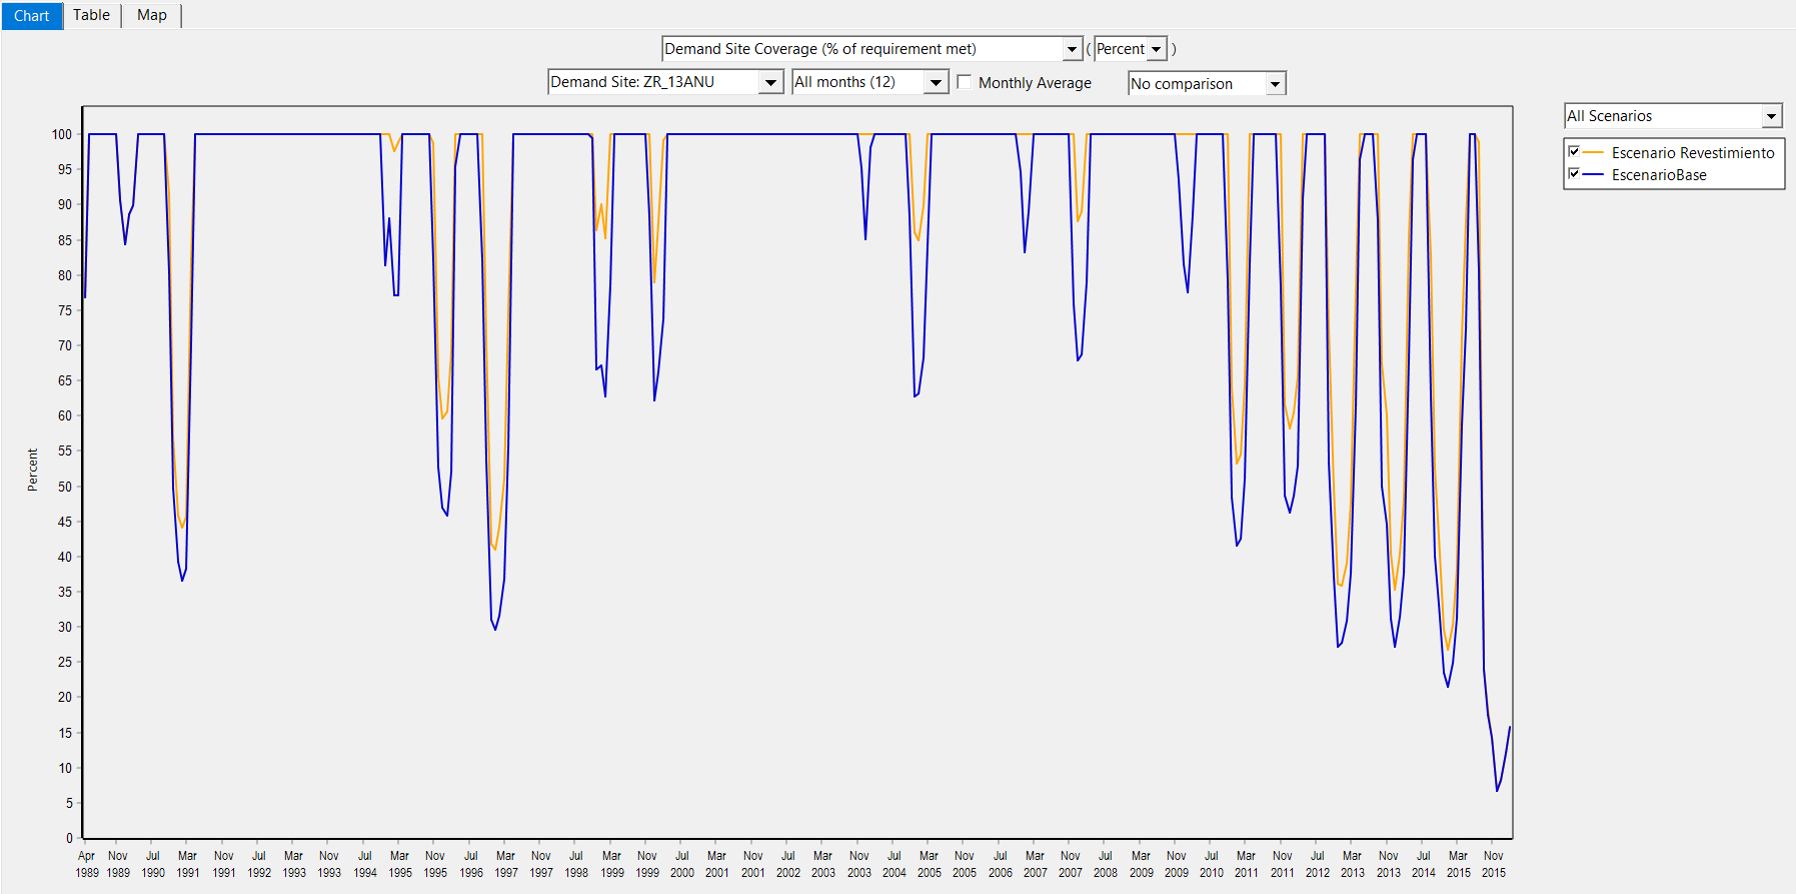
\includegraphics[width=\textwidth]{Logo/Validación1}}
\caption{Cobertura de la demanda de cultivos anuales ($\%$). Zona influenciada por los canales de la sección 2 del río Chalinga.}
\label{etiqueta_figura9}
\end{center}
\end{figure}

De igual manera la seguridad de la cobertura de la demanda de esta zona agrícola (cultivos anuales), sostuvo un aumento producto del revestimiento de sus canales a lo largo de la serie temporal. En el escenario base, la demanda fue satisfecha en un 100$\%$, el 68,5$\%$ de las oportunidades, mientras que en el escenario con revestimiento de canales, la seguridad aumentó a un 77,2\% (Figura \ref{etiqueta_figura10}).

\begin{figure}[H]
\begin{center}
\fbox{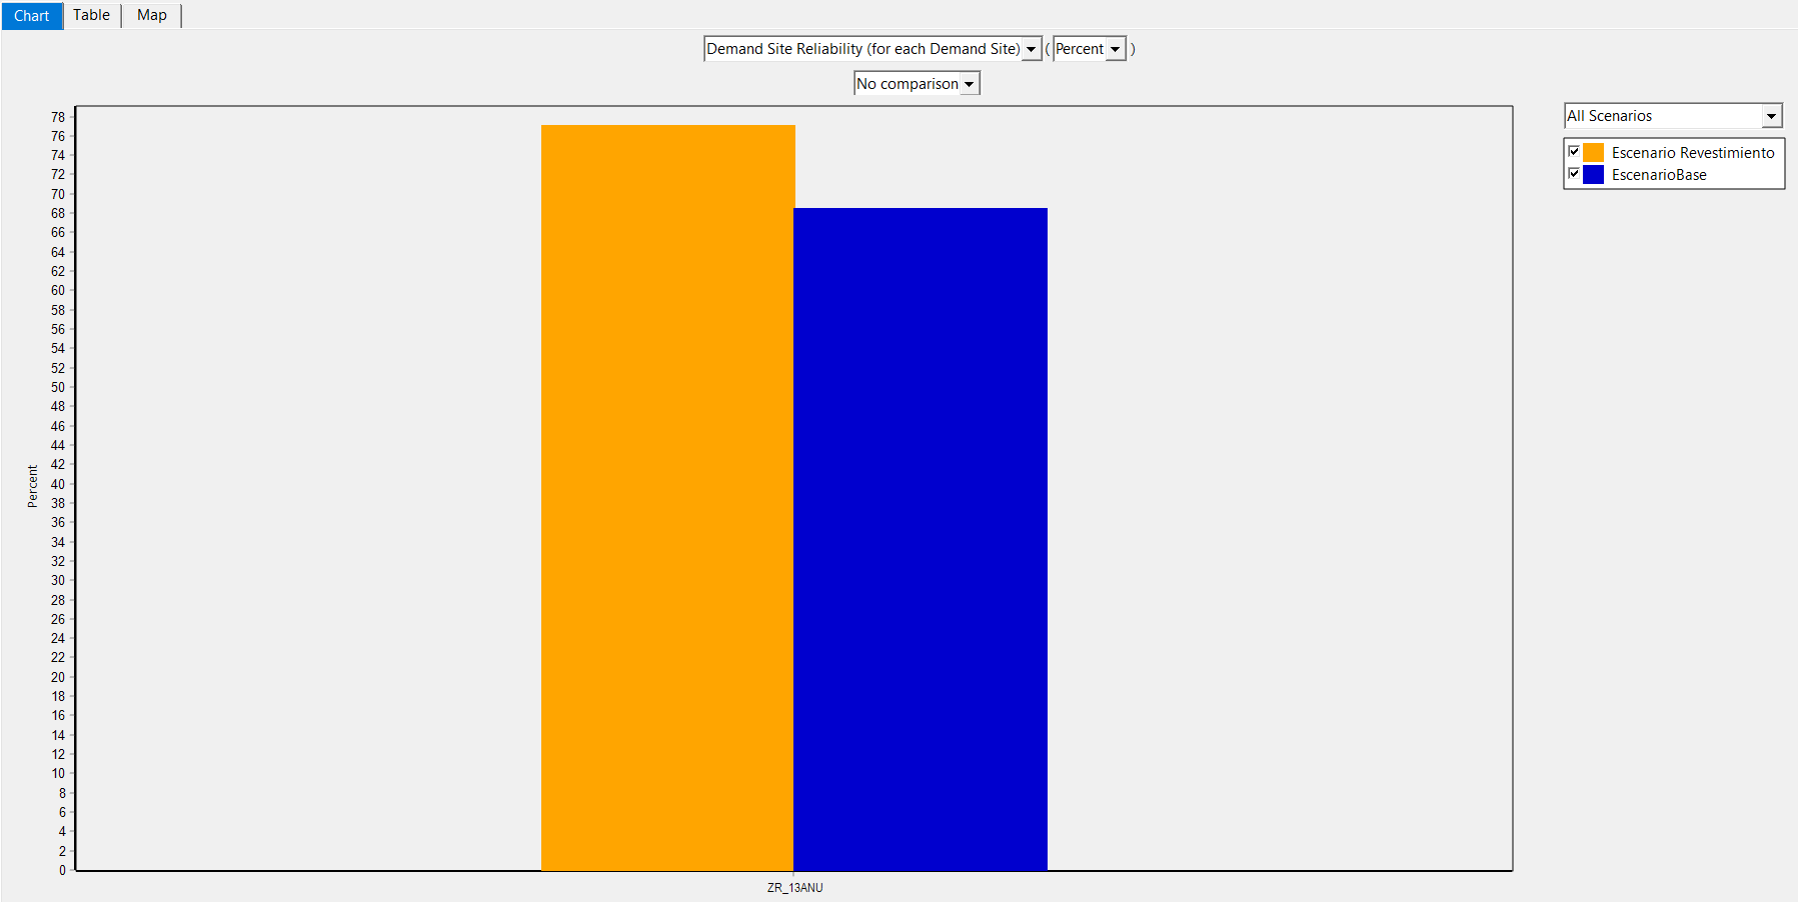
\includegraphics[width=\textwidth]{Logo/Validación2}}
\caption{Seguridad en la cobertura de la demanda de cultivos anuales ($\%$). Zona influenciada por los canales de la sección 2 del río Chalinga.}
\label{etiqueta_figura10}
\end{center}
\end{figure}

Los otros parámetros evaluados no tuvieron diferencias significativas entre ambos escenarios.


\subsubsection{Priorización de canales y tramos.}

La priorización de canales efectuada a los canales de validación, no consideró una clasificación en grupos de canales, ya que solo se dispone de 3 comunidades de aguas. Se realizó la matriz de las variables requeridas junto a las variables incorporadas de superficie (Cuadro \ref{tablav}). Posterior a esto se realizó un ordenamiento de las variables requeridas y variables de superficie, promediando los ordenamientos obtenemos el Plan de priorización (Cuadro \ref{tablaO}). La modelación hidrológica indica que los resultados de un mejoramiento en esta zona de la cuenca traería efectos positivos en la cobertura de la demanda agrícola y su seguridad. La priorización de tramos se realizará una vez que se obtenga todos los datos de la organización. 

\begin{landscape}
\begin{table} [H]
\centering
\caption{Variables requeridas por el Protocolo}
\label{tablav}
\begin{tabular}{|l|c|c|c|c|c|c|c|}
\hline
\textbf{Nombre Canal} & \textbf{N° Acciones} & \textbf{\begin{tabular}[c]{@{}c@{}}Capacidad de\\ porteo ($l/s$)\end{tabular}} & \textbf{\begin{tabular}[c]{@{}c@{}}N° de\\ Usuarios\end{tabular}} & \textbf{\begin{tabular}[c]{@{}c@{}}Superficie \\ bajo riego \\ ($ha$) \end{tabular}} & \textbf{\begin{tabular}[c]{@{}c@{}}Superficie \\ potencial\\ ($ha$) \end{tabular}} & \textbf{\begin{tabular}[c]{@{}c@{}}Volumen \\ recuperado \\ ($m^3/temporada$) \end{tabular}} & \textbf{\begin{tabular}[c]{@{}c@{}}Volumen recuperado \\ por $m^2$ a revestir\\ ($m^3/m^2 de revestido$) \end{tabular}} \\ \hline
Chalinga  		& 104,93 & 165 & 85 & 13,07 & 40 & 911075,0 & 167,4 \\ \hline
Arboleda Grande & 98,78 & 129,9 & 160 & 17,71 & 46,76 & 1368662,4 & 398,1 \\ \hline
Huanque			& 109,26 & 154 & 97 & 11,80 & 56,71 & 504576,0 & 157,0 \\ \hline
\end{tabular}
\end{table}

\begin{table} [H]
\centering
\caption{Ordenamiento por variables requeridas por el Protocolo}
\label{tablaO}
\begin{tabular}{|l|c|c|c|c|c|c|c|c|}
\hline
\textbf{Nombre Canal} & \textbf{N° Acciones} & \textbf{\begin{tabular}[c]{@{}c@{}}Capacidad de\\ porteo ($l/s$)\end{tabular}} & \textbf{\begin{tabular}[c]{@{}c@{}}N° de\\ Usuarios\end{tabular}} & \textbf{\begin{tabular}[c]{@{}c@{}}Superficie \\ bajo riego \\ ($ha$) \end{tabular}} & \textbf{\begin{tabular}[c]{@{}c@{}}Superficie \\ potencial\\ ($ha$) \end{tabular}} & \textbf{\begin{tabular}[c]{@{}c@{}}Volumen \\ recuperado \\ ($m^3/temporada$) \end{tabular}} & \textbf{\begin{tabular}[c]{@{}c@{}}Volumen recuperado \\ por $m^2$ a revestir\\ ($m^3/m^2 de revestido$) \end{tabular}} & \textbf{Priorización} \\ \hline
Chalinga  		& 2 & 1 & 3 & 2 & 3 & 2 & 2 & 2 \\ \hline
Arboleda Grande & 3 & 3 & 1 & 1 & 2 & 1 & 1 & 1 \\ \hline
Huanque			& 1 & 2 & 2 & 3 & 1 & 3 & 3 & 2 \\ \hline
\end{tabular}
\end{table}
\end{landscape}


\subsection{Resultados Actividades de Difusión}



\clearpage
\section{Impactos logrados a la fecha.}

\clearpage
\section{Problemas enfrentados.}

\clearpage
\section{Programa del próximo período.}

\clearpage
\section{Conclusiones y recomendaciones.}

\clearpage
\section{Anexos. Componente 1.}

\textbf{- Comunidad de Aguas Chalinga o Cancha Brava.}

\begin{figure}[H]
  \centering
\begin{subfigure}{.45\textwidth}
\hfill
  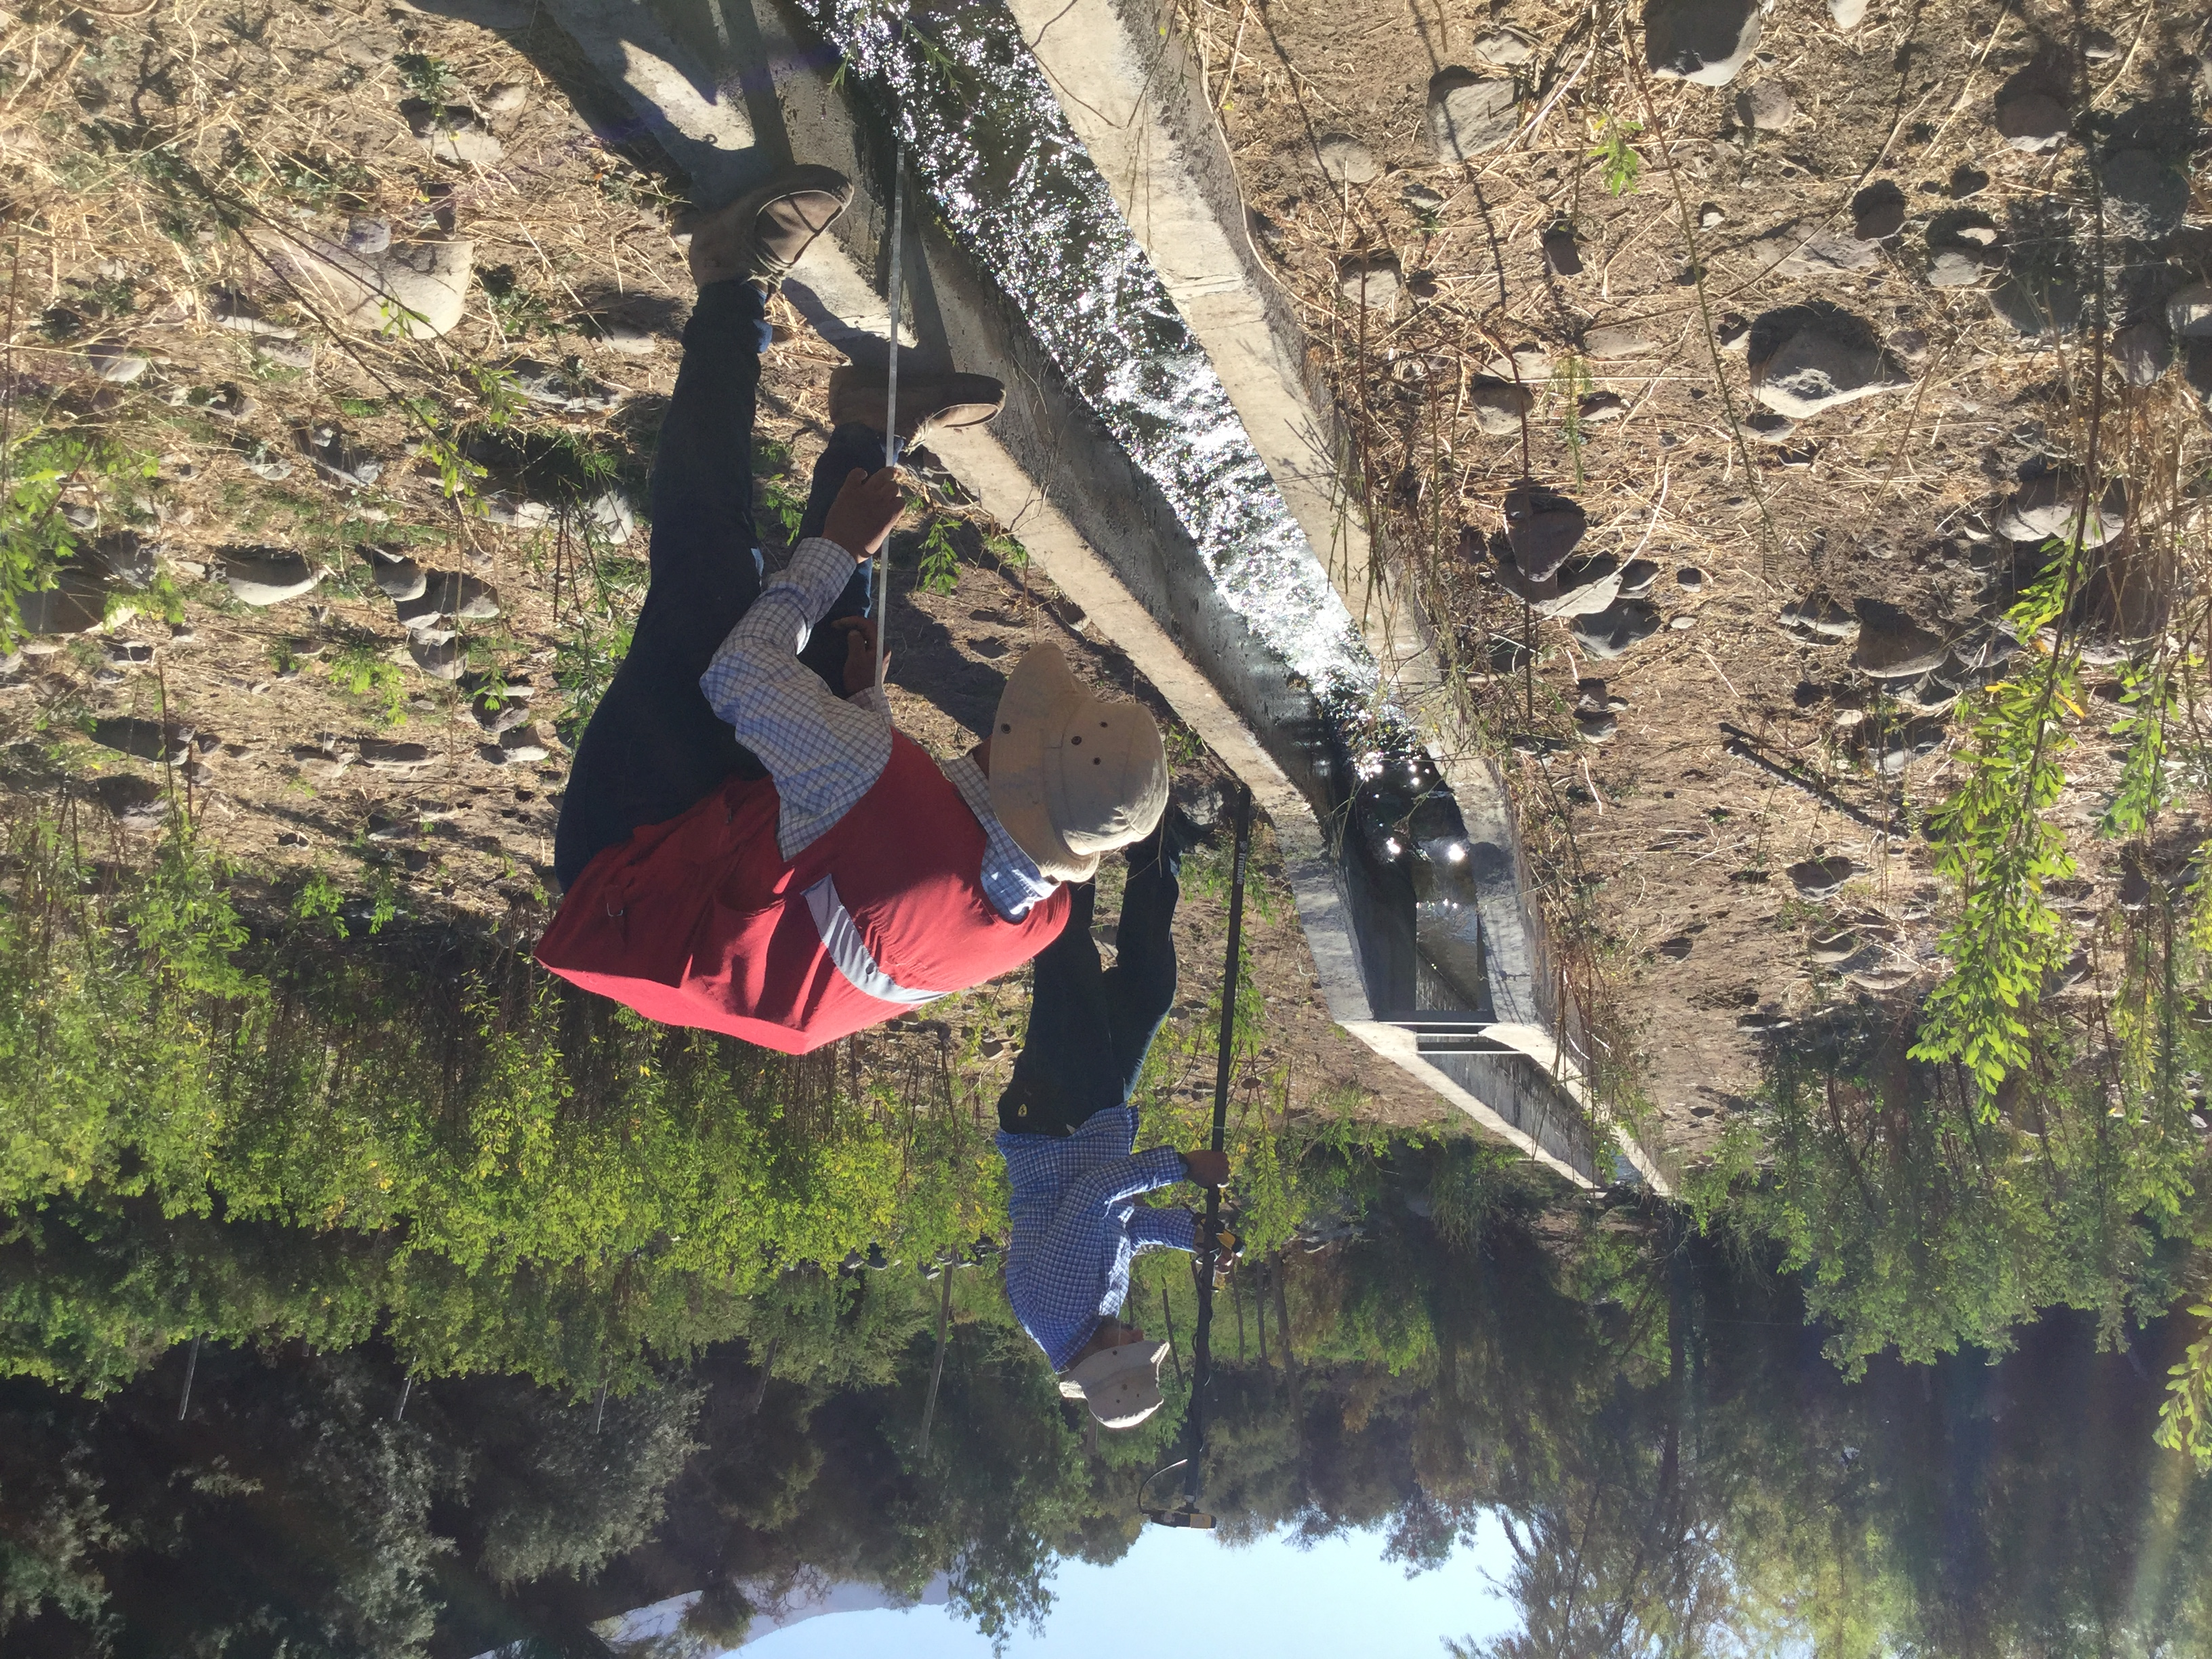
\includegraphics[angle= 180, width=\textwidth]{Foto/ch1.jpg}
\end{subfigure}
\hfill
\begin{subfigure}{.45\textwidth}
\hfill
  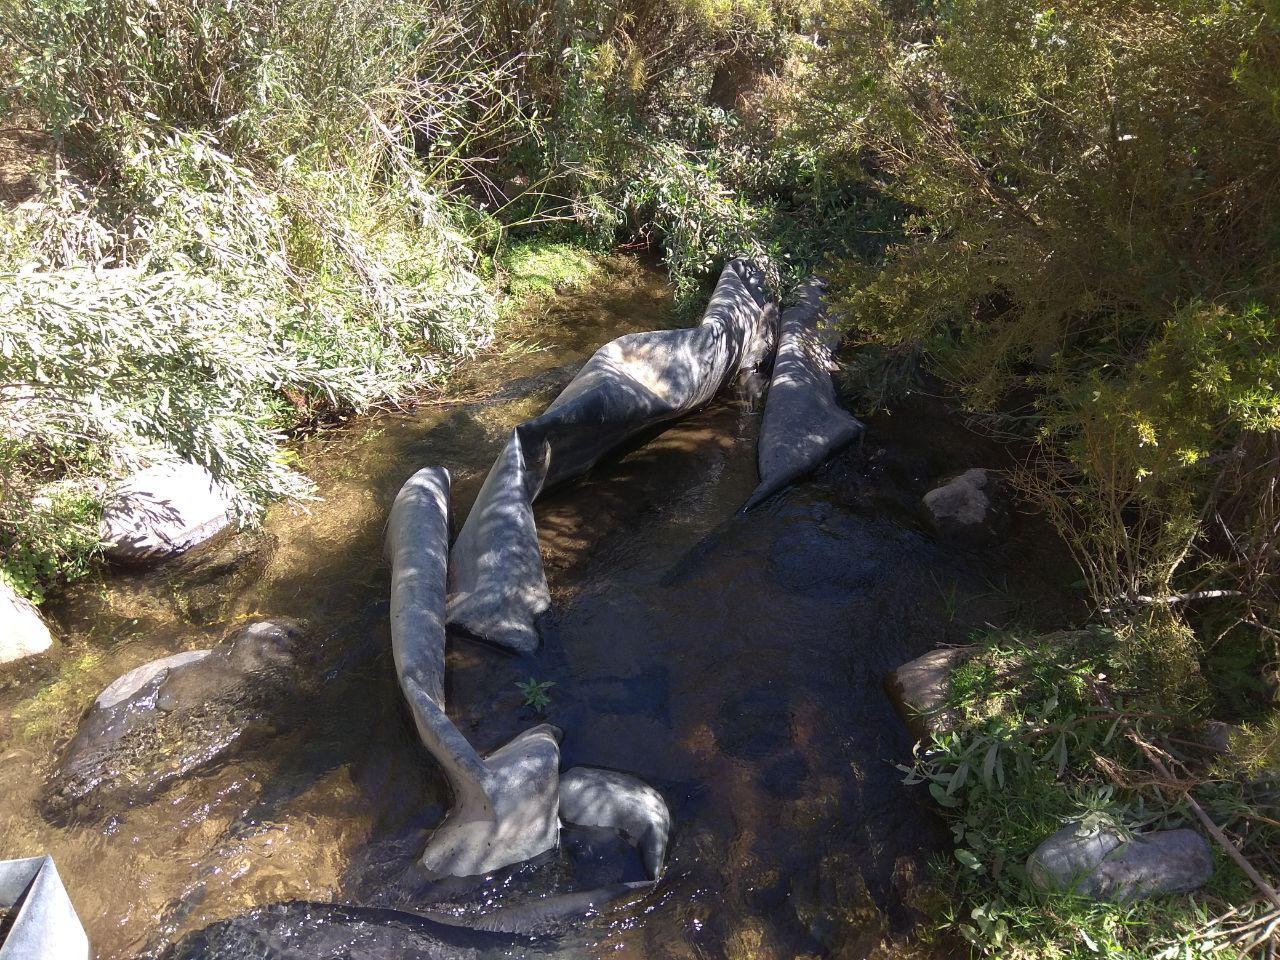
\includegraphics[width=\textwidth]{Foto/ch2.jpg} 
\end{subfigure}
\caption{Caracterización de infraestructura hídrica para el S.I.G. de Canal Chalinga o Cancha Brava, cuenca del río Chalinga.}
\end{figure}

\begin{figure}[H]
  \centering
\begin{subfigure}{.45\textwidth}
\hfill
  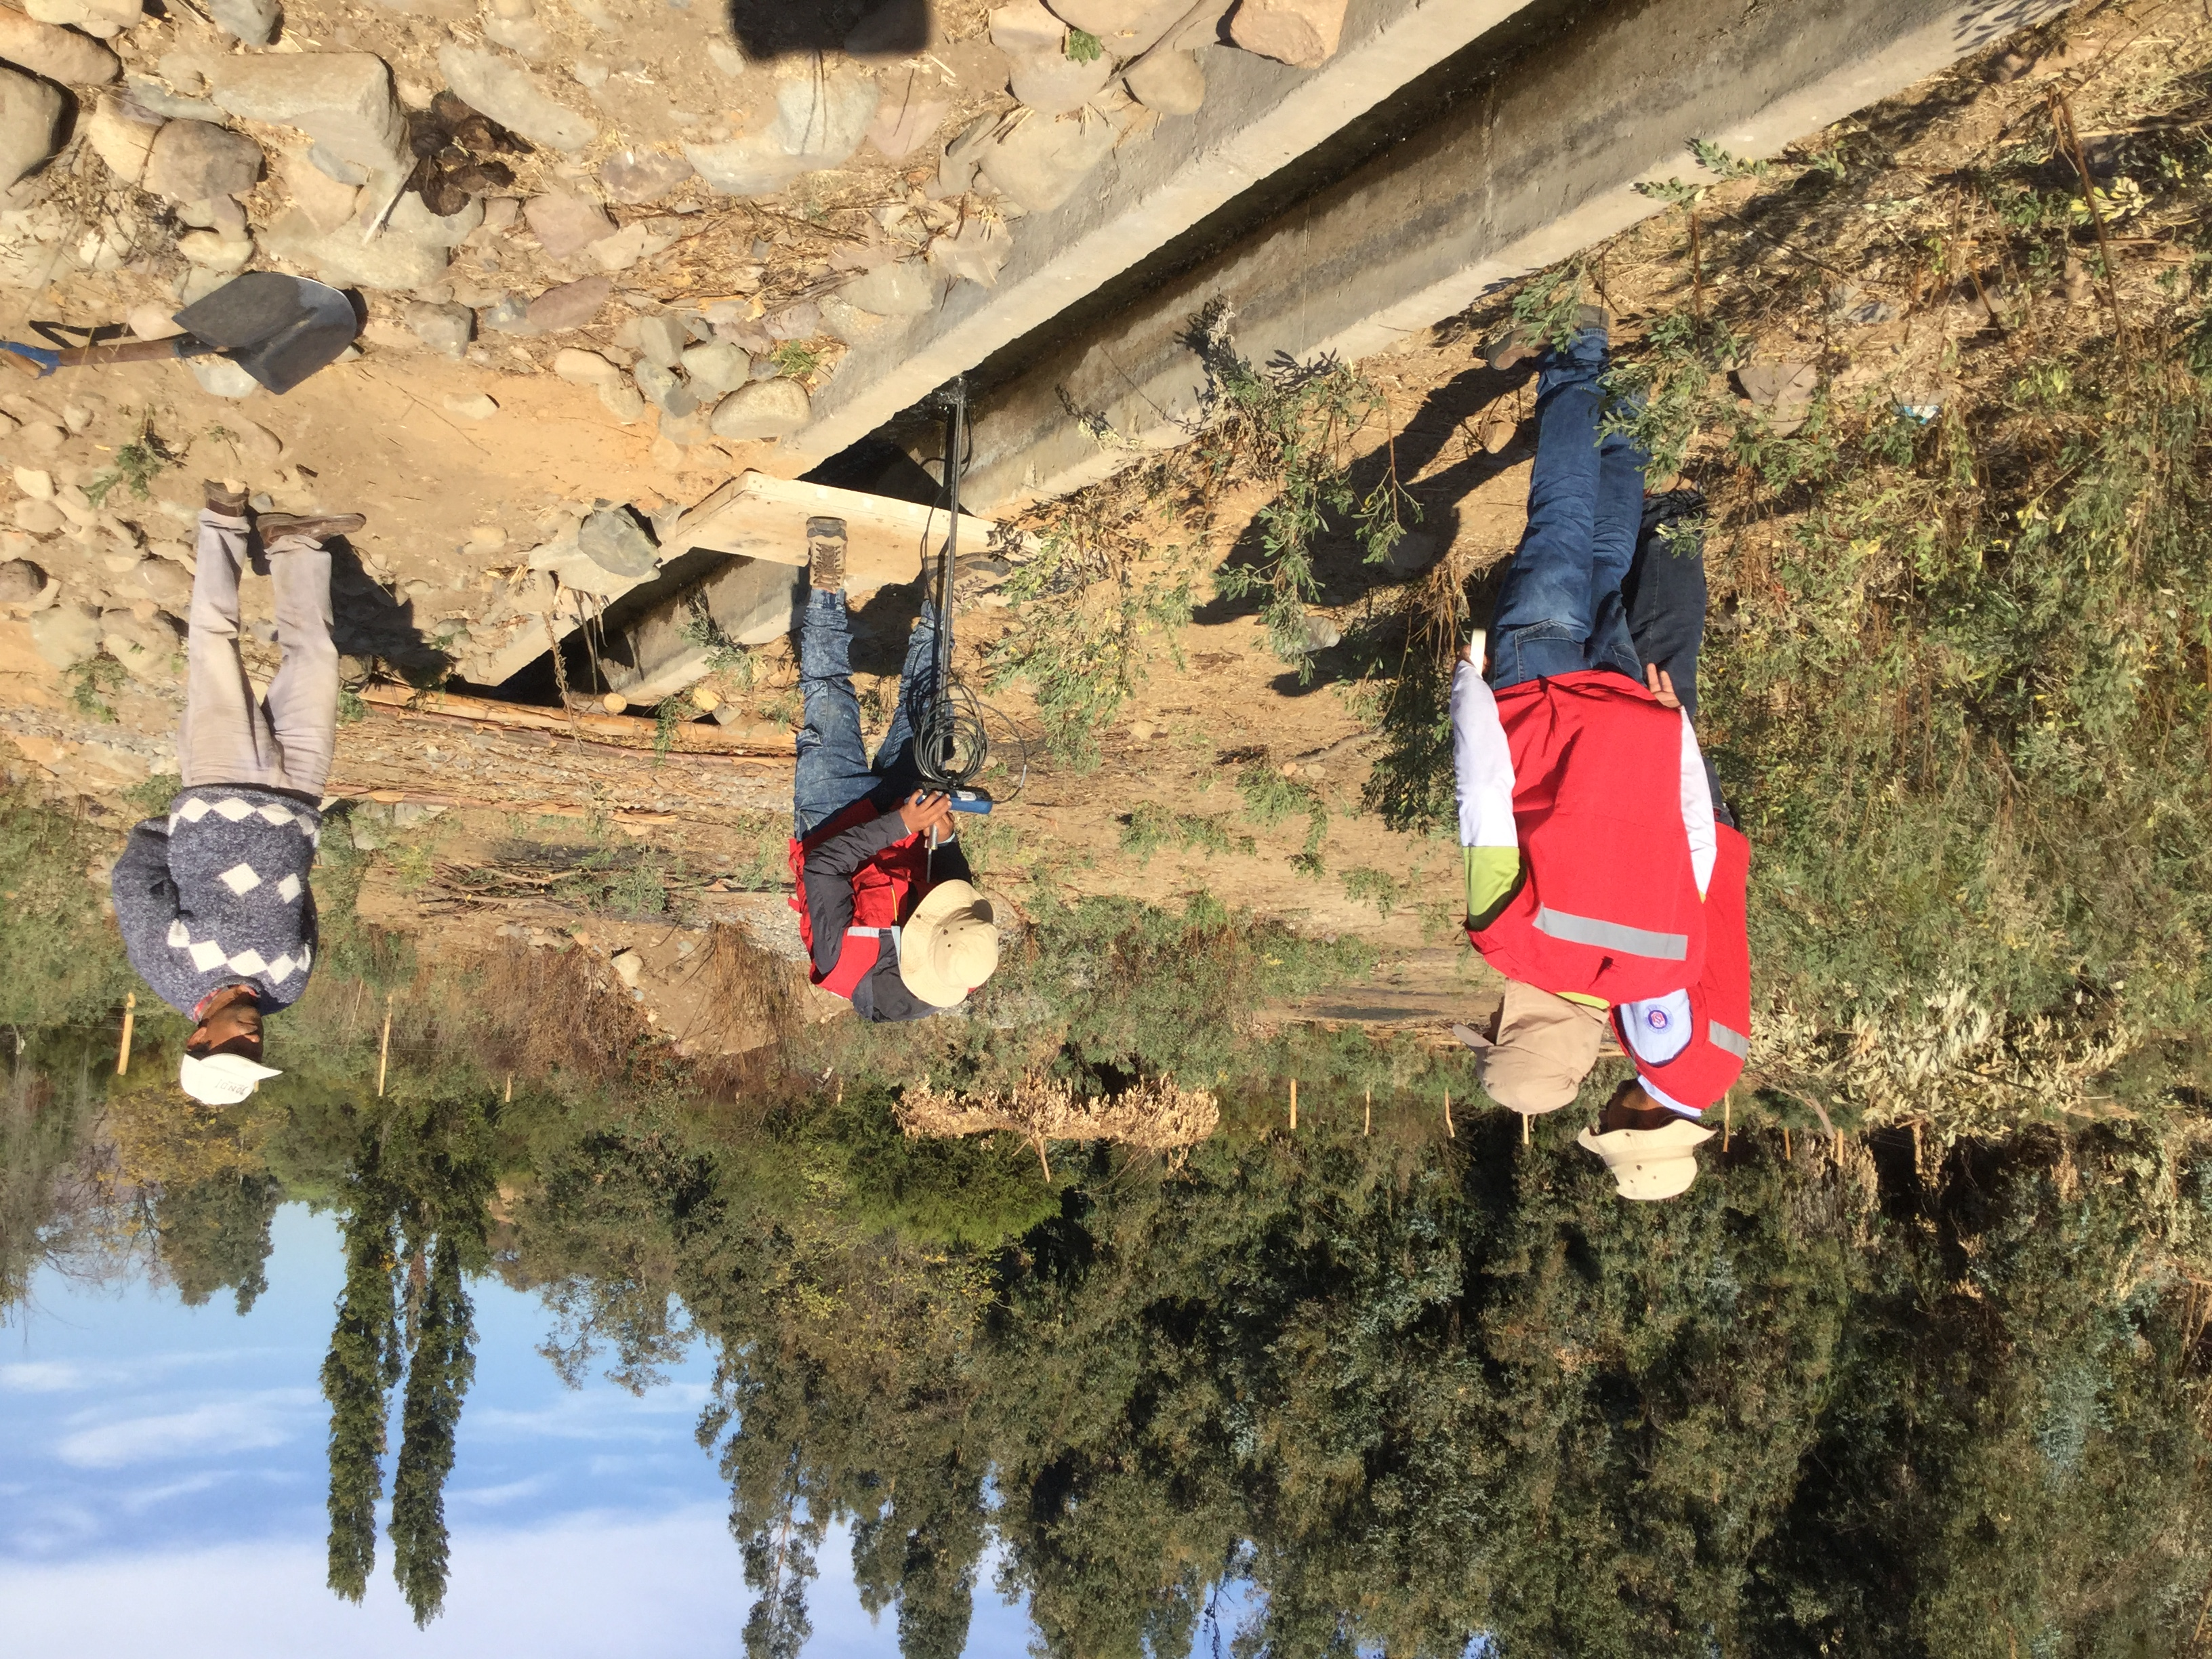
\includegraphics[angle= 180, width=\textwidth]{Foto/ch3.jpg}
\end{subfigure}
\hfill
\begin{subfigure}{.45\textwidth}
\hfill
  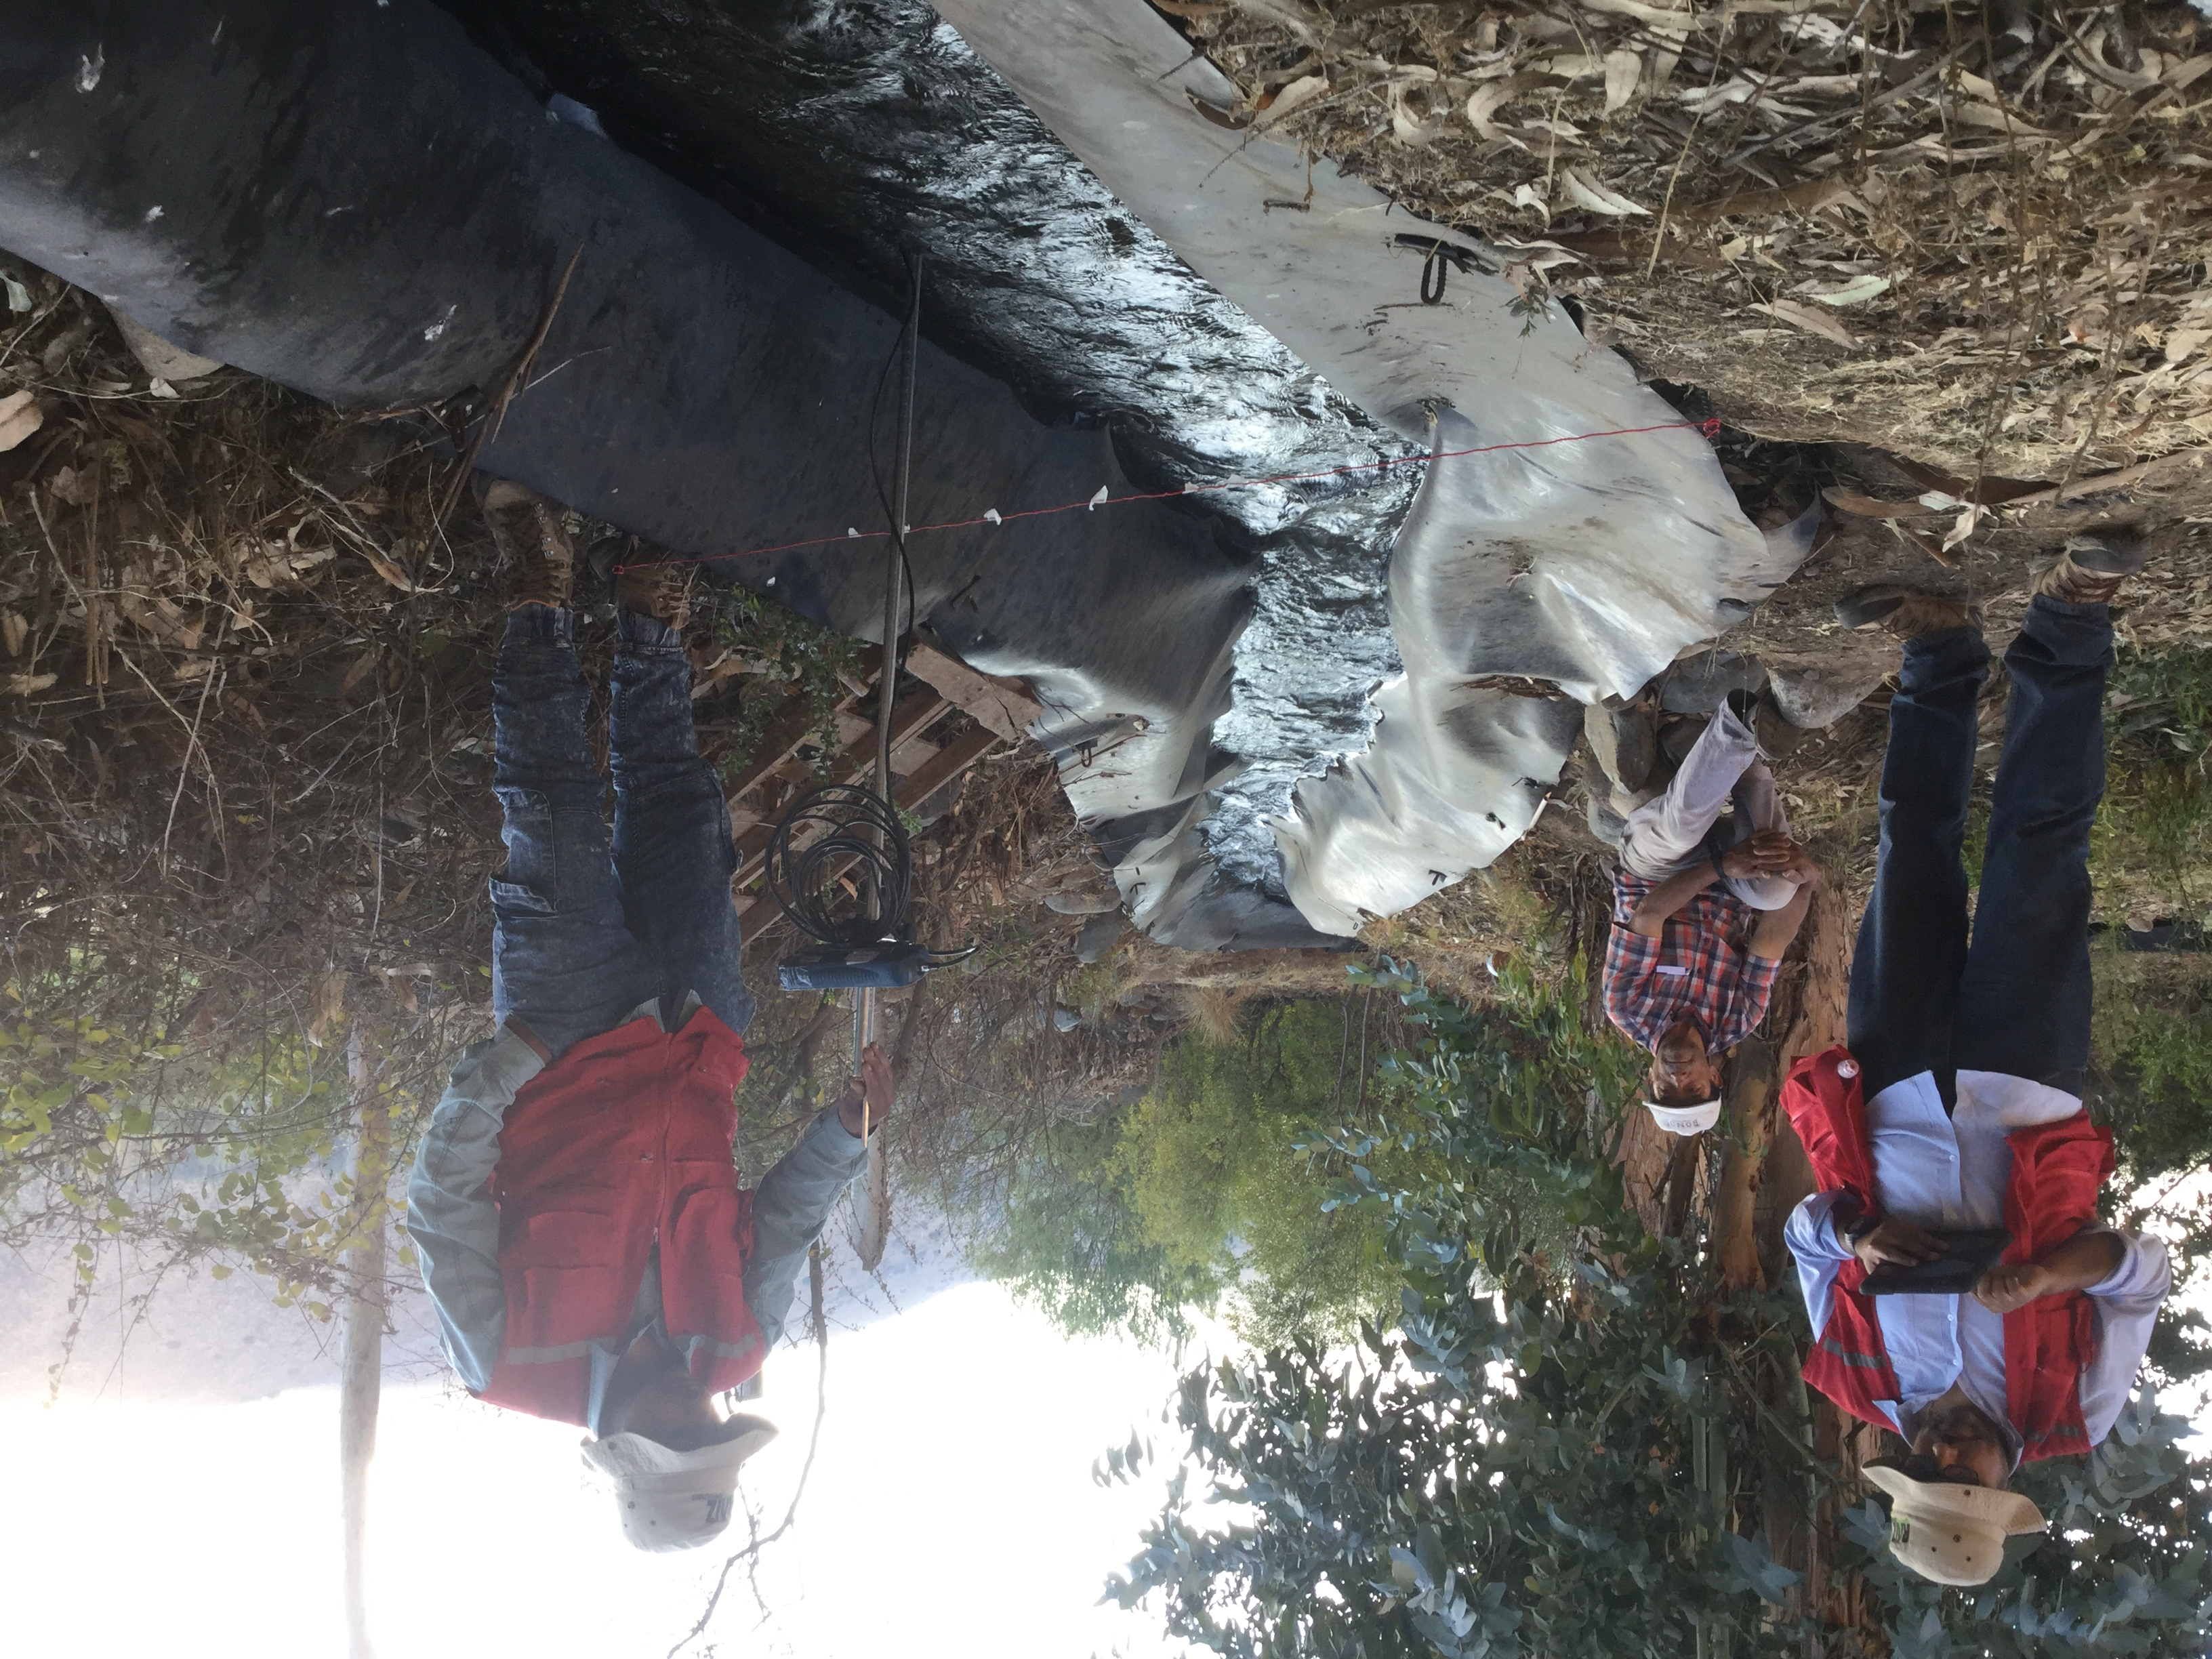
\includegraphics[angle= 180, width=\textwidth]{Foto/ch4.jpg} 
\end{subfigure}
\caption{Aforos de caudal Canal Chalinga o Cancha Brava, cuenca río Chalinga.}
\end{figure}
\clearpage

\textbf{- Comunidad de Aguas Arboleda Grande.}

\begin{figure}[H]
  \centering
\begin{subfigure}{.45\textwidth}
\hfill
  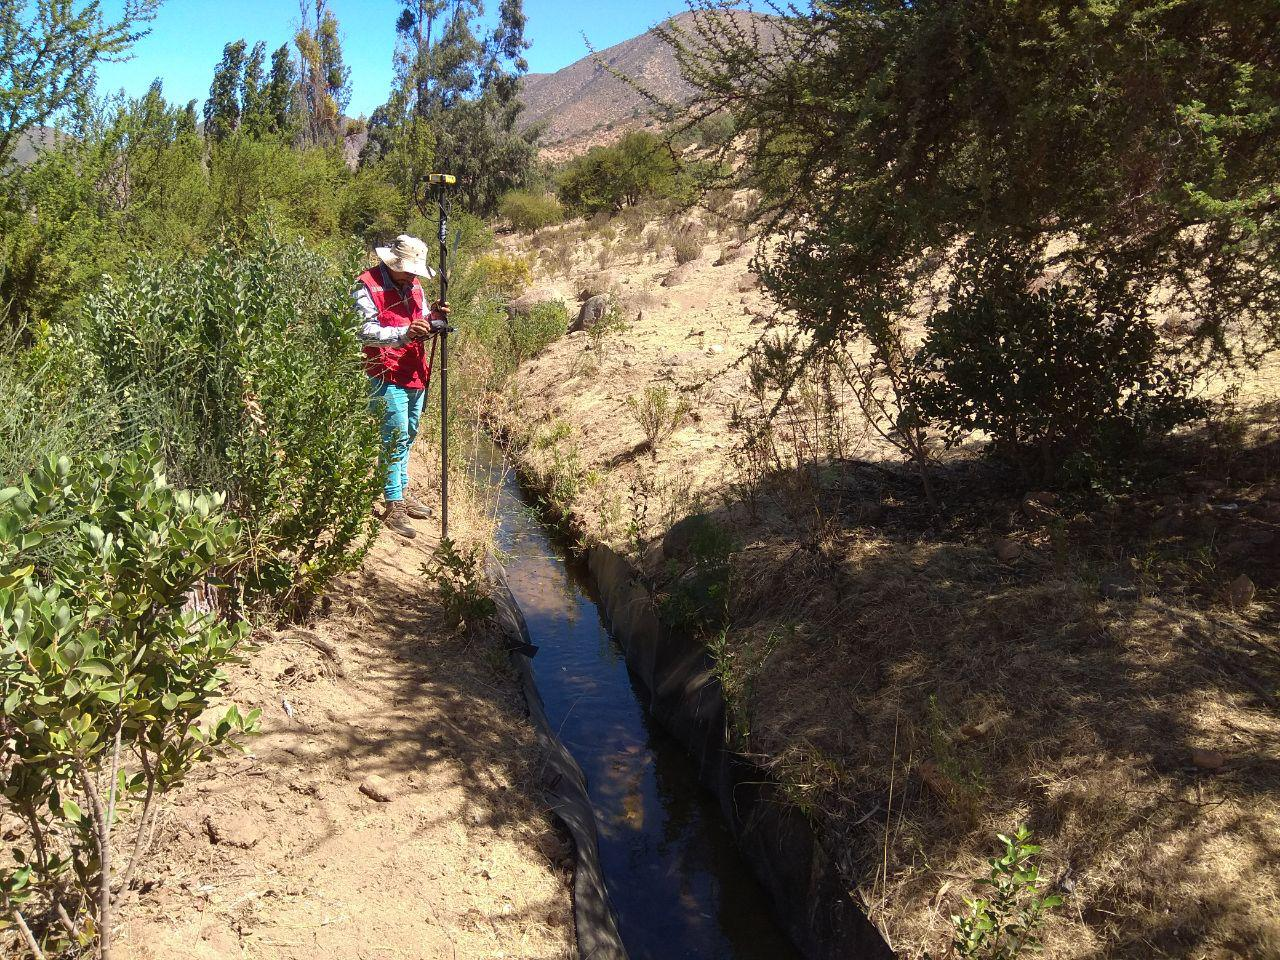
\includegraphics[width=\textwidth]{Foto/a1.jpg}
\end{subfigure}
\hfill
\begin{subfigure}{.45\textwidth}
\hfill
  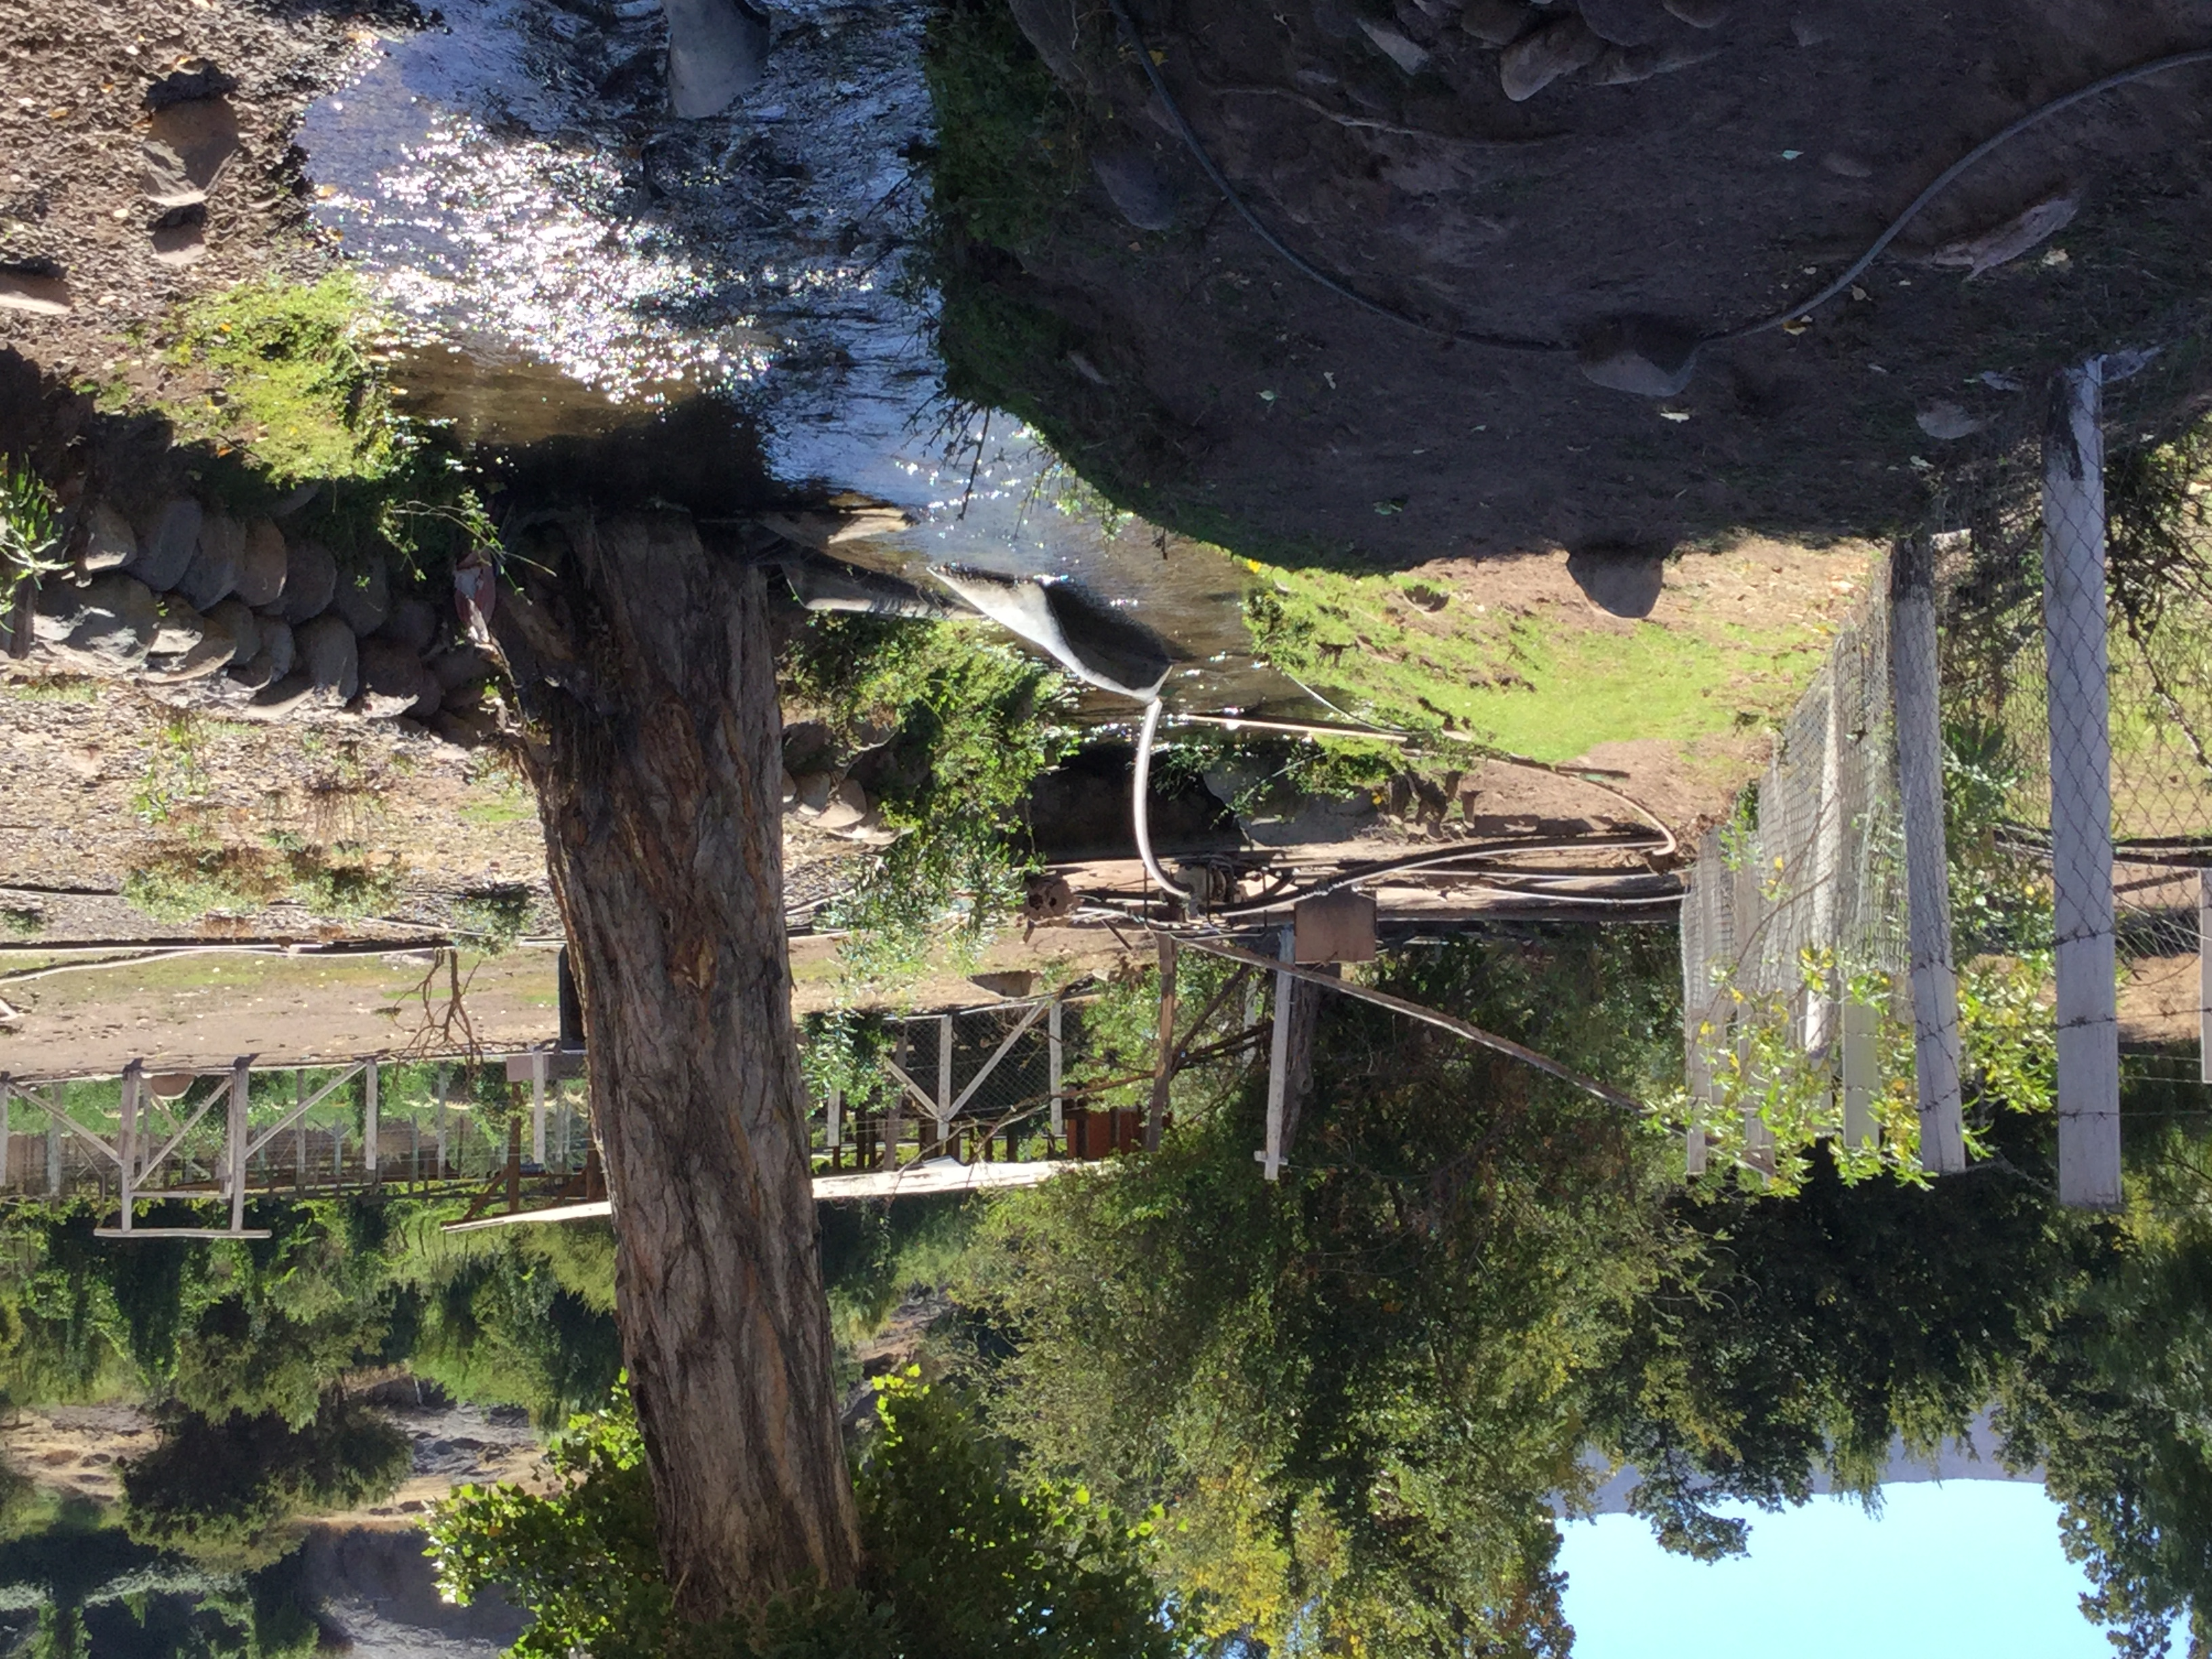
\includegraphics[angle= 180, width=\textwidth]{Foto/a2.jpg} 
\end{subfigure}
\caption{Caracterización de infraestructura hídrica para el S.I.G. de Canal Arboleda Grande, cuenca río Chalinga.}
\end{figure}

\begin{figure}[H]
  \centering
\begin{subfigure}{.45\textwidth}
\hfill
  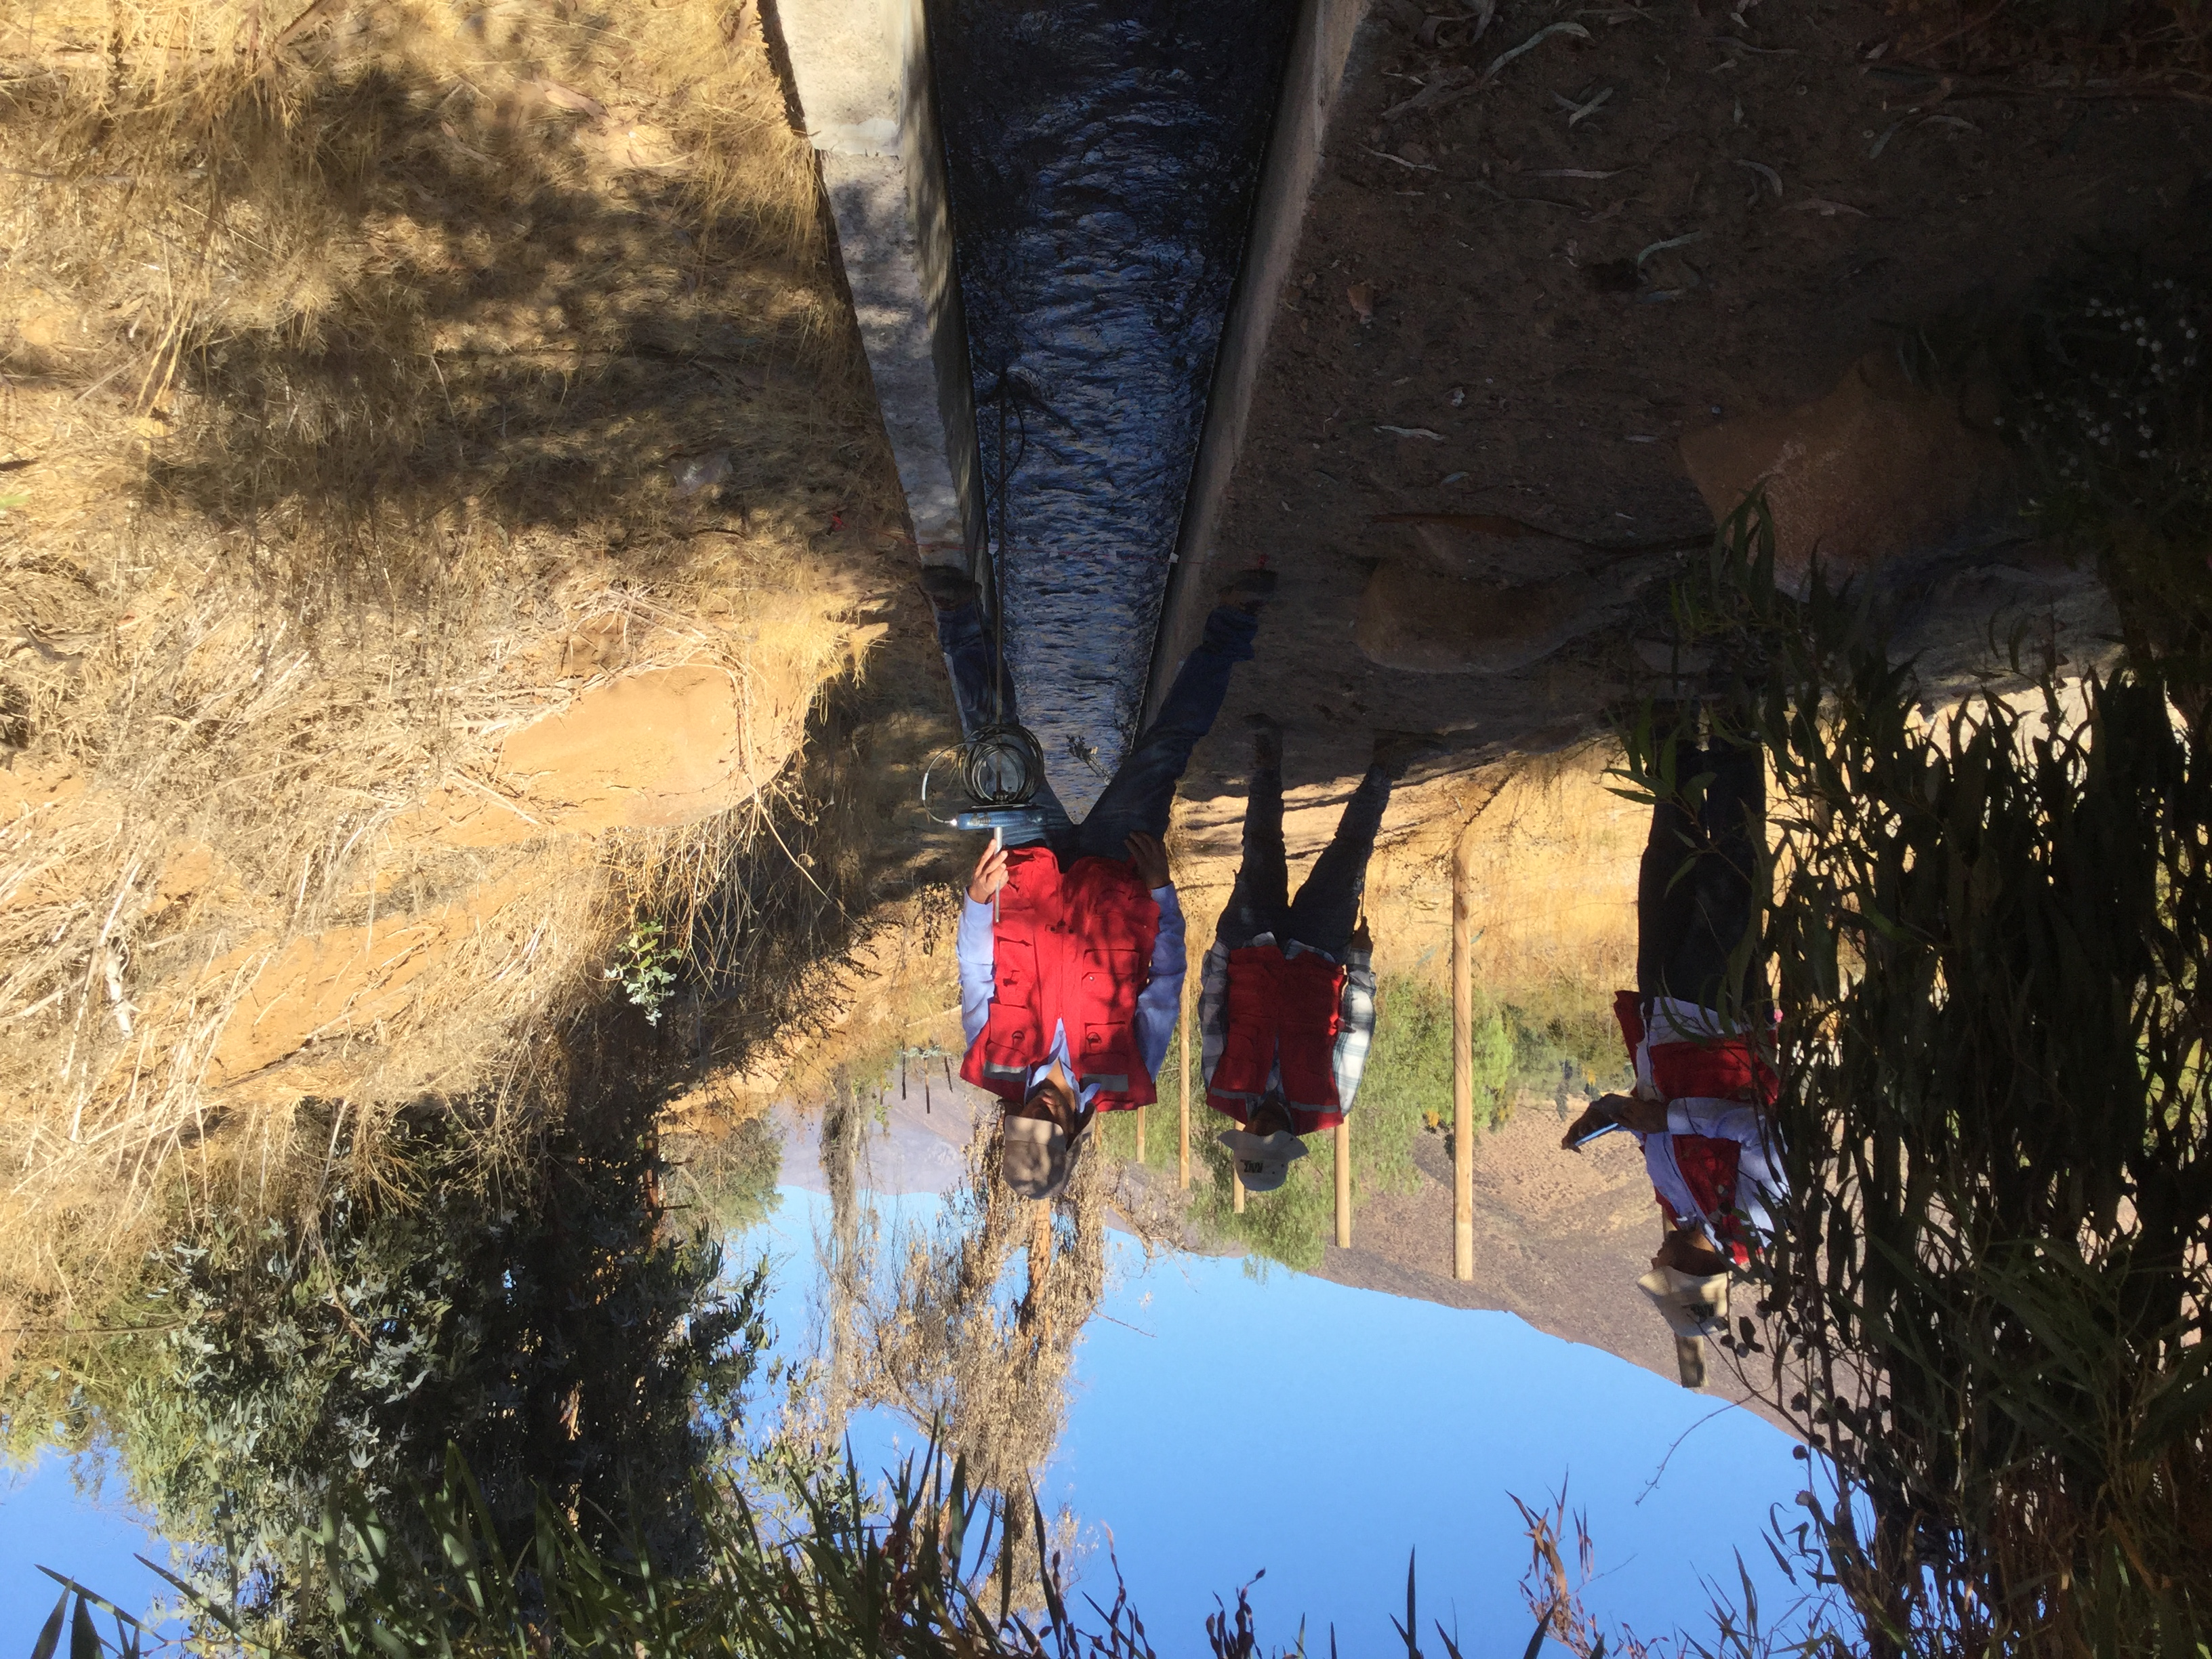
\includegraphics[angle= 180, width=\textwidth]{Foto/a3.jpg}
\end{subfigure}
\hfill
\begin{subfigure}{.45\textwidth}
\hfill
  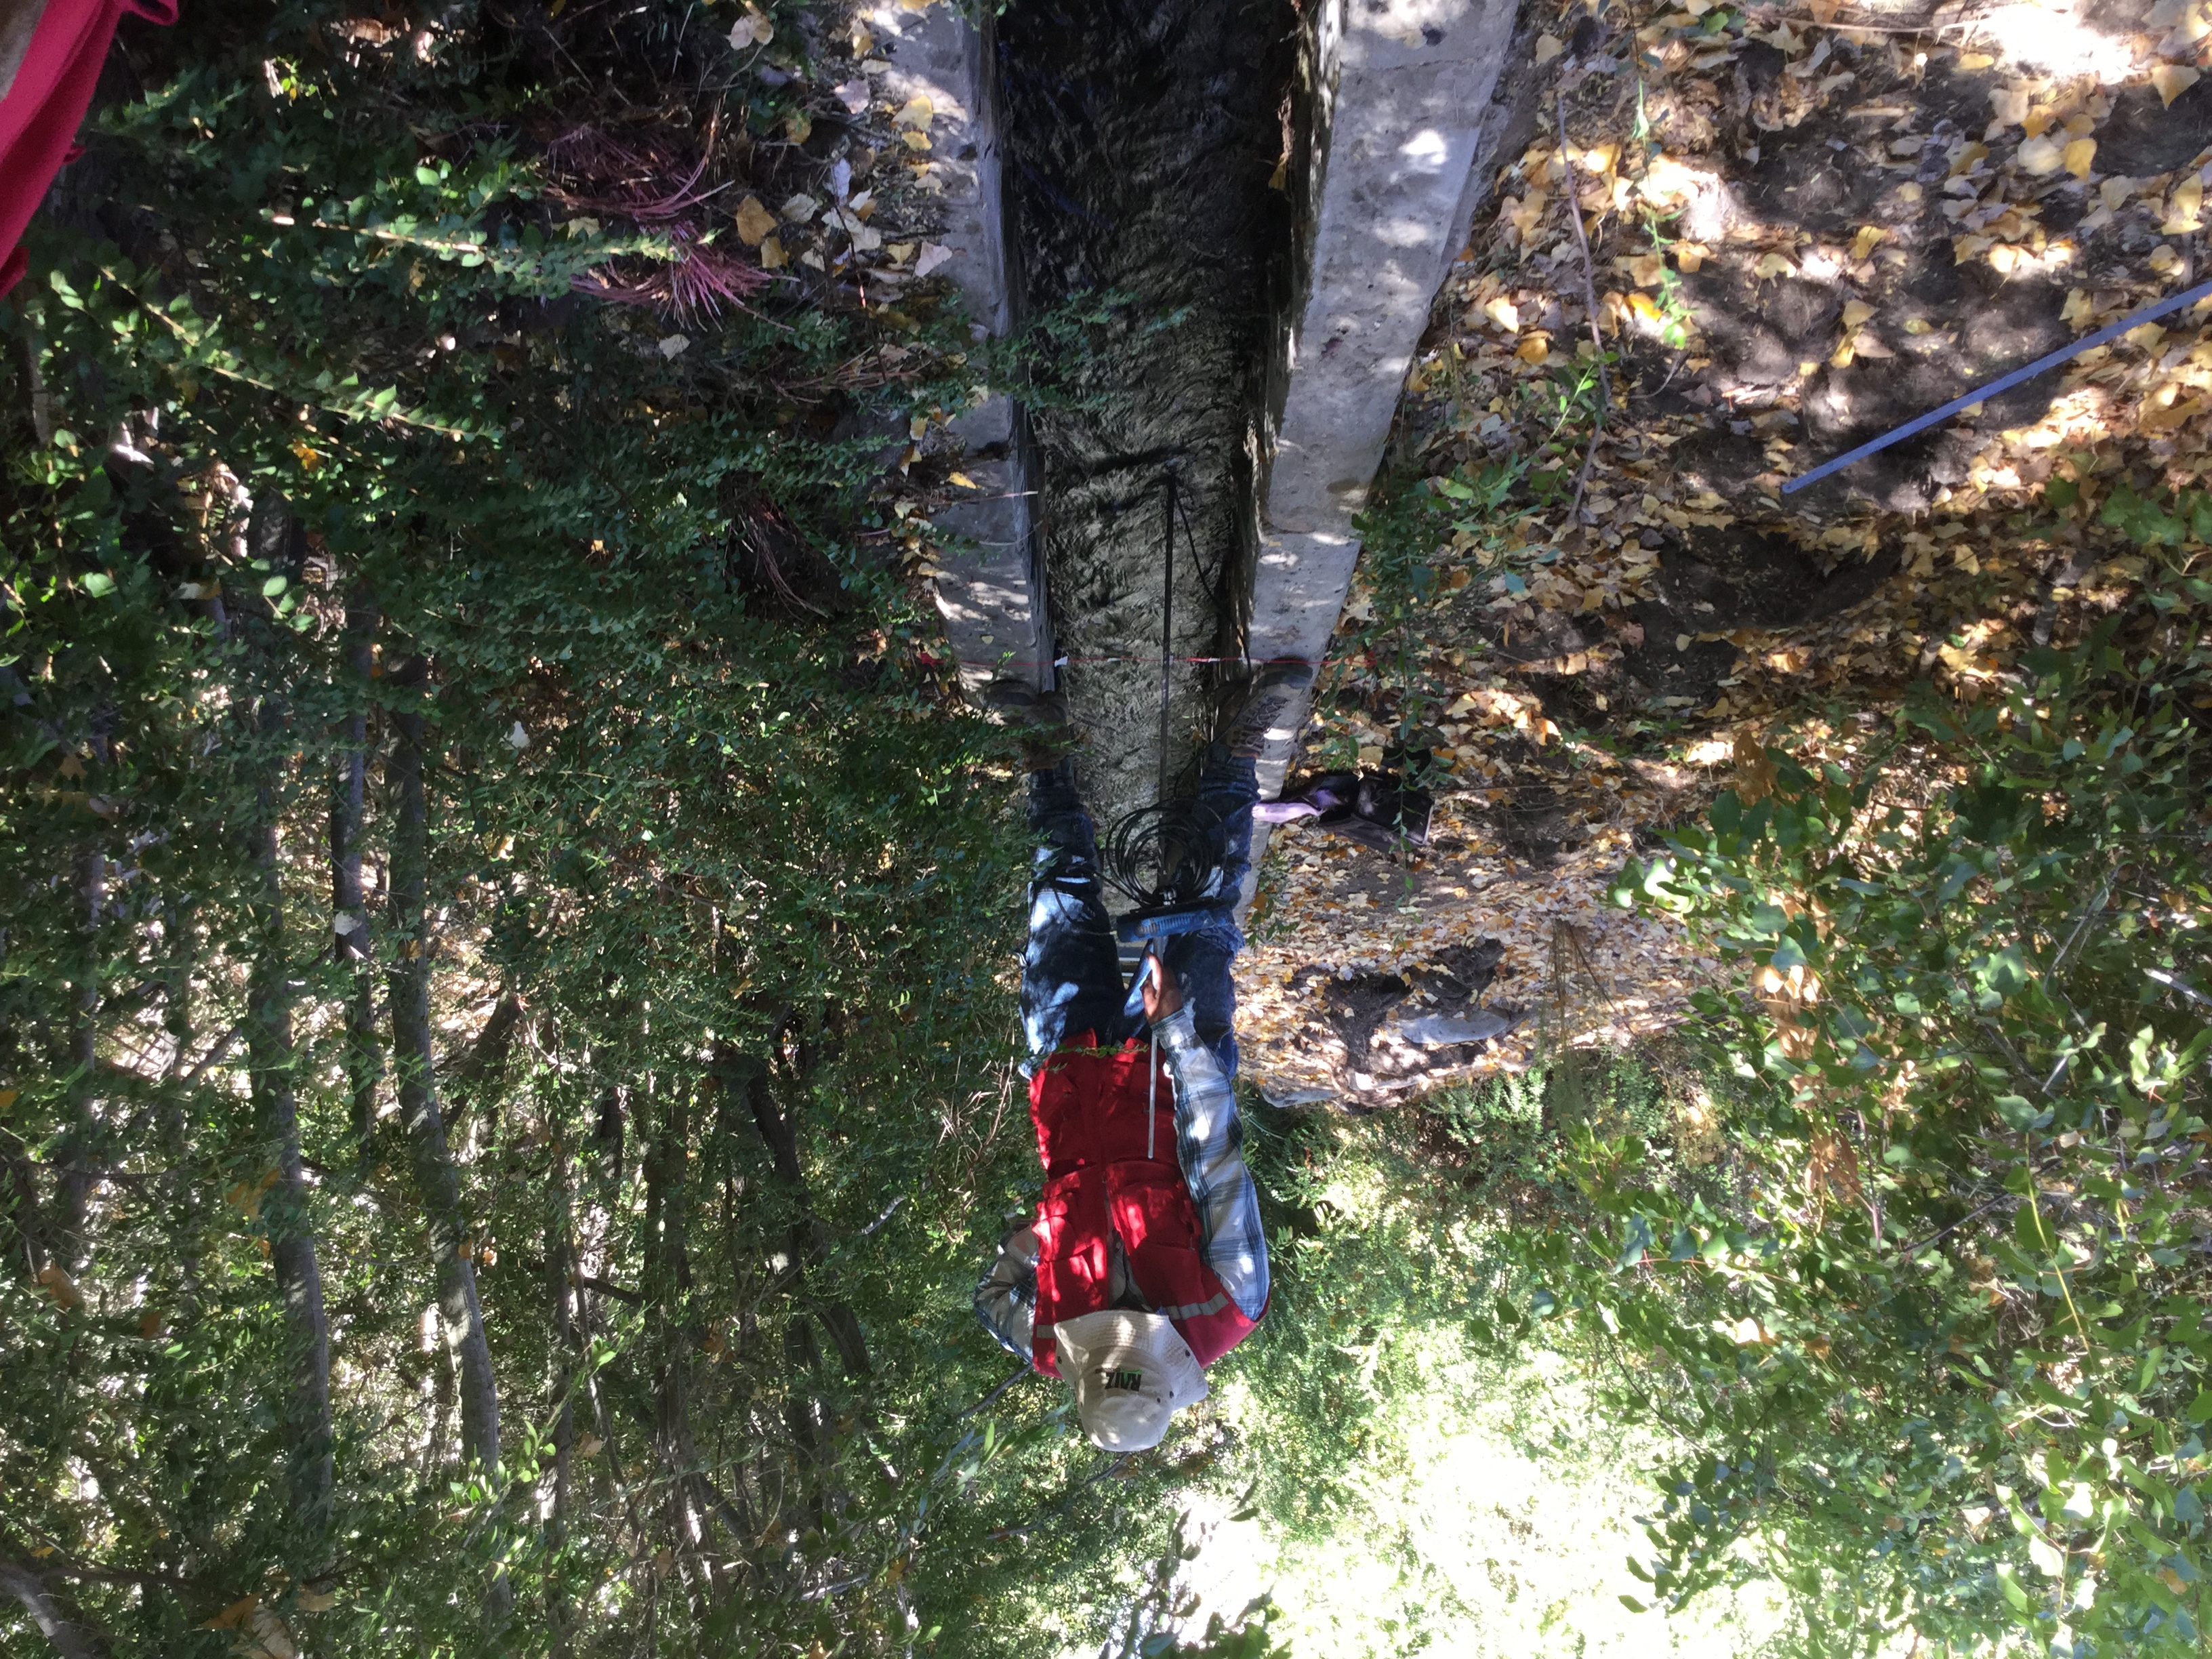
\includegraphics[angle= 180, width=\textwidth]{Foto/a4.jpg} 
\end{subfigure}
\caption{Aforos de caudal Canal Arboleda Grande, cuenca río Chalinga.}
\end{figure}
\clearpage

\textbf{- Comunidad de aguas Huanque.}

\begin{figure}[H]
  \centering
\begin{subfigure}{.45\textwidth}
\hfill
  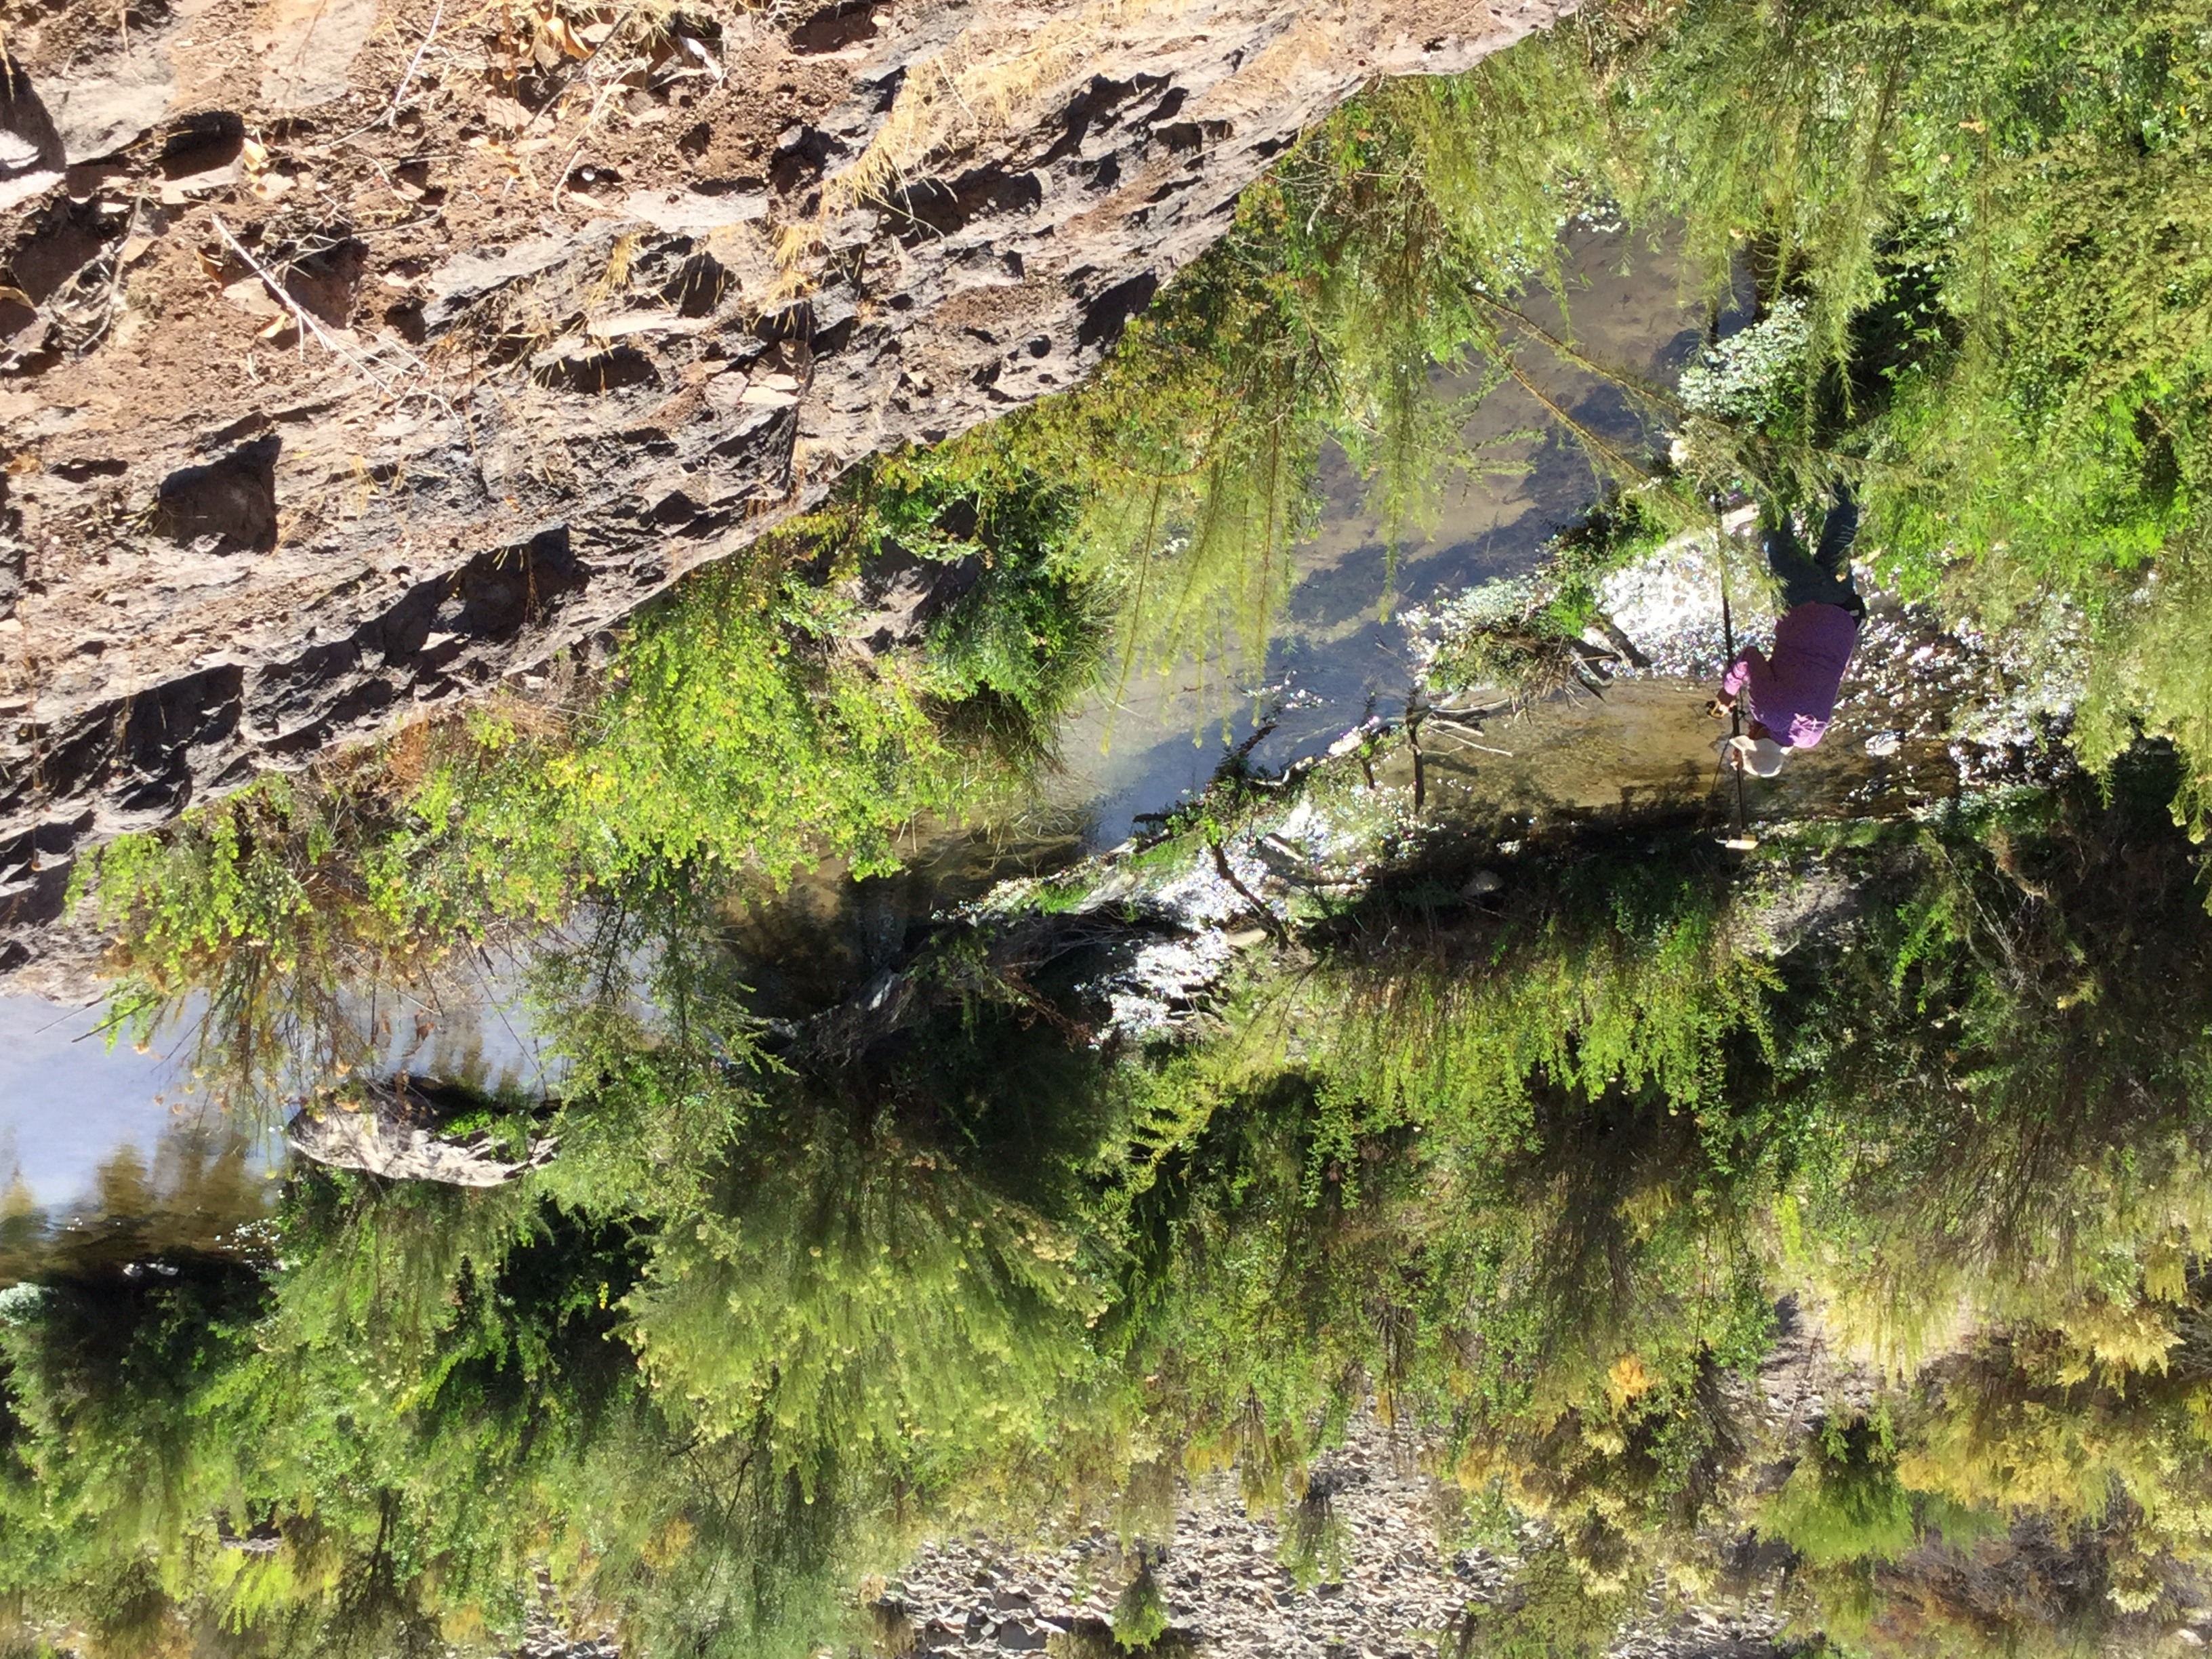
\includegraphics[angle= 180, width=\textwidth]{Foto/h1.jpg}
\end{subfigure}
\hfill
\begin{subfigure}{.45\textwidth}
\hfill
  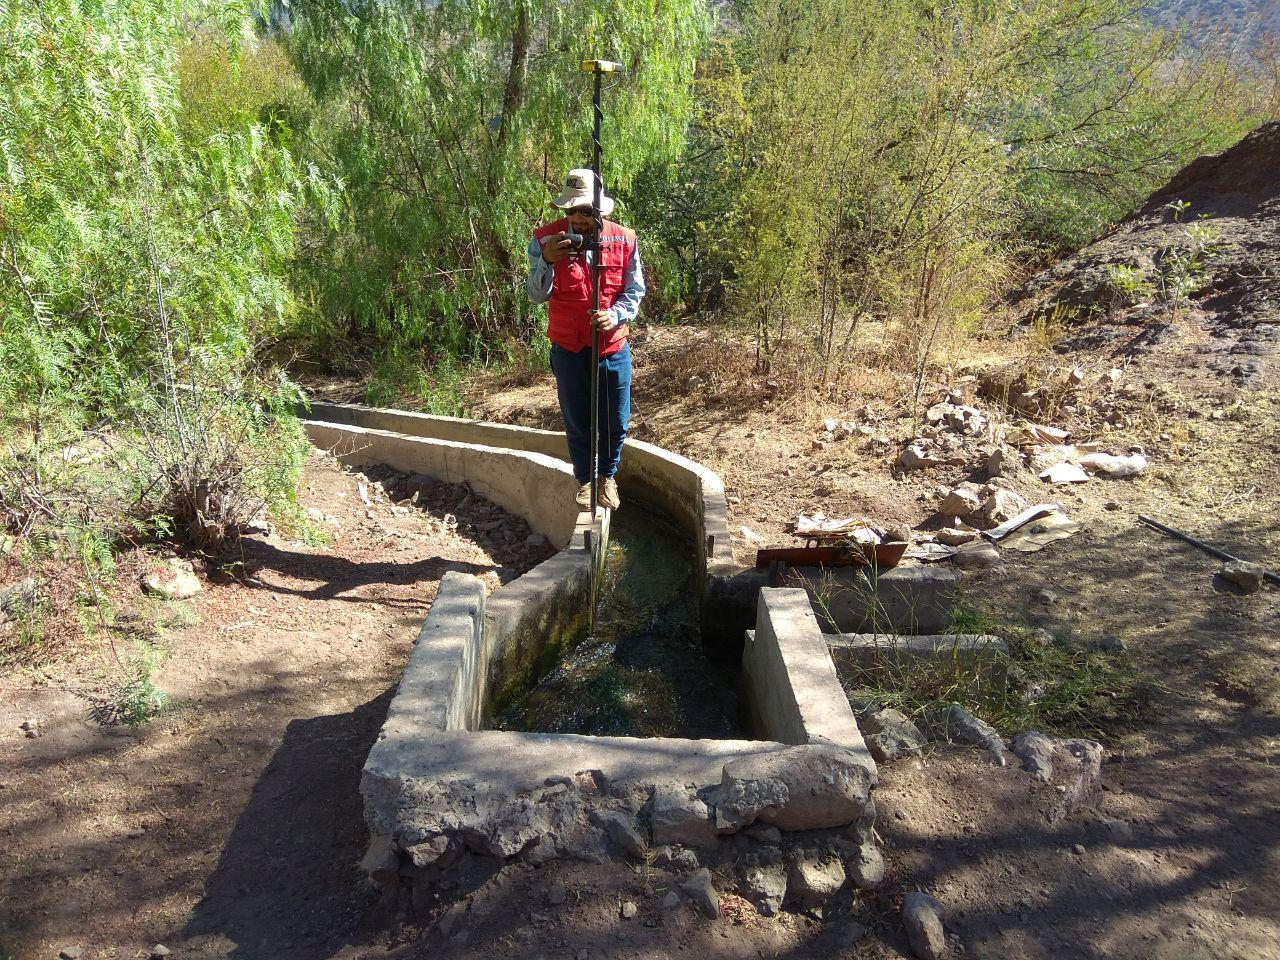
\includegraphics[width=\textwidth]{Foto/h2.jpg} 
\end{subfigure}
\caption{Caracterización de infraestructura hídrica para el S.I.G. de Canal Huanque, cuenca río Chalinga.}
\end{figure}

\begin{figure}[H]
  \centering
\begin{subfigure}{.45\textwidth}
\hfill
  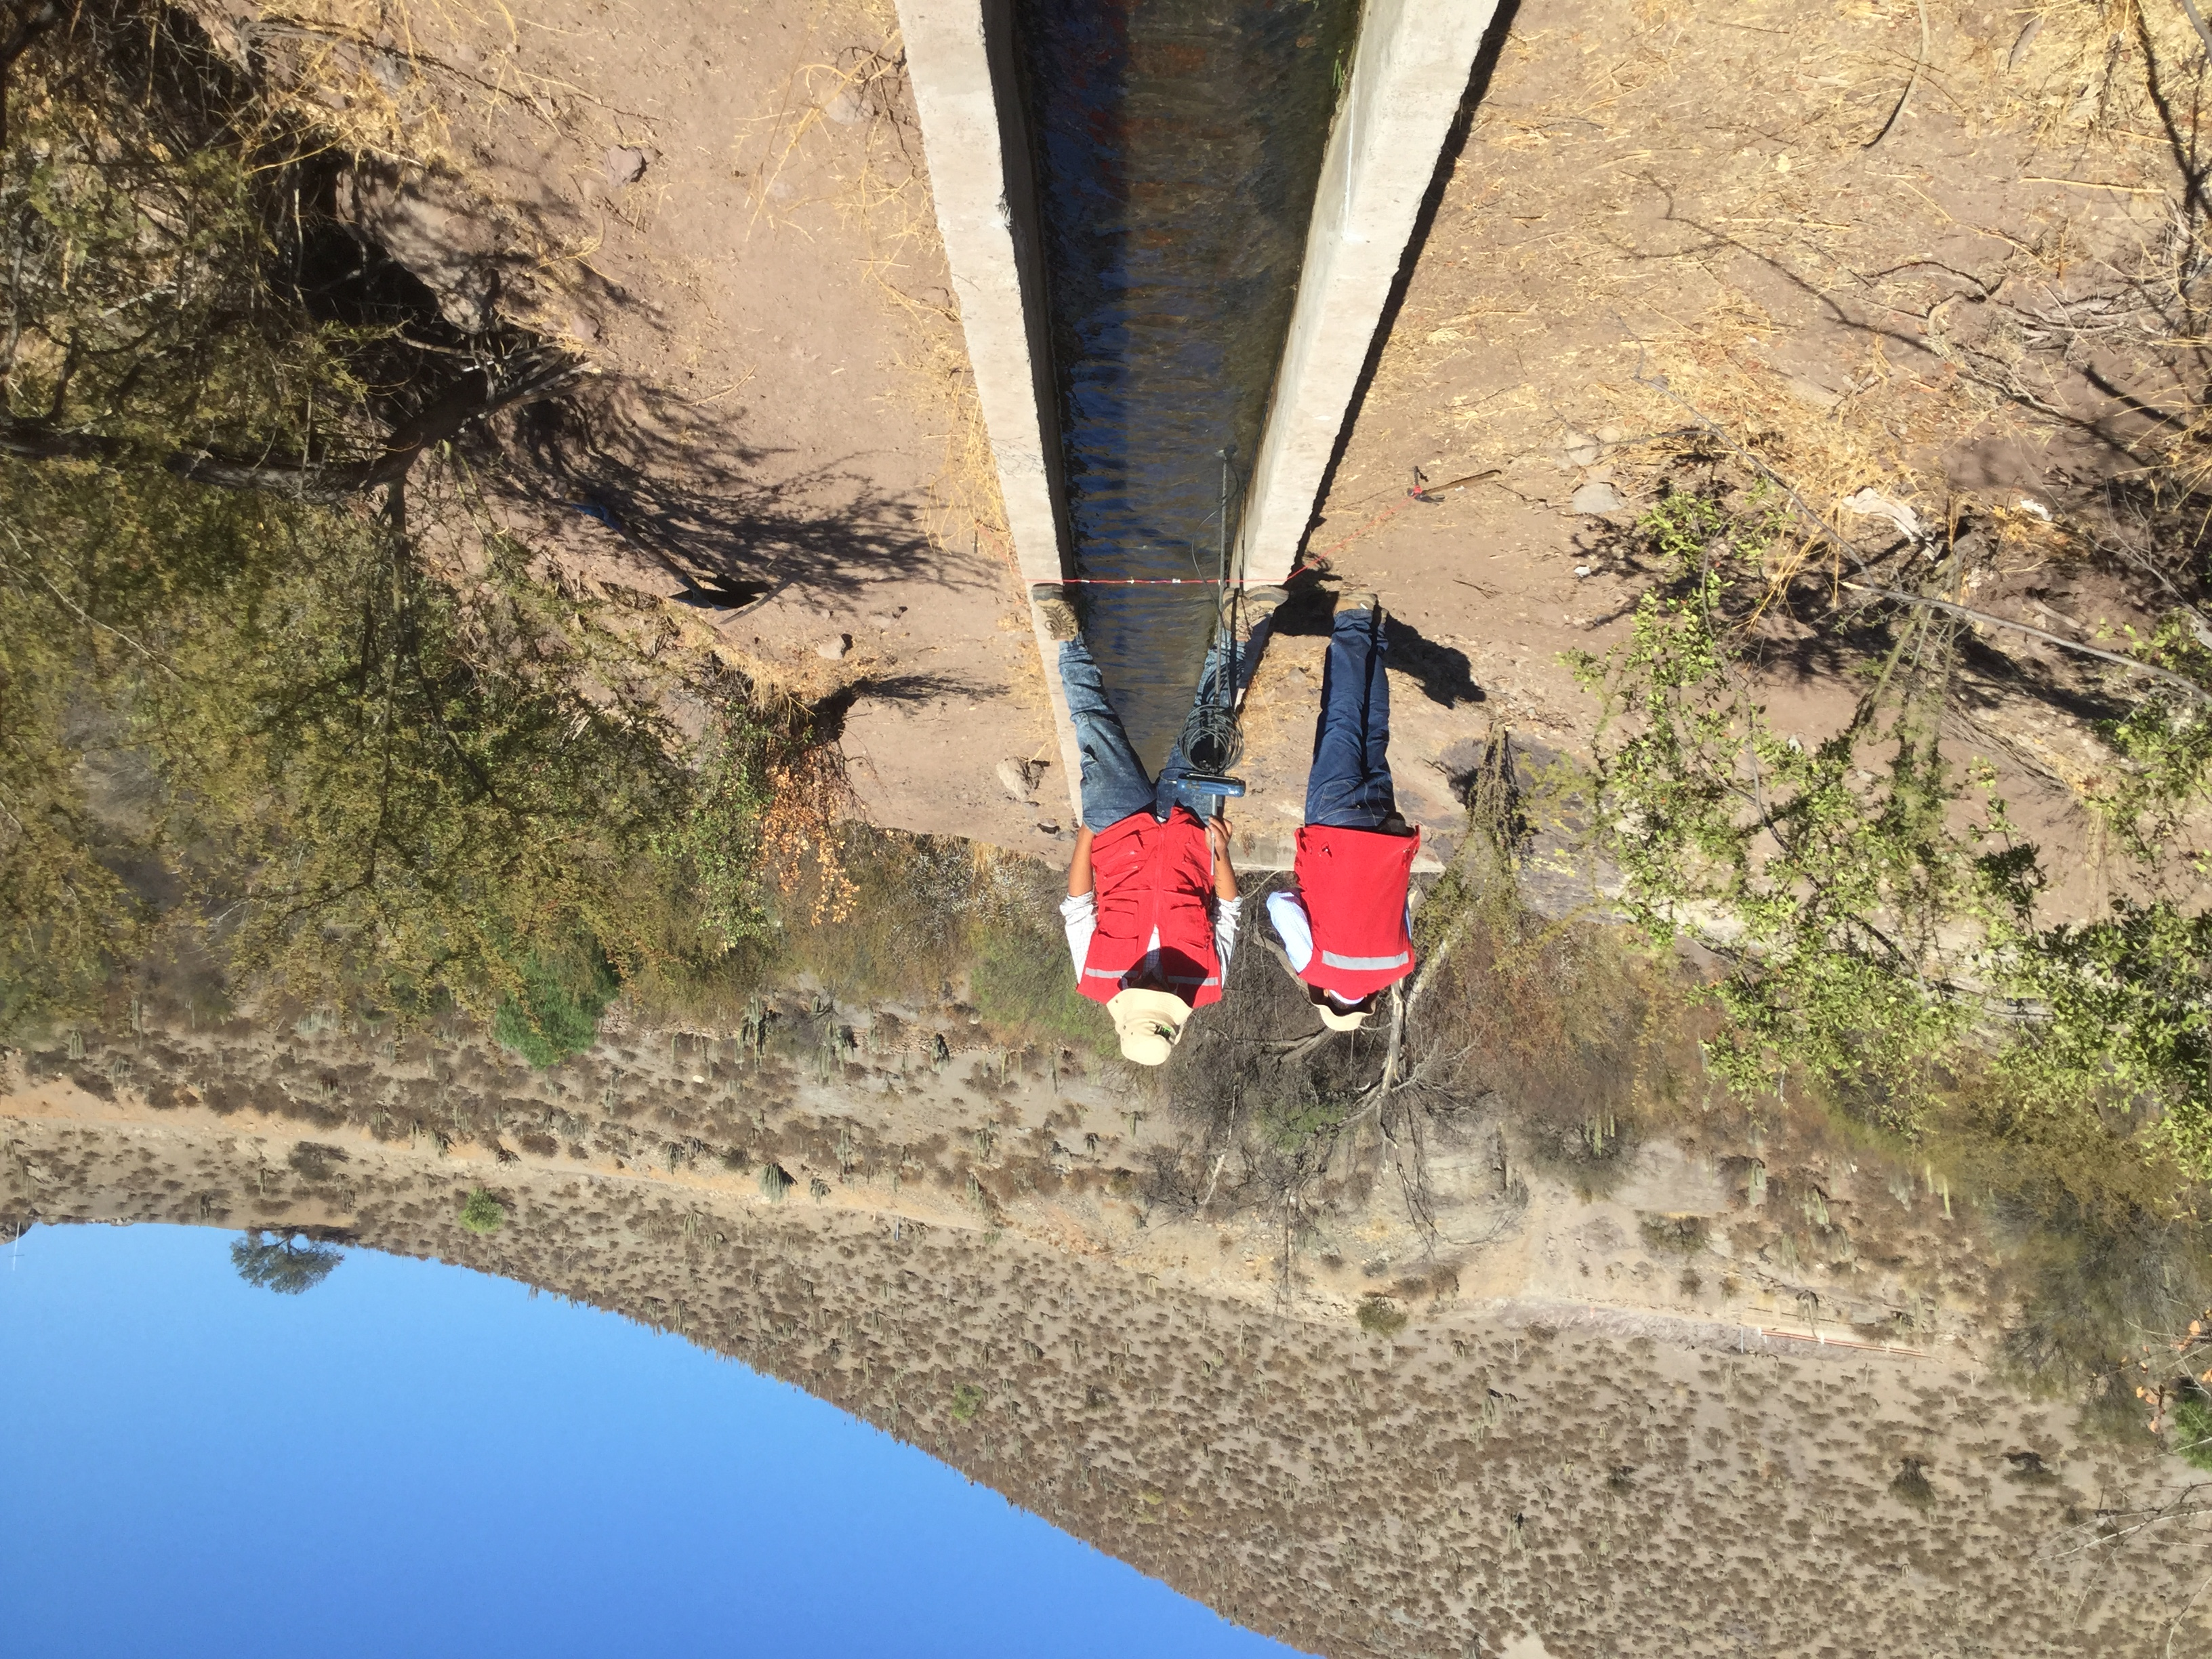
\includegraphics[angle= 180, width=\textwidth]{Foto/h3.jpg}
\end{subfigure}
\hfill
\begin{subfigure}{.45\textwidth}
\hfill
  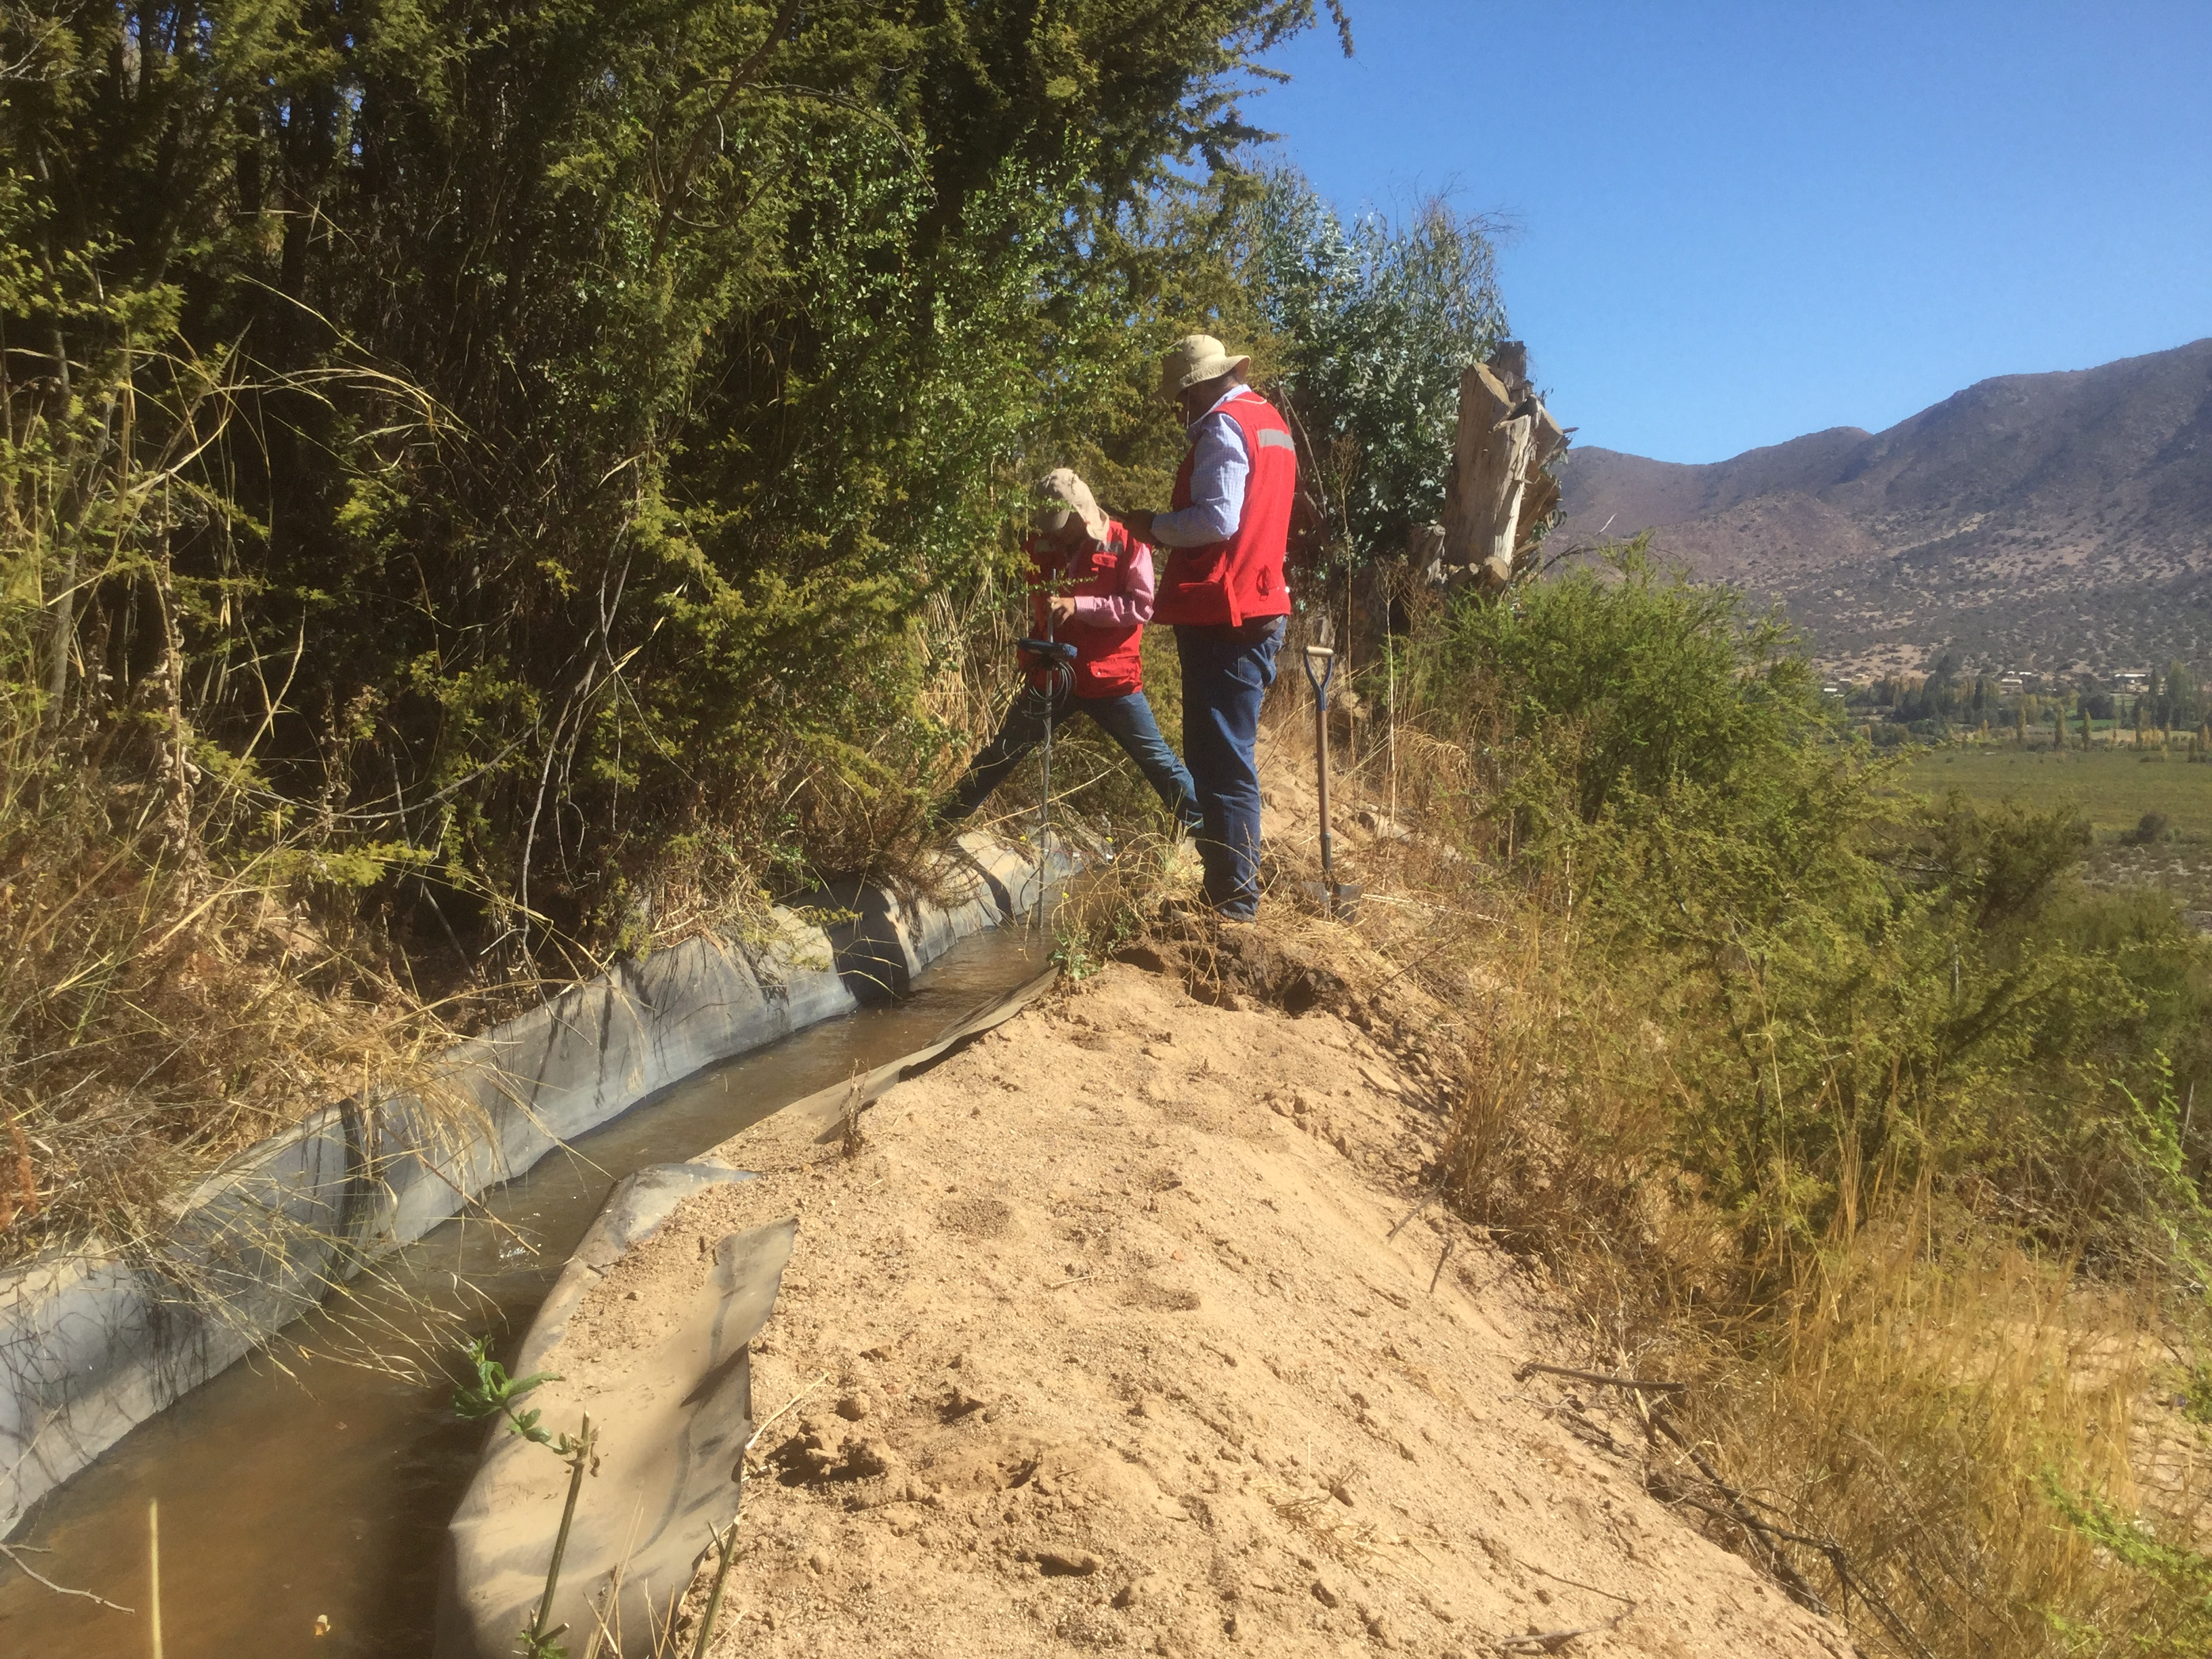
\includegraphics[width=\textwidth]{Foto/h4.jpg} 
\end{subfigure}
\caption{Aforos de caudal Canal Huanque, río Chalinga.}
\end{figure}


\end{document}